% PEPS
\noindent We consider a \textit{diagonal square lattice}, obtained from a 45-degree rotation of the conventional square lattice. Formally, it is defined as an $L_x \times L_y$ square \textit{Bravais lattice} (rescaled by $\sqrt{2}$), plus a two-spin \textit{basis} indexed by $p$:
\begin{equation} \label{eq:diagonal_square_lattice_1}
\begin{array}{cc}
	\raisebox{-0.5\height}{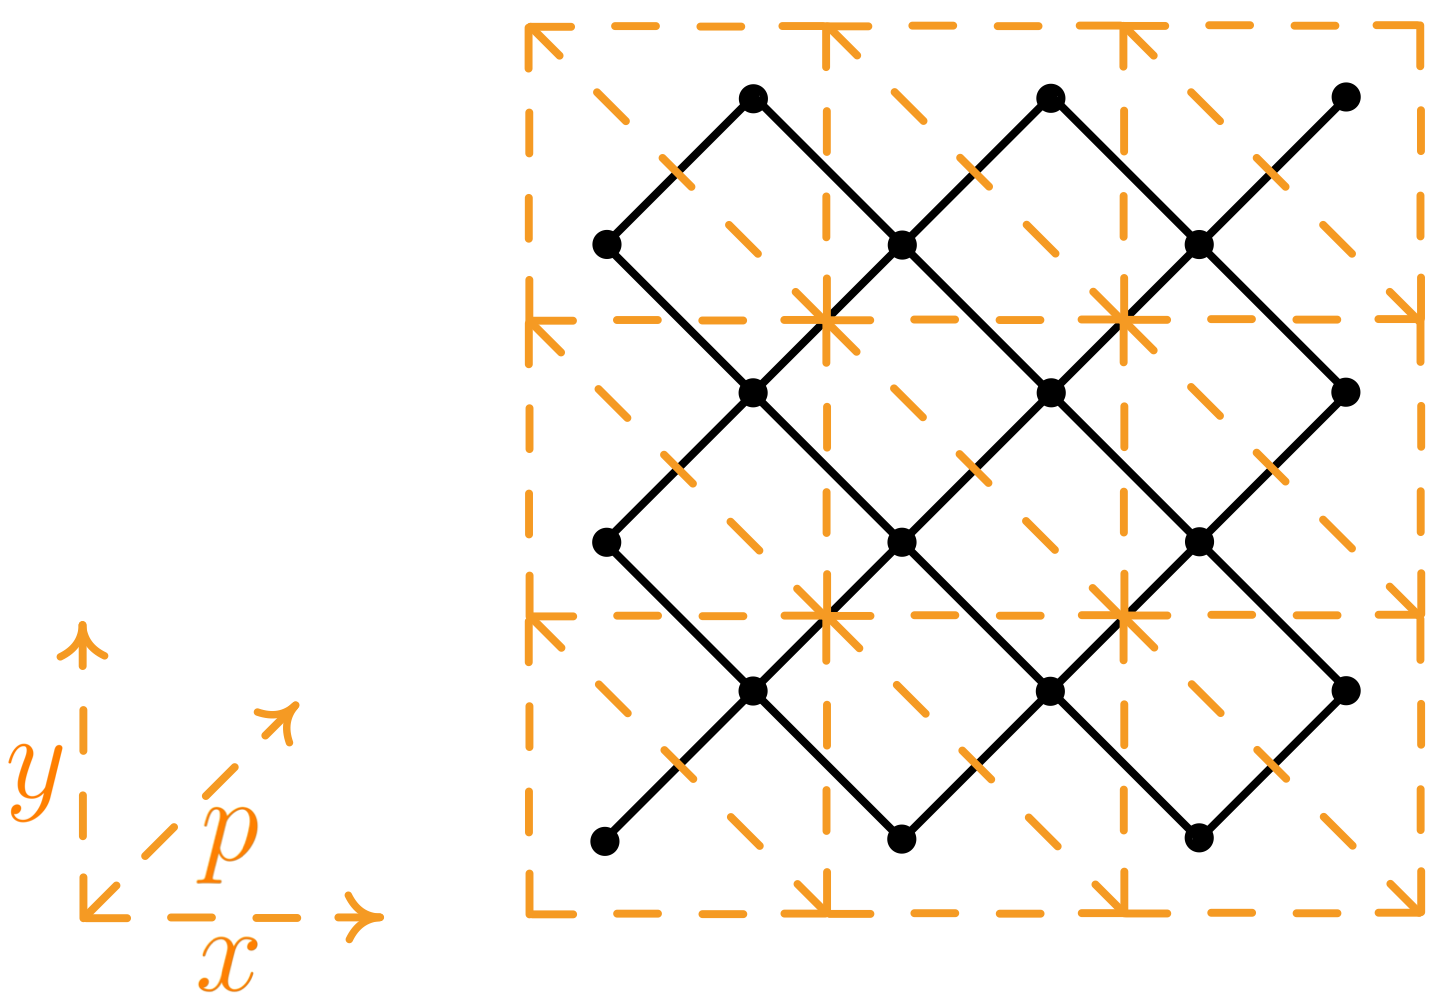
\includegraphics[height=4.5cm]{lattice1.png}} 
	&
	\begin{array}{l}
	\textcolor{orange}{x = 1, \ldots, L_x} \\
	\textcolor{orange}{y = 1, \ldots, L_y} \\
	\textcolor{orange}{p = 1, 2}
	\end{array}
\end{array}.
\end{equation}
Between all nearest neighbors of the $N = 2 L_x L_y$ sites, we distribute pairs of maximally entangled $D$-dimensional ancilla spins:
\begin{equation}
	\raisebox{-0.5\height}{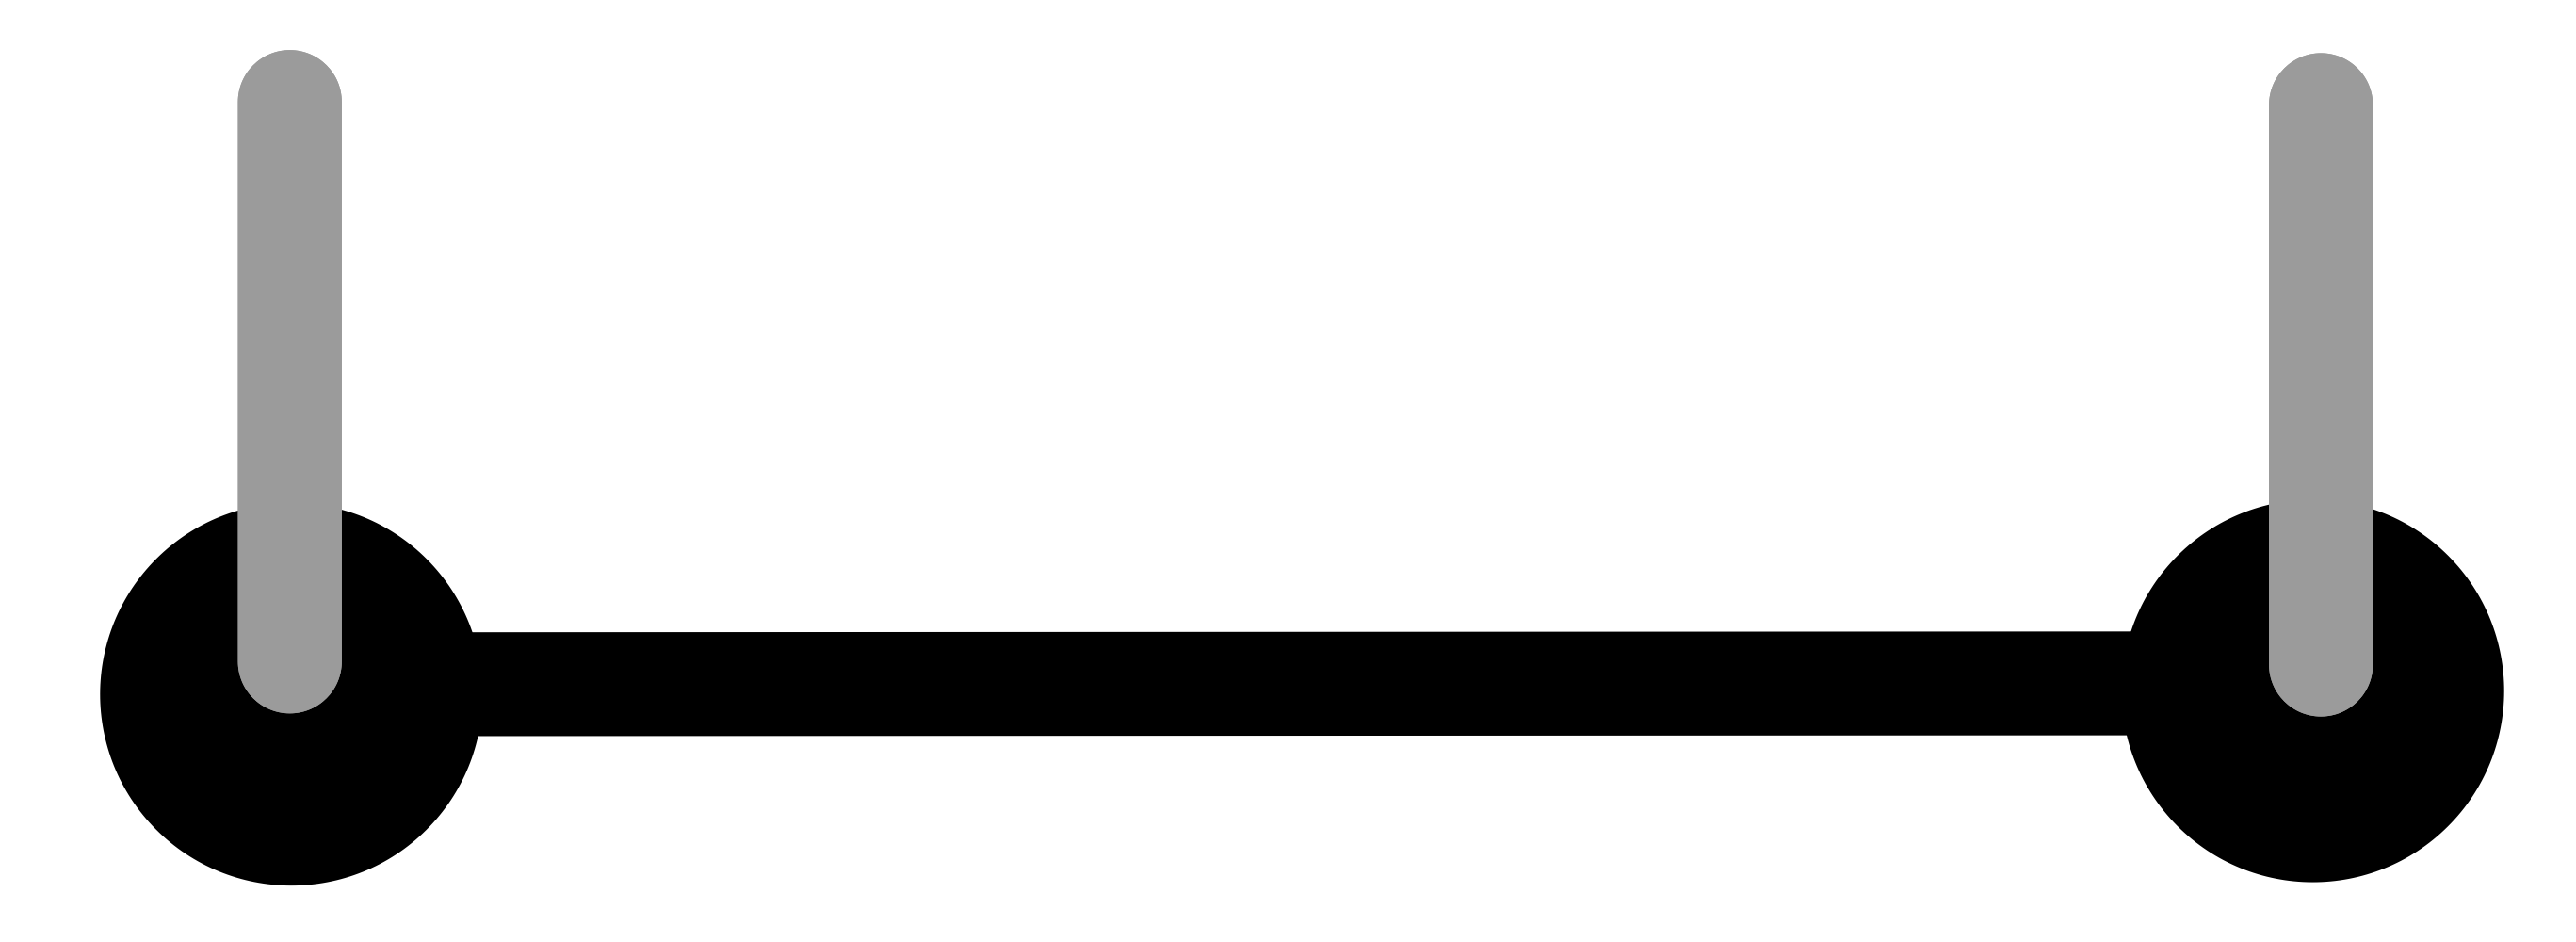
\includegraphics[height=0.5cm]{entangled_pair.png}} 
	\:=\: \sum_{\alpha = 1}^D \tket{\alpha \alpha} \in \mathbb{C}^{D} \otimes \mathbb{C}^{D} .
\end{equation}
On each site, we then apply the following projection onto a single $d$-dimensional physical spin:
\begin{equation}
	\raisebox{-0.5\height}{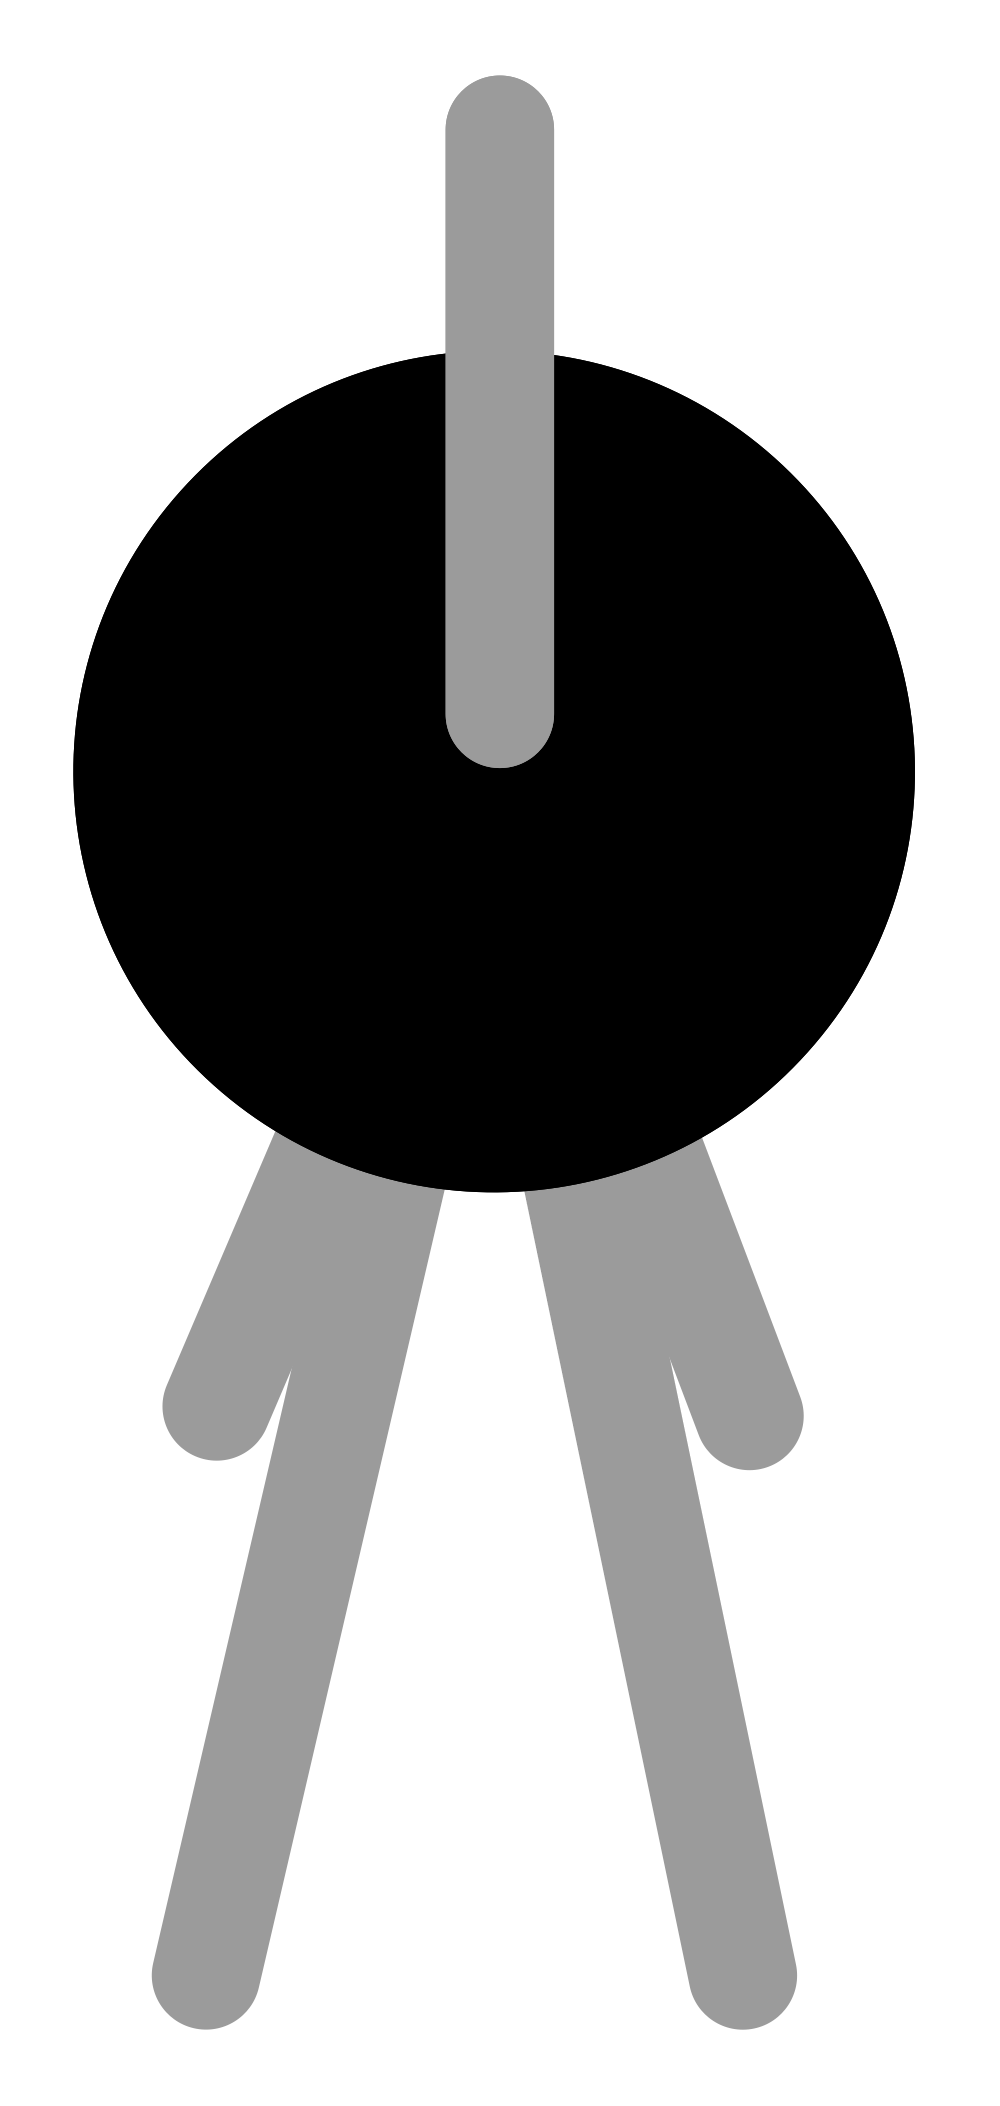
\includegraphics[height=1cm]{projection.png}} 
	\:=\: \sum_{s, \alpha, \beta, \gamma, \delta} A^{s}_{\alpha \beta \gamma \delta} \ket{s} \tbra{\alpha \beta \gamma \delta} \in \mathbb{C}^{d \times D^4} .
\end{equation}
This constructs a \textit{projected entangled pair state} (PEPS) \cite{verstraete2004renormalization} characterized by the five leg tensor $A \in \mathbb{C}^{d \times D \times D \times D \times D}$:
\begin{equation} \label{eq:peps}
	\ket{\psi(A)} 
	\:=\:
	\raisebox{-0.5\height}{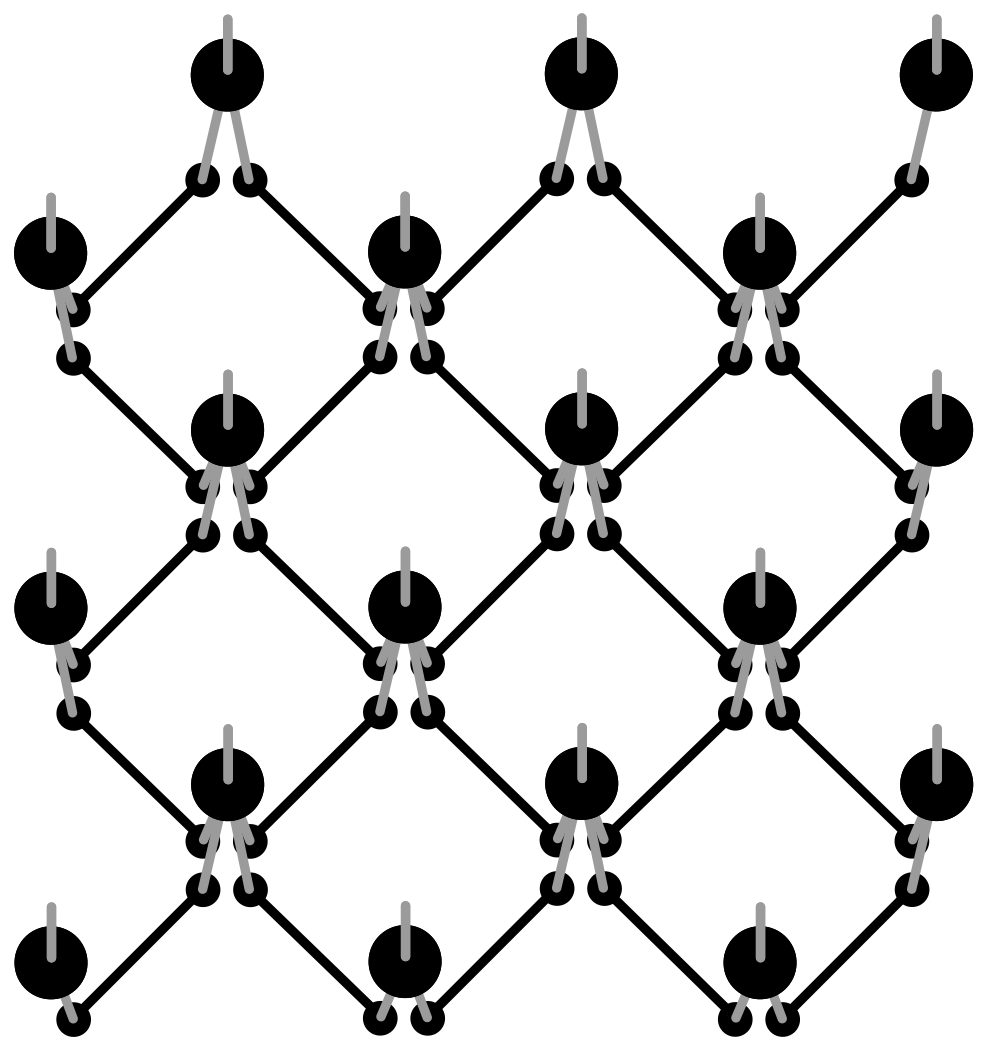
\includegraphics[height=4cm]{peps_construction.png}} 
	\:=\:
	\raisebox{-0.5\height}{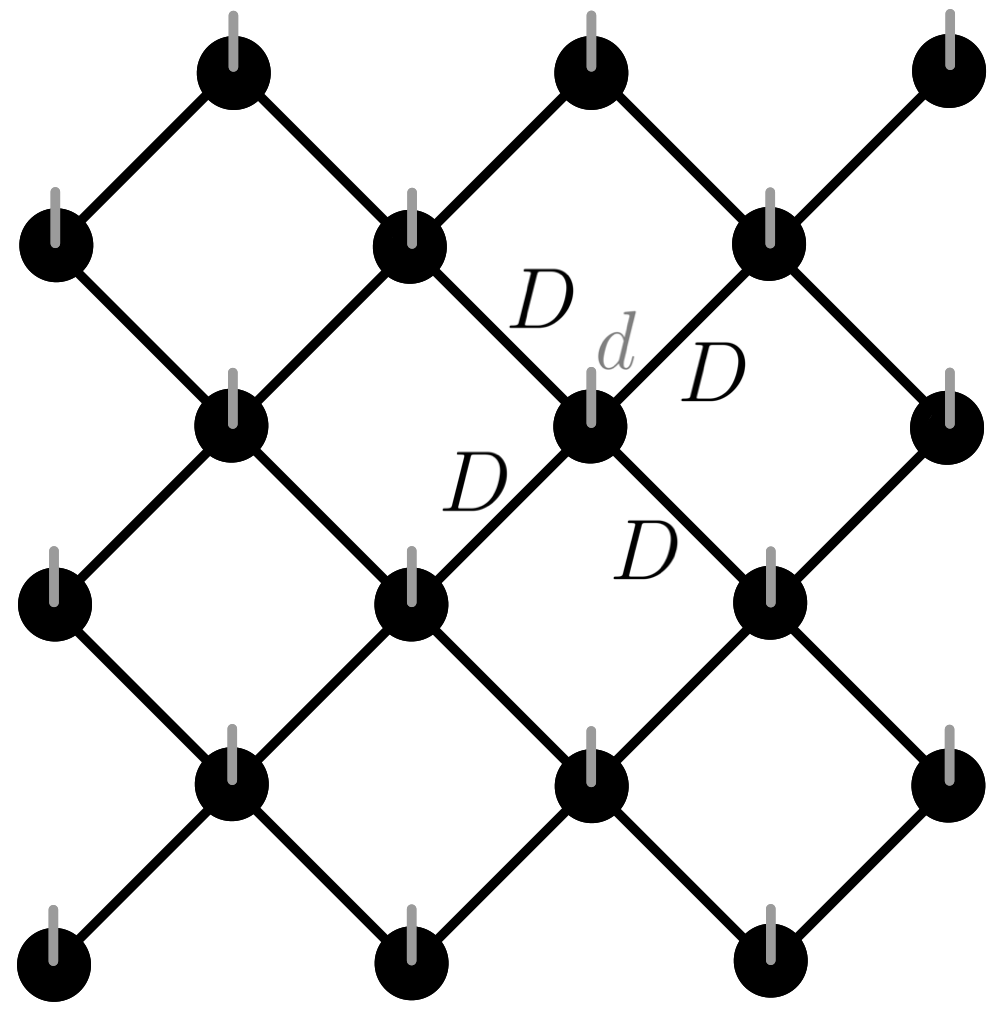
\includegraphics[height=4cm]{peps.png}} \hspace{0.2em} \in \mathbb{C}^{d^N}.
\end{equation}
Even though the ancilla spins are only locally entangled, the resulting correlations in the physical PEPS can be long-ranged. This is a consequence of \textit{entanglement swapping}, that is implemented through the sequence of projections applied to the entangled pairs. Nevertheless, the local connectivity of tensors with finite bond dimension enforces the \textit{area law}. Specifically, the total amount of entanglement between a subregion $\mathcal{R}$ of spins and its complement is upper bounded by the size of the boundary $\vert \partial \mathcal{R} \vert$:
\begin{equation} \label{eq:area_law_peps}
\begin{array}{cc}
	\raisebox{-0.5\height}{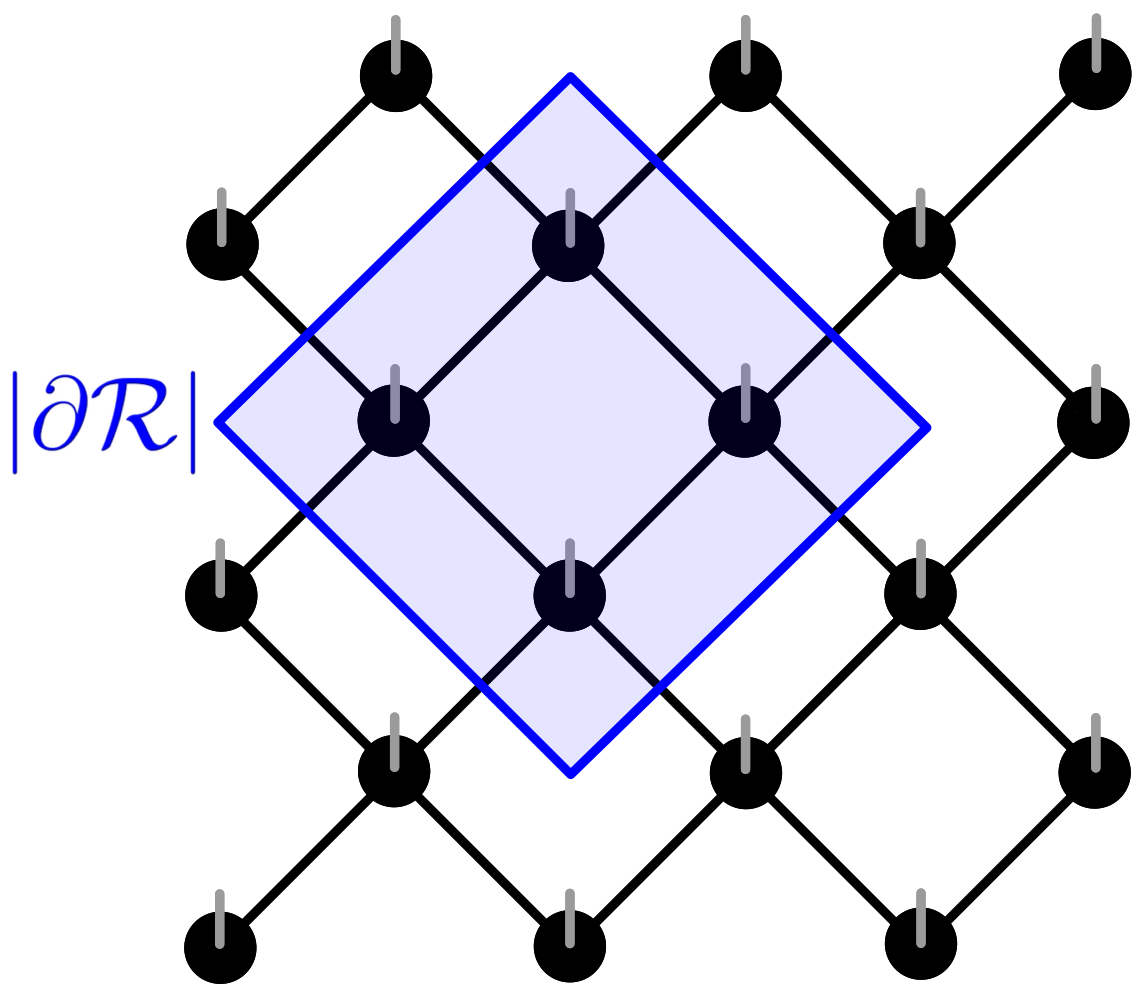
\includegraphics[height=4cm]{peps_area.png}} 
	& 
	S(\psi_A) = -\tr[\rho_{\mathcal{R}} \log \rho_{\mathcal{R}}] \leq \vert \partial \mathcal{R} \vert \log D.
\end{array}
\end{equation}
Although not rigorously proven in two dimensions, it is conjectured that ground states of local, gapped Hamiltonians fulfill a generalization of \eqref{eq:area_law} with the form of \eqref{eq:area_law_peps}, i.e. that PEPS can faithfully represent 2D ground states \cite{cirac2021matrix}. \\[1em]
\noindent Note that we impose open boundary conditions, which reduce the number of nearest neighbors at the edges and require the affected tensors to be adjusted in dimensions accordingly---for example, by taking slices of the bulk tensor $A$. As we will specify in the following section, we allow the tensors to be site-dependent anyway. 

% CANONICAL FORM AND YANG-BAXTER MOVE
\section{Imposed canonical form and Yang-Baxter move} \label{sec:canonical_form_yb}
By cutting a single leg, one cannot disconnect the tensor network \eqref{eq:peps} into two disjoint parts free from any loops. This makes it impossible to bring a general PEPS into canonical form as we know it for MPS. Even if one removes inter-loops by cutting multiple legs, the remaining intra-loops still prevent the subsystems from being orthonormalized. In particular, one cannot isolate an orthogonality center with ingoing legs only within the PEPS gauge freedom. We circumvent this by imposing an isometric form that restricts the variational class to a strict PEPS subset: the \textit{isometric projected entangled pair states} (isoPEPS). They were introduced by \cite{zaletel2020isometric} and computationally investigated in more technical detail by \cite{lin2022efficient}, both for the conventional square lattice. In our work, we adopt the rotated version developed in the master's thesis \cite{sappler2024diagonal, sappler2025diagonal}. \\[0.5em]

% imposed canonical form
\noindent \underline{Imposed canonical form} \\[0.5em]
\noindent Being more convenient for indexing the isometric tensors, we introduce columns $n_x = 2(x-1) + p$ in our lattice \eqref{eq:diagonal_square_lattice_1}:
\begin{equation} \label{eq:diagonal_square_lattice_2}
\begin{array}{cc}
	\raisebox{-0.5\height}{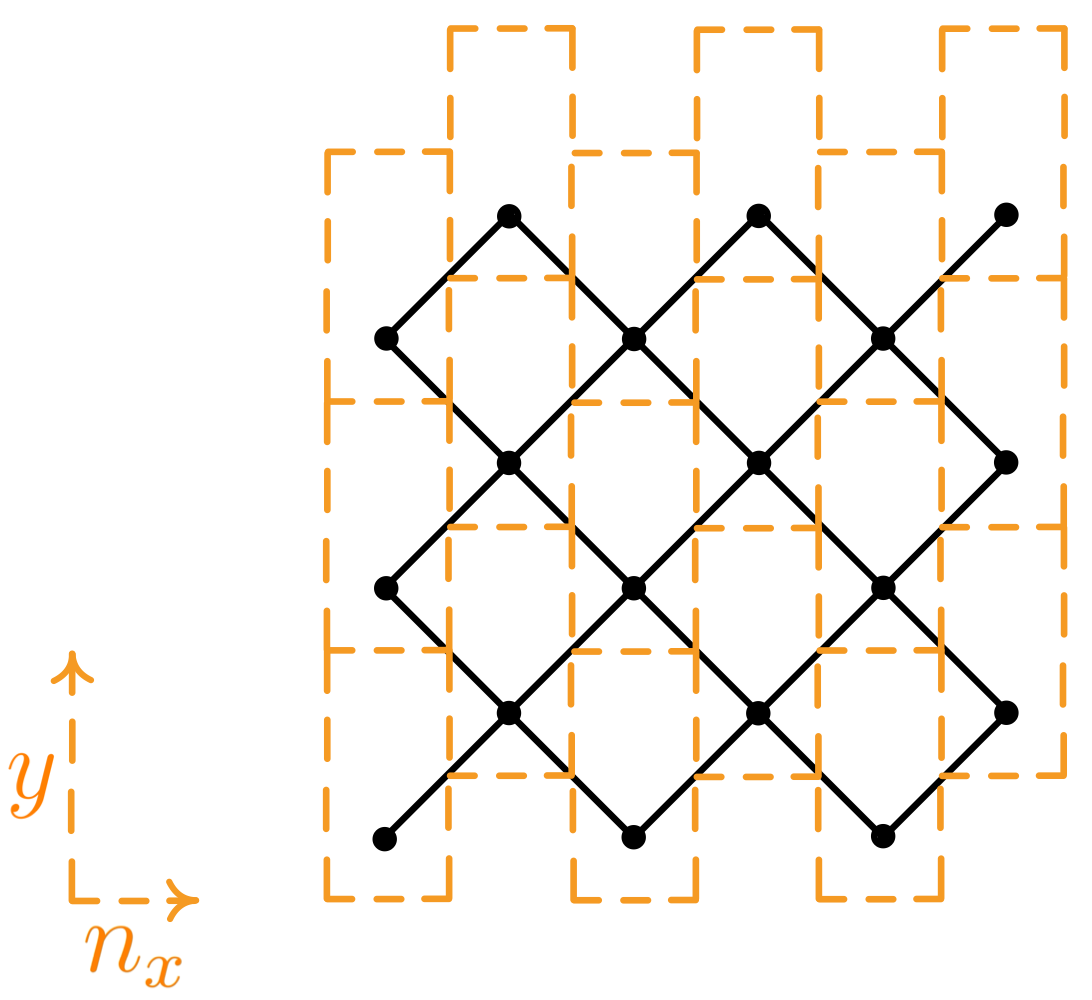
\includegraphics[height=5cm]{lattice2.png}} 
	&
	\begin{array}{l}
	\textcolor{orange}{n_x = 1, \ldots, 2L_x} \\
	\textcolor{orange}{y = 1, \ldots, L_y} \\
	\end{array}
\end{array}.
\end{equation}
We choose one \textit{orthogonality column} $n_x^c \in \{0, 1, \ldots, 2 L_x\}$ and demand the $A$-tensors for $n_x \leq n_x^c$ to be left isometric and those for $n_x > n_x^c$ to be right isometric, in the following way:
\begin{align} 
	A_L^{[n_x \leq n_x^c, y]} \label{eq:AL}
	&\:=\:
	\raisebox{-0.5\height}{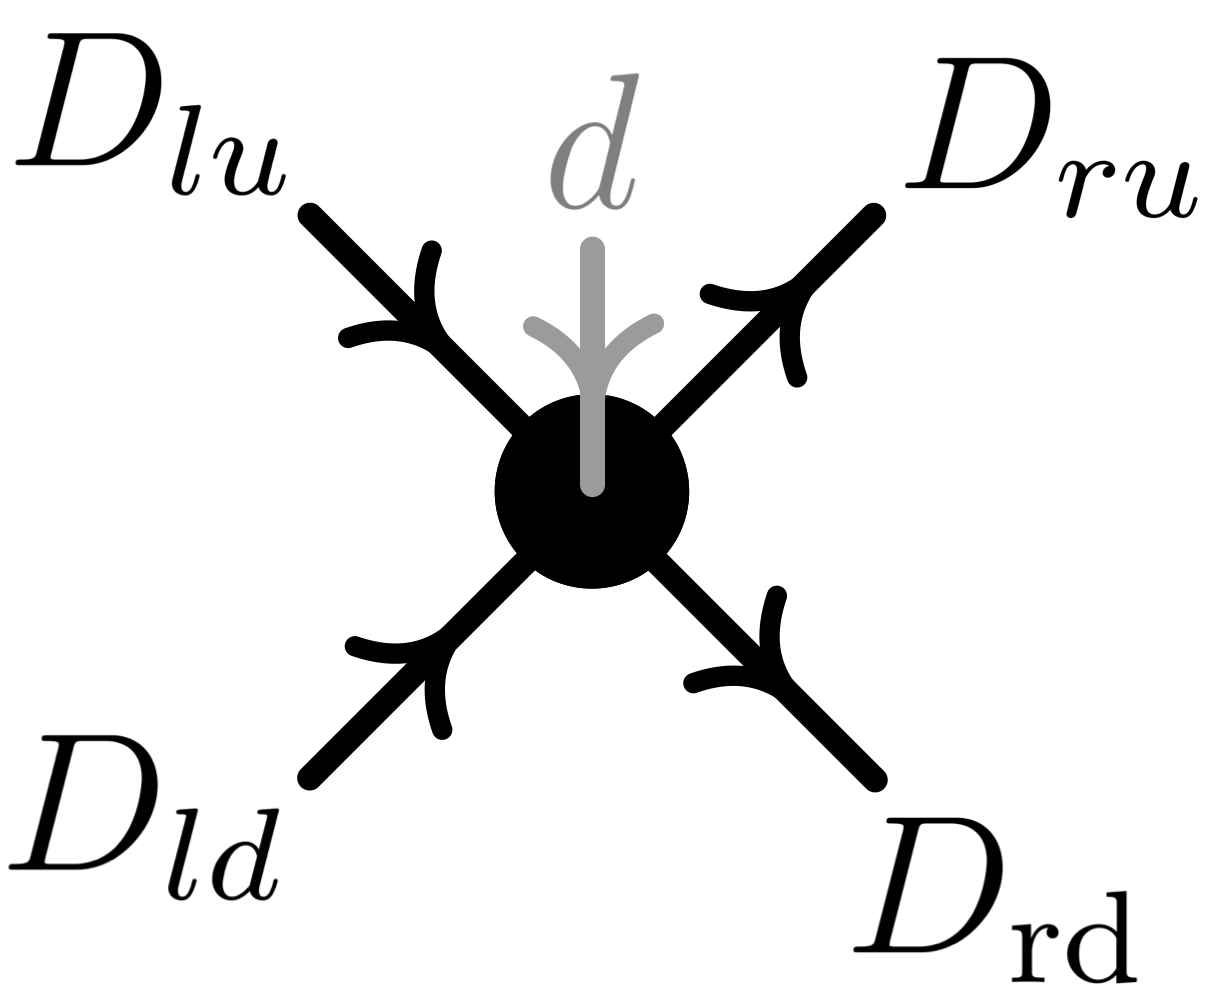
\includegraphics[height=1.7cm]{AL.png}}
	\:\text{ with }\:
	\raisebox{-0.5\height}{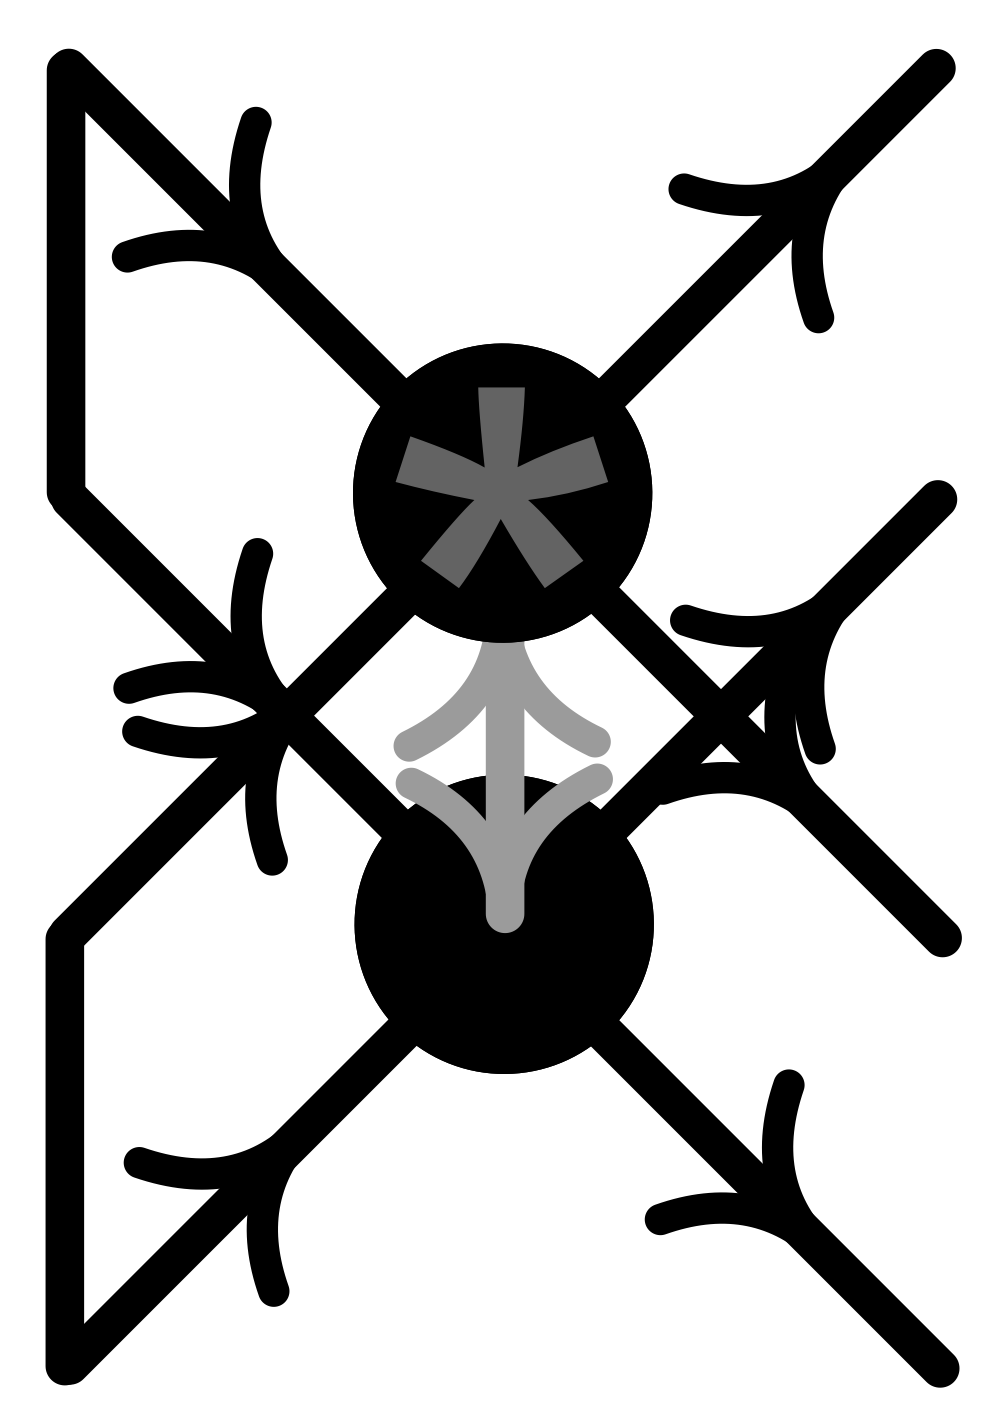
\includegraphics[height=1.4cm]{AL_contracted.png}}
	\:=\:
	\raisebox{-0.5\height}{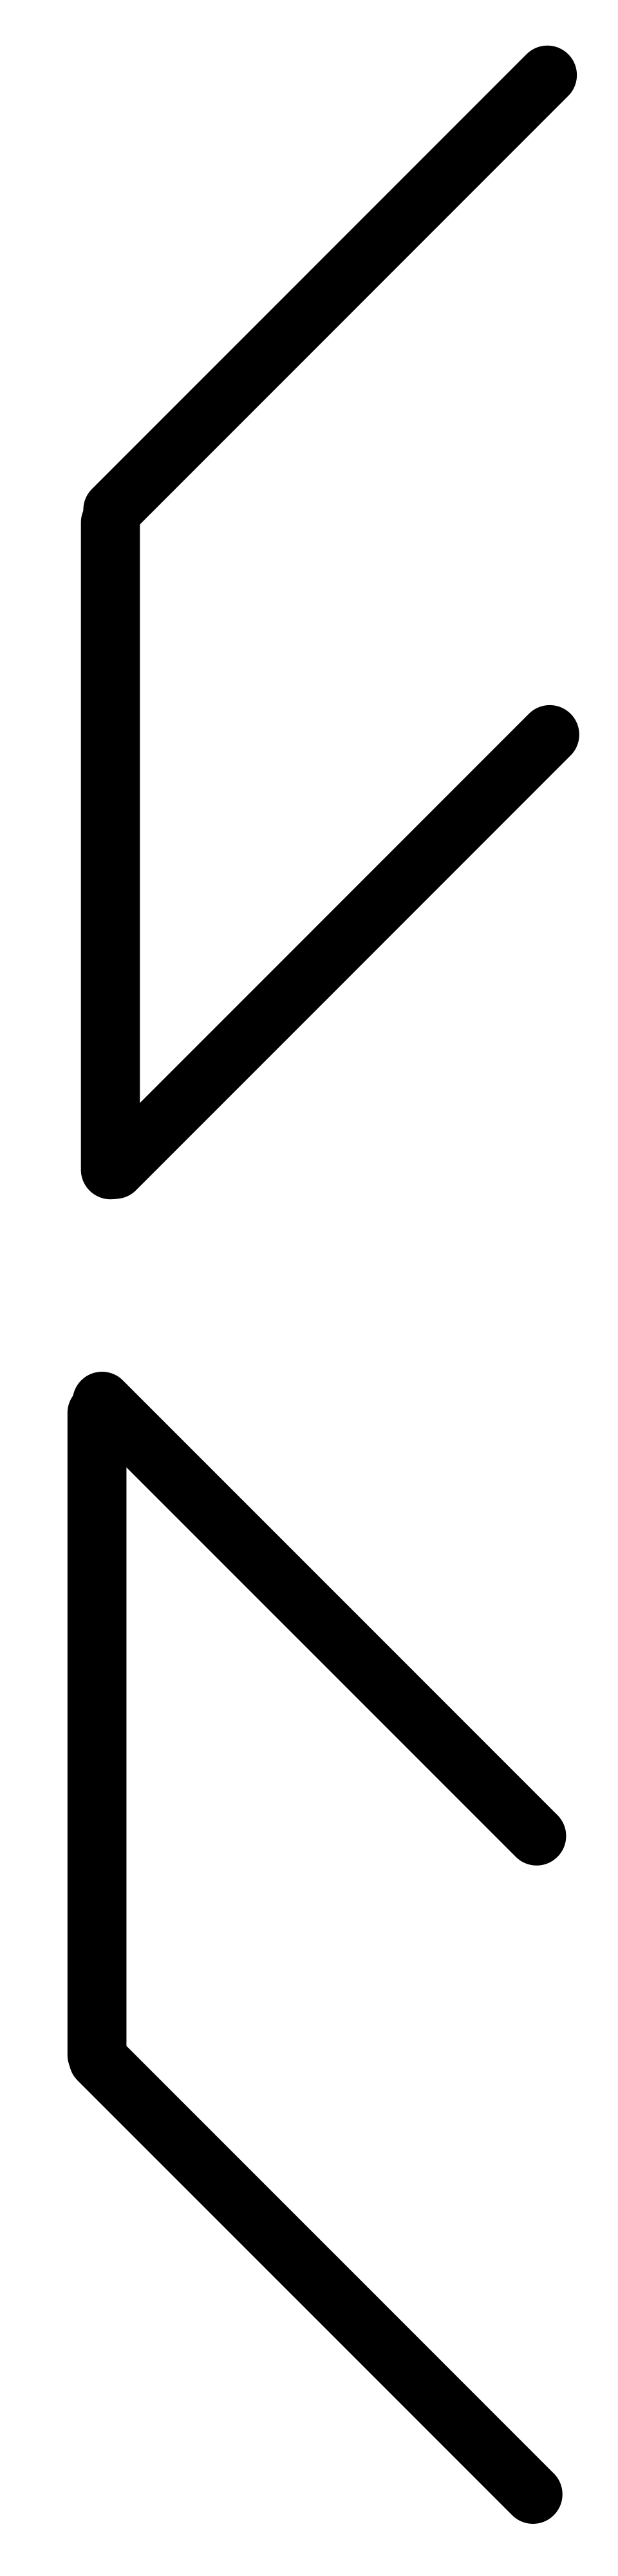
\includegraphics[height=1.8cm]{AL_id.png}} \hspace{0.2em},
\\
	A_R^{[n_x > n_x^c, y]} \label{eq:AR}
	&\:=\:
	\raisebox{-0.5\height}{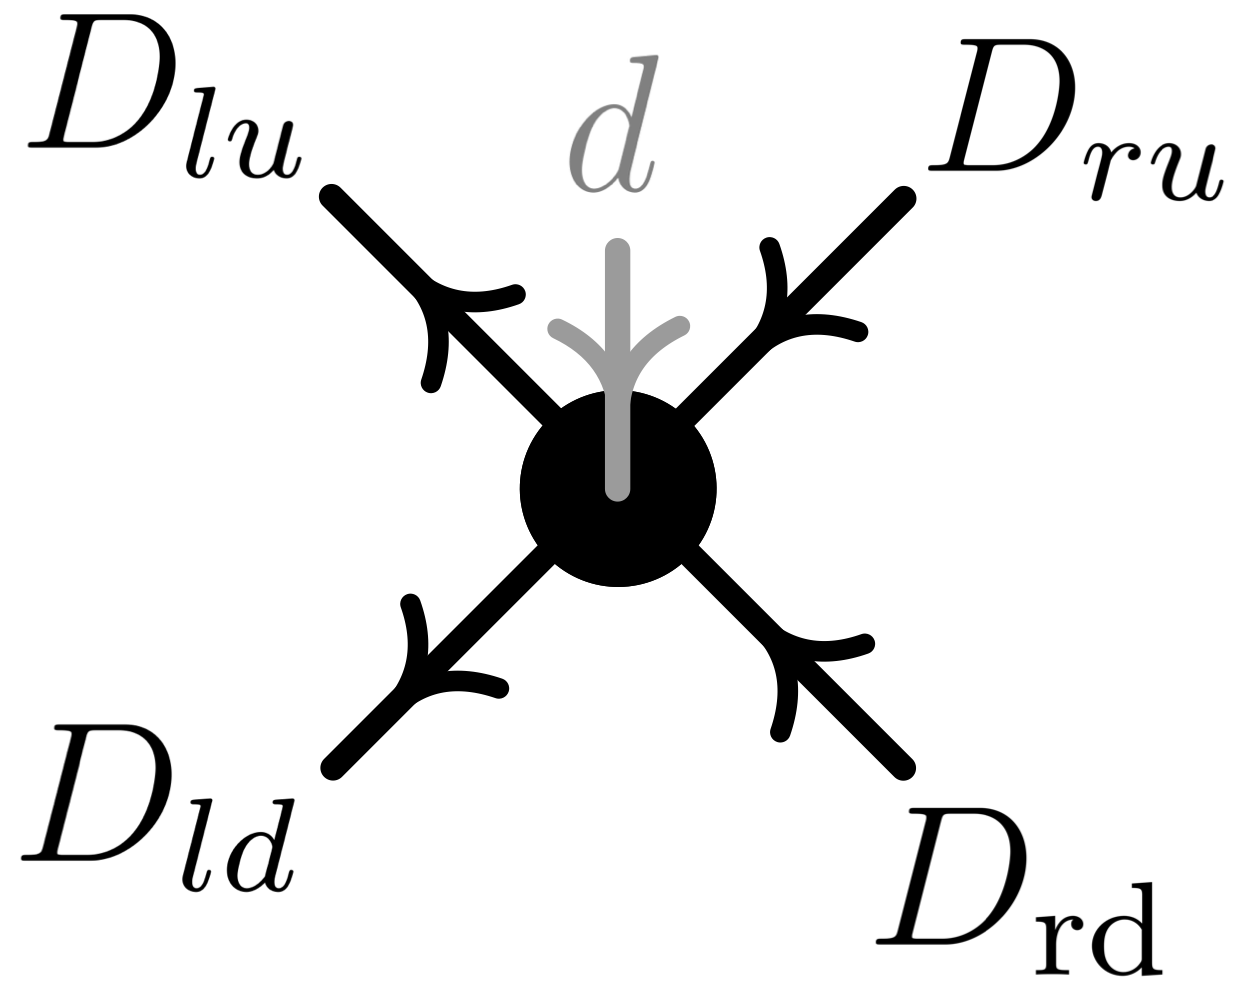
\includegraphics[height=1.7cm]{AR.png}}
	\:\text{ with }\:
	\raisebox{-0.5\height}{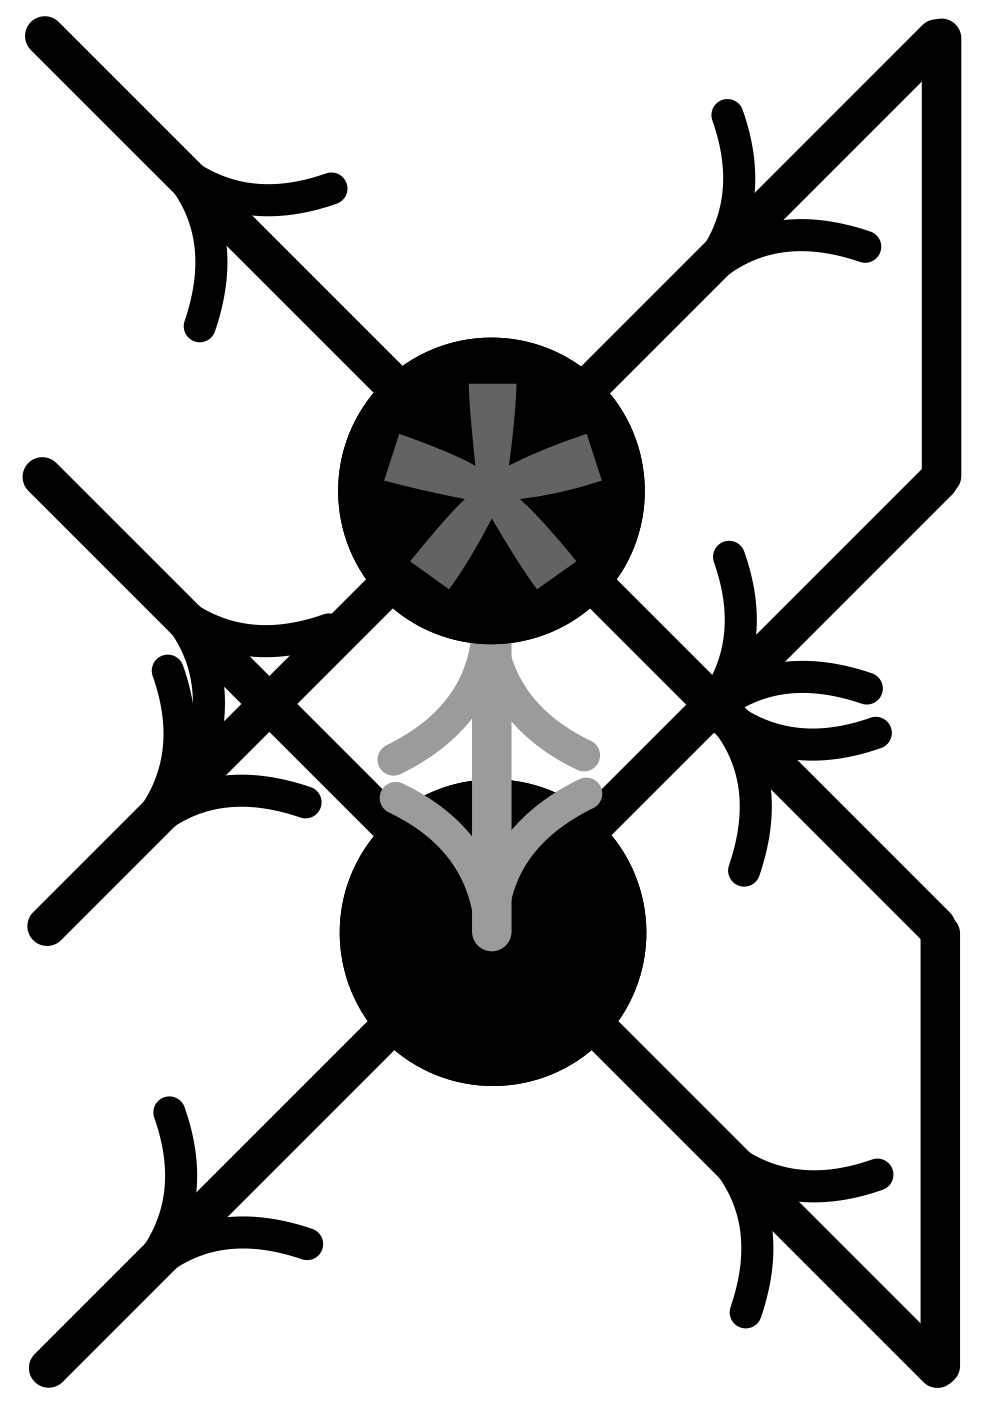
\includegraphics[height=1.4cm]{AR_contracted.png}}
	\:=\:
	\raisebox{-0.5\height}{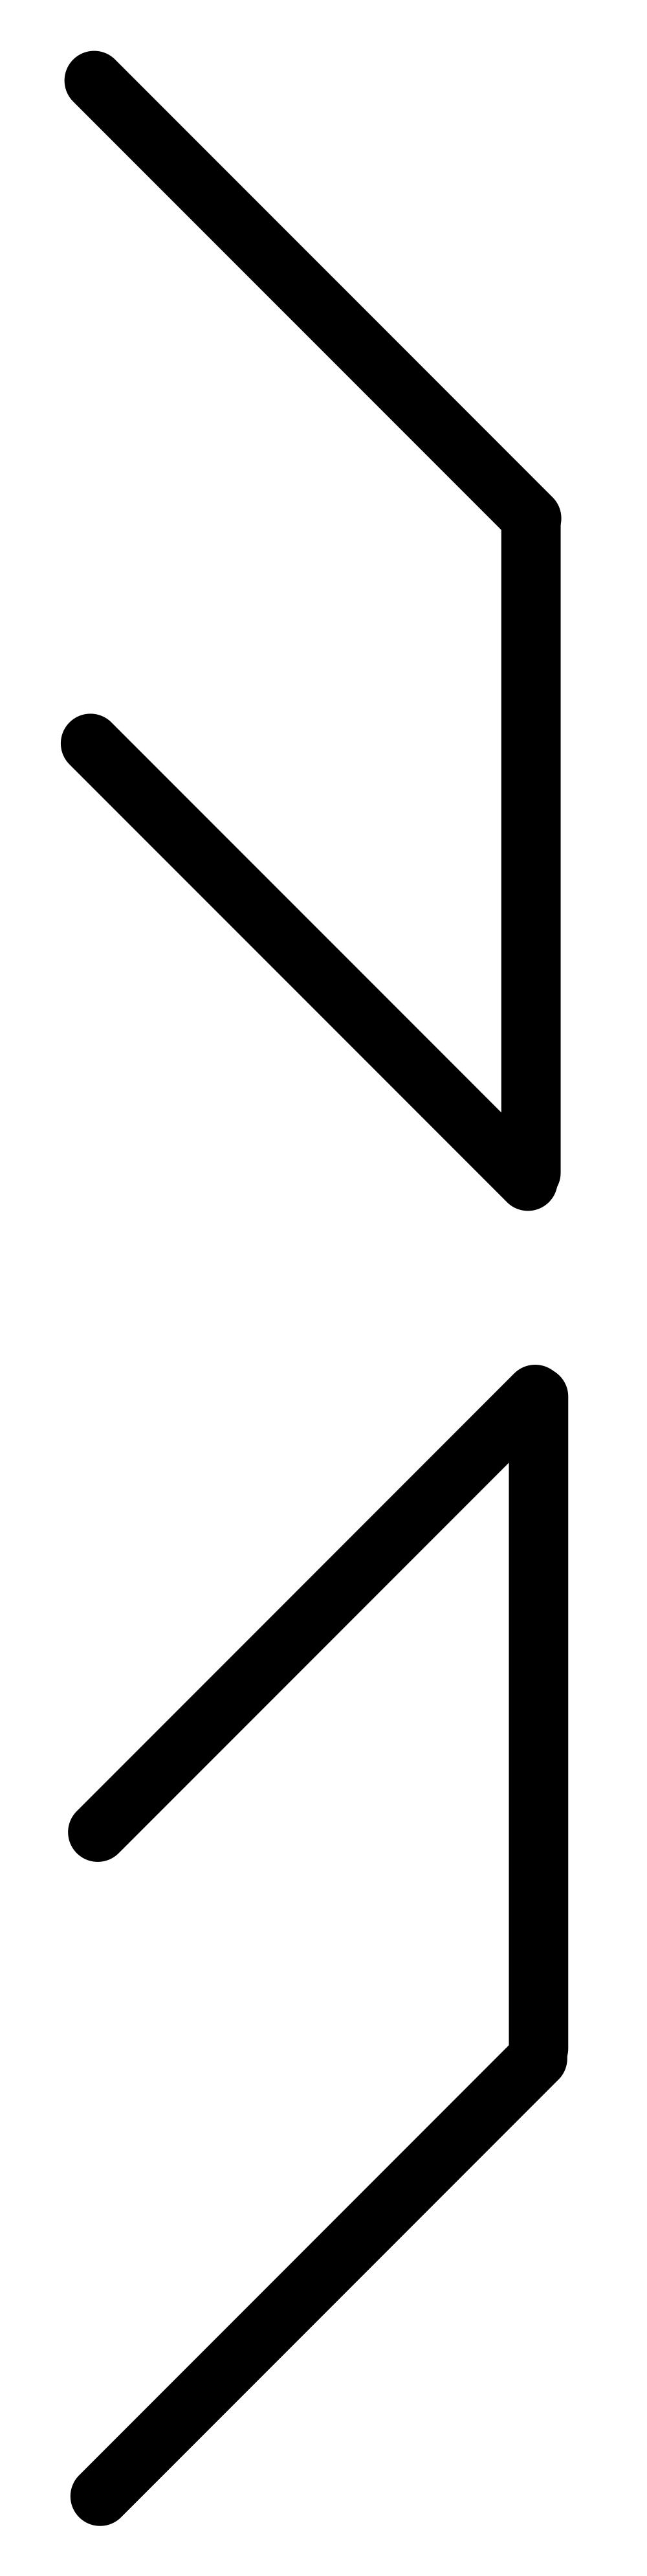
\includegraphics[height=1.8cm]{AR_id.png}} \hspace{0.2em}.
\end{align}
Between $A_L^{[n_x^c]}$ and $A_R^{[n_x^c + 1]}$ we then insert a column $C^{[n_x^c]}$ of rank-4 auxiliary tensors $C^{[n_x^c, n_y]}$ for $n_y = 1, \ldots, 2L_y-1$. We complete the ingoing arrows from left and right with vertical arrows pointing towards a single \textit{orthogonality center} $(n_x^c, n_y^c)$. In other words, there is a normalized center tensor $C_C^{[n_x^c, n_y^c]}$, connected to \textit{up isometries} $C_U^{[n_x^c, n_y > n_y^c]}$ from above and to \textit{down isometries} $C_D^{[n_x^c, n_y < n_y^c]}$ from below:
\begin{align} 
	C_U^{[n_x^c, n_y > n_y^c]} \label{eq:CU}
	&\:=\:
	\raisebox{-0.5\height}{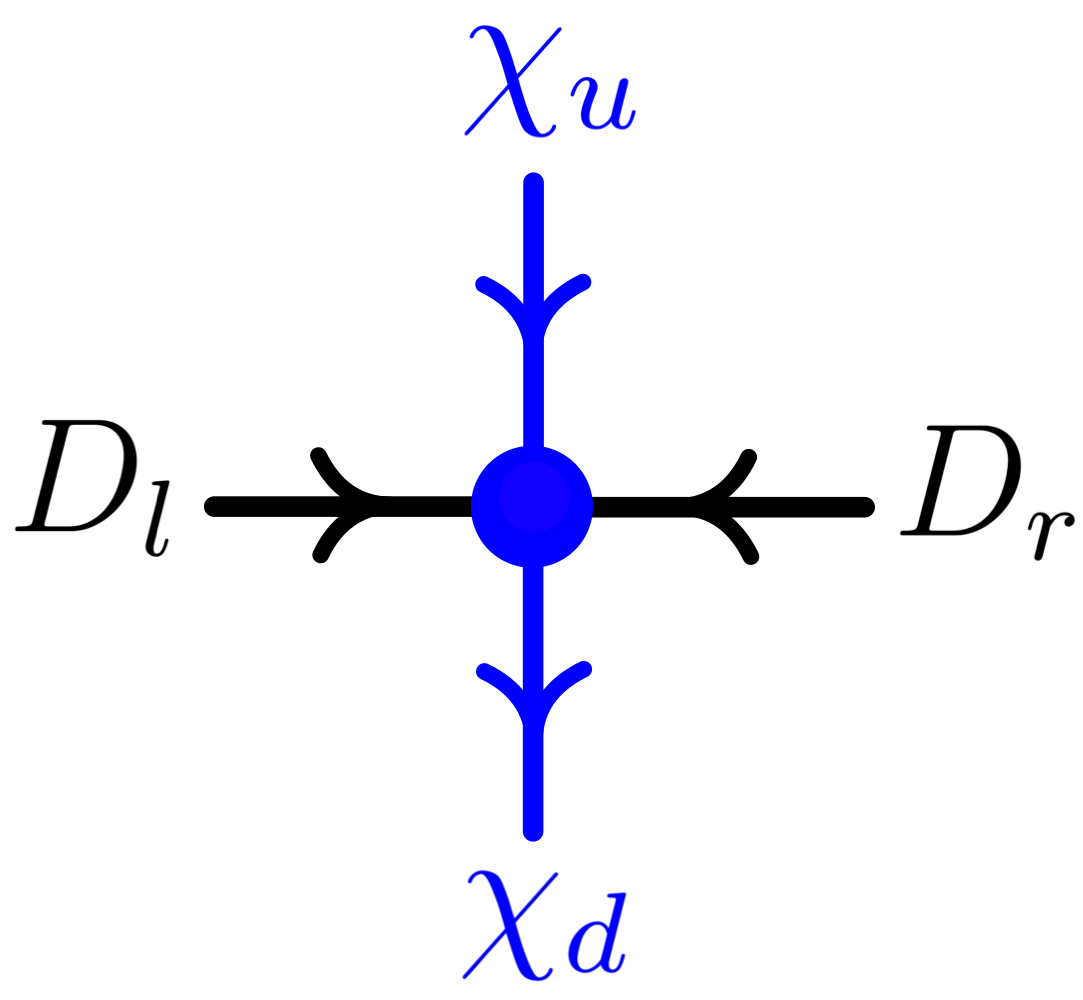
\includegraphics[height=1.9cm]{CU.png}}
	\:\text{ with }\:
	\raisebox{-0.5\height}{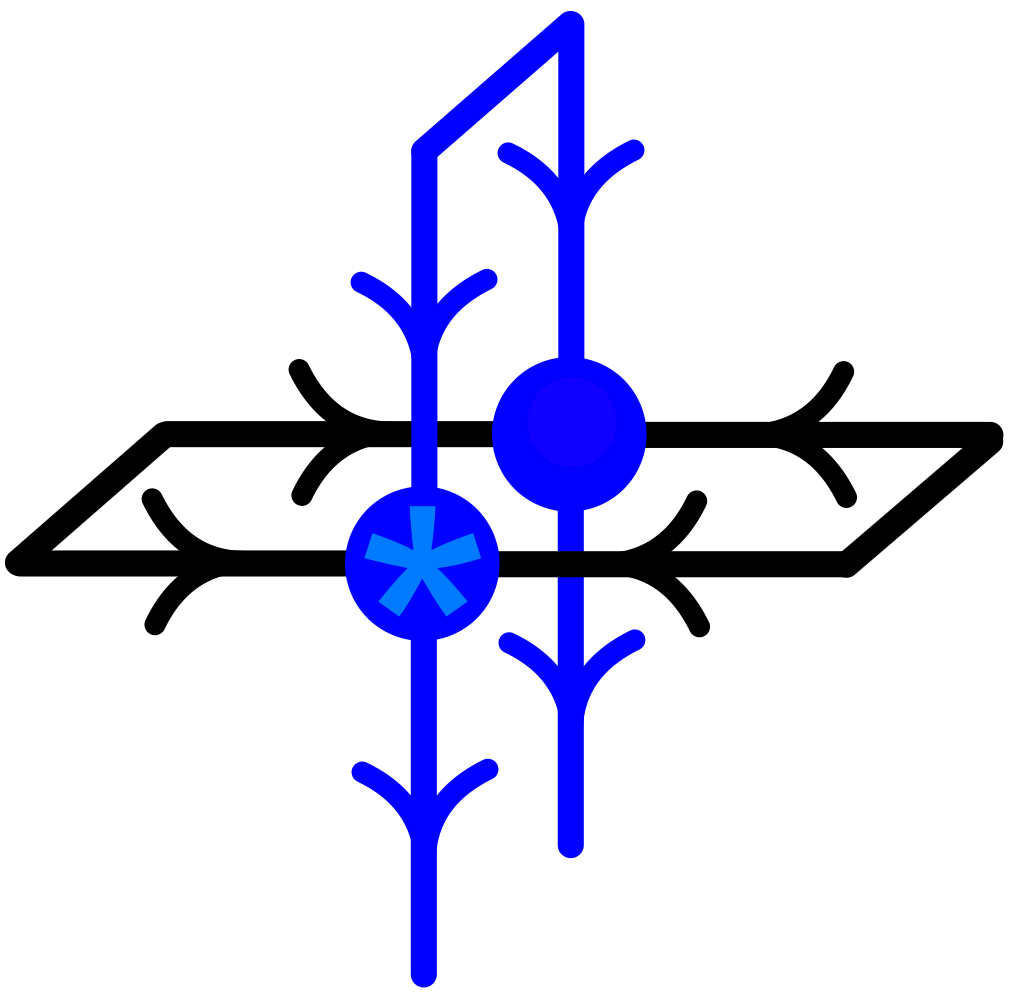
\includegraphics[height=1.5cm]{CU_contracted.png}}
	\:=\:
	\raisebox{-0.5\height}{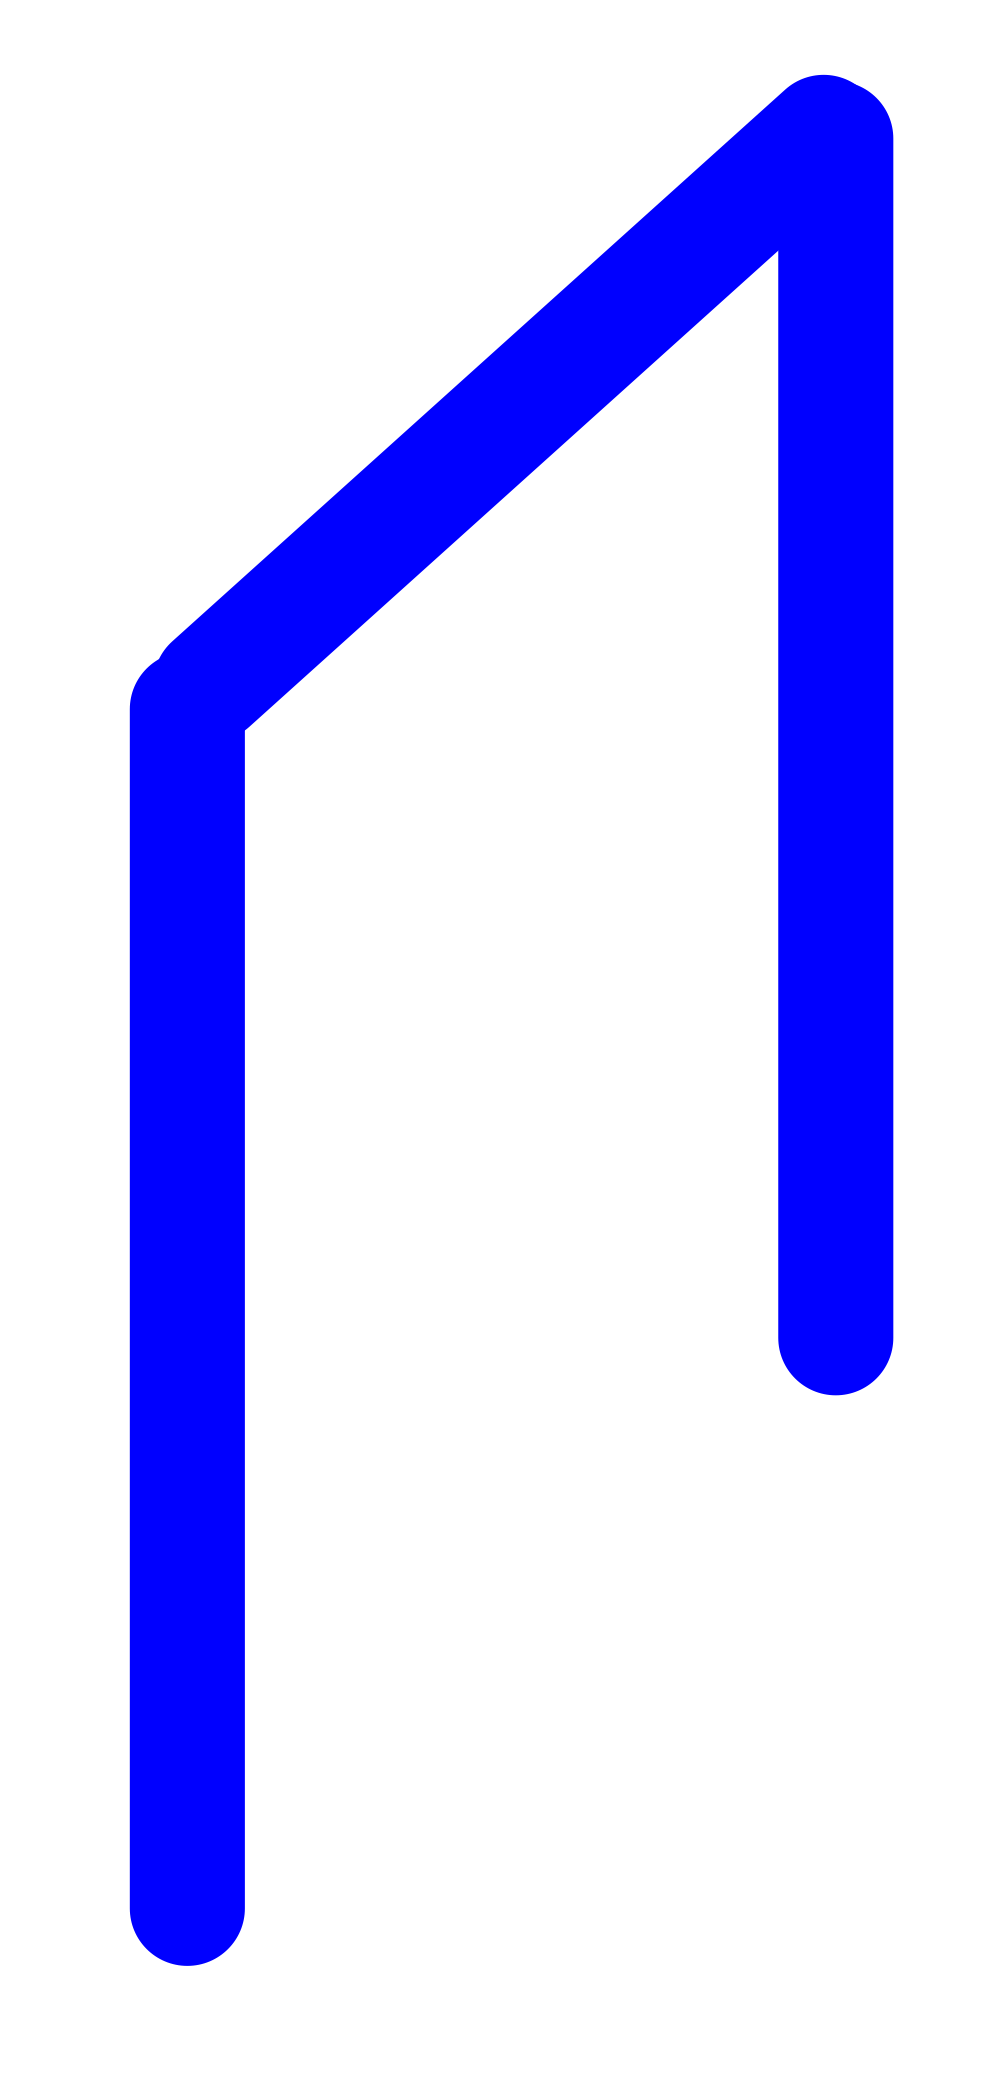
\includegraphics[height=0.9cm]{CU_id.png}} 
	\hspace{0.2em},
\\
	C_C^{[n_x^c, n_y^c]} \label{eq:CC}
	&\:=\:
	\raisebox{-0.5\height}{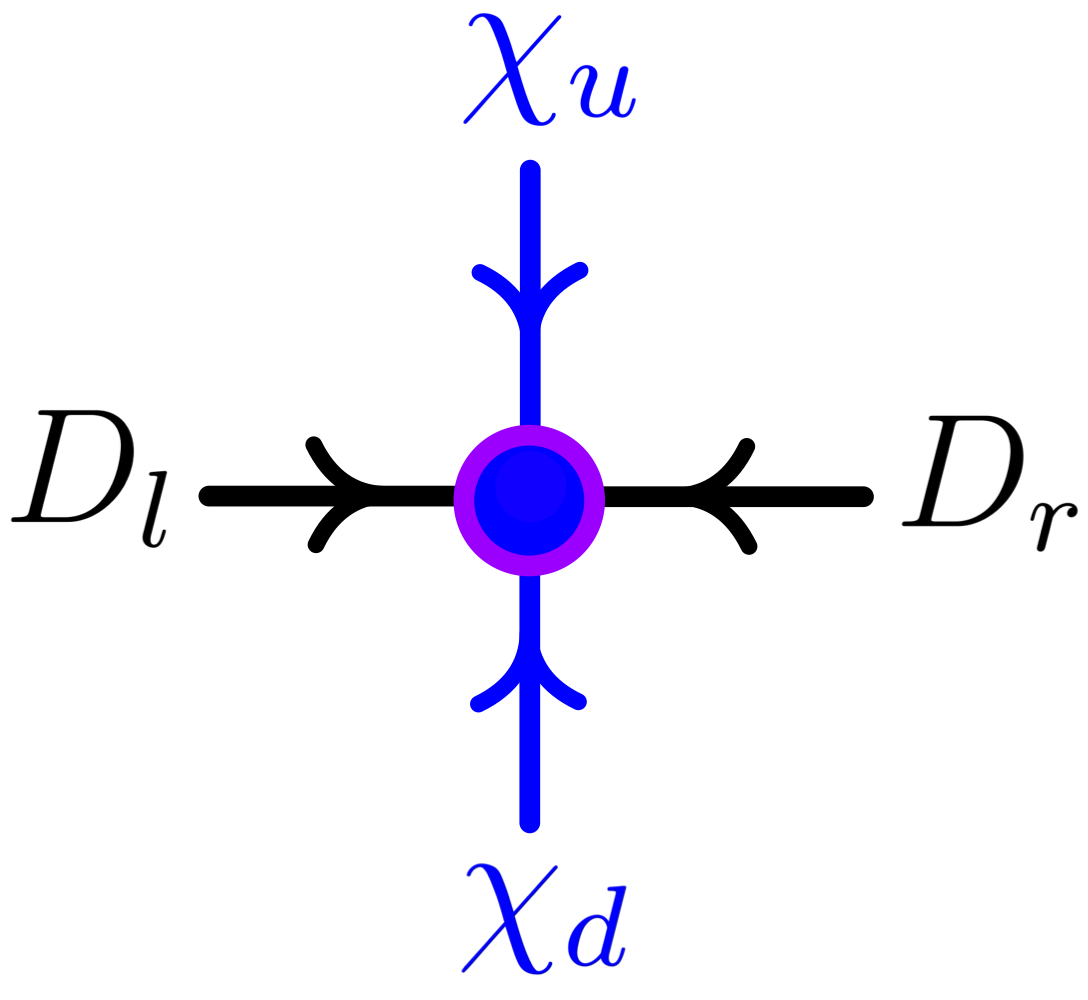
\includegraphics[height=1.9cm]{CC.png}}
	\:\text{ with }\:
	\raisebox{-0.5\height}{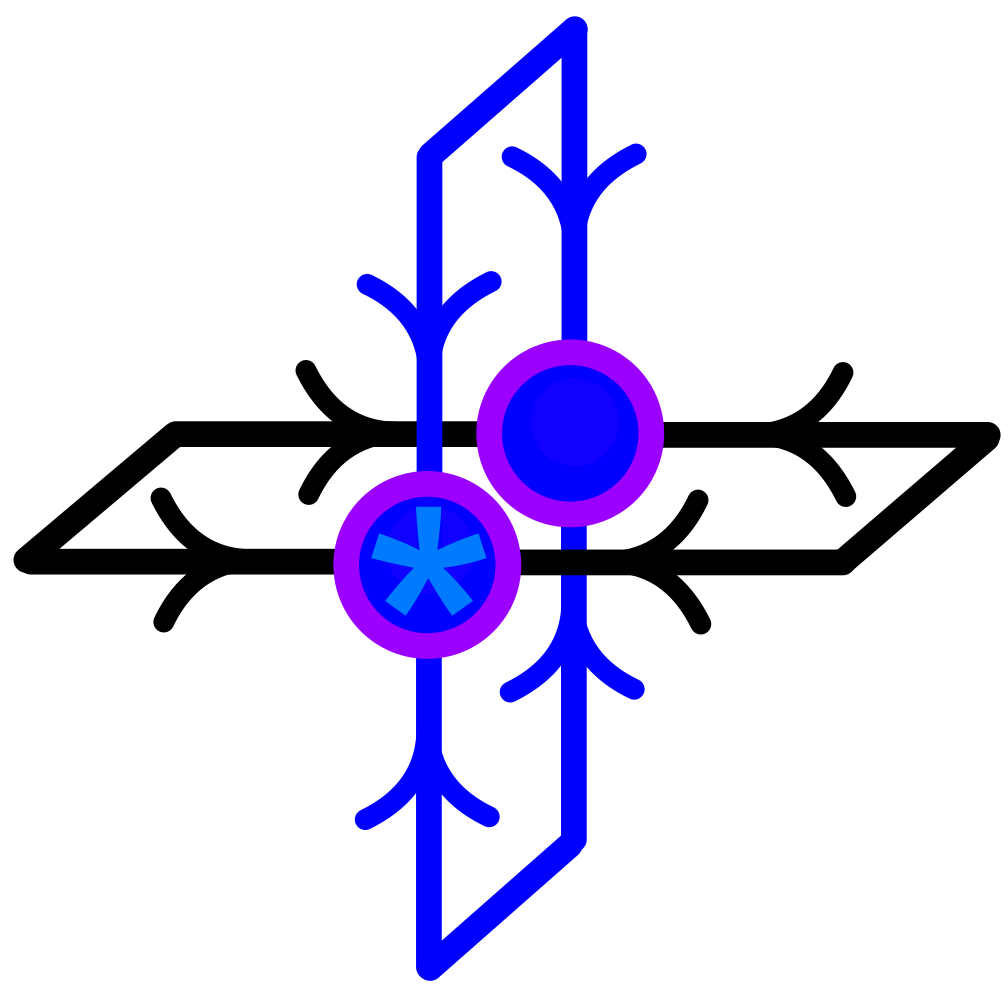
\includegraphics[height=1.5cm]{CC_contracted.png}}
	\:=\:
	1
	\hspace{0.2em},
\\
	C_D^{[n_x^c, n_y < n_y^c]} \label{eq:CD}
	&\:=\:
	\raisebox{-0.5\height}{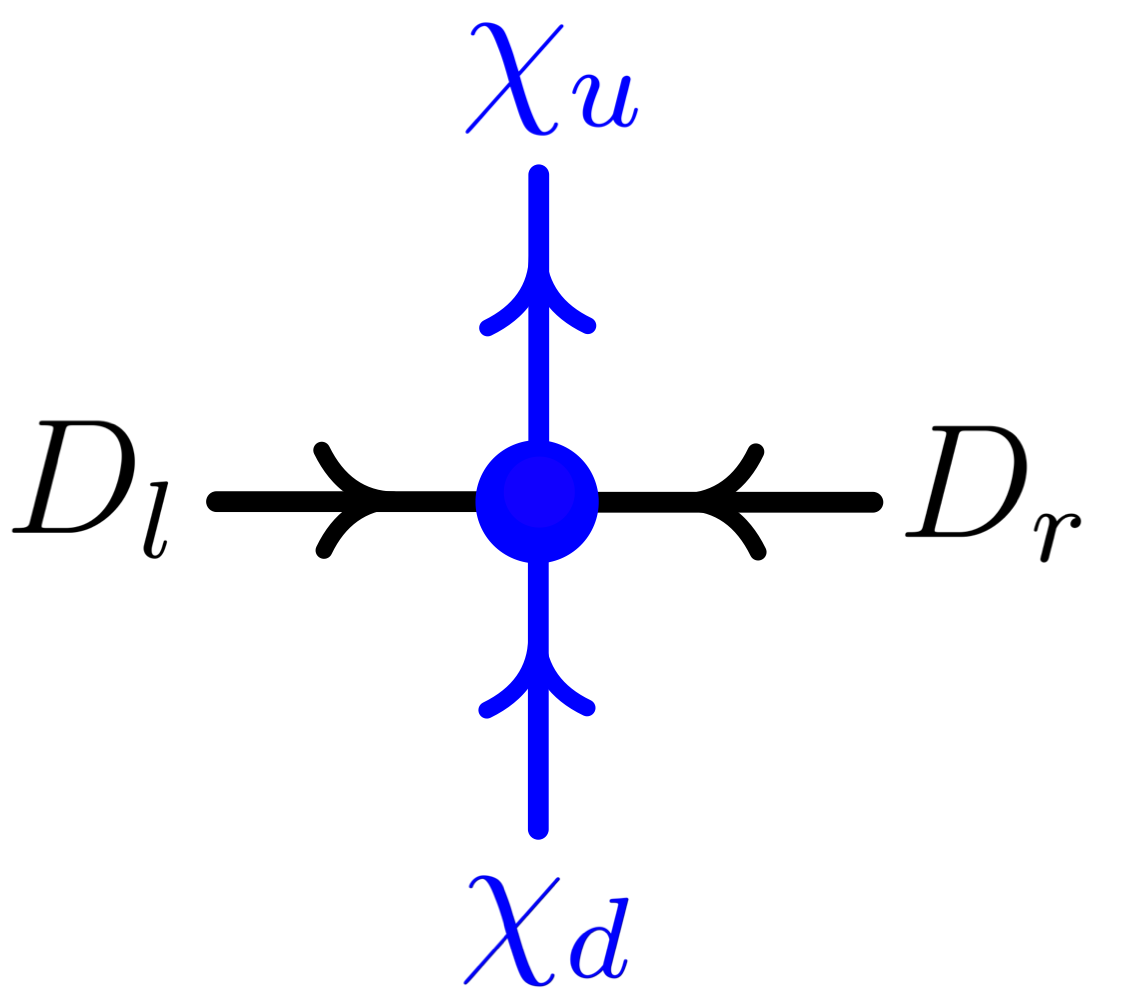
\includegraphics[height=1.9cm]{CD.png}}
	\:\text{ with }\:
	\raisebox{-0.5\height}{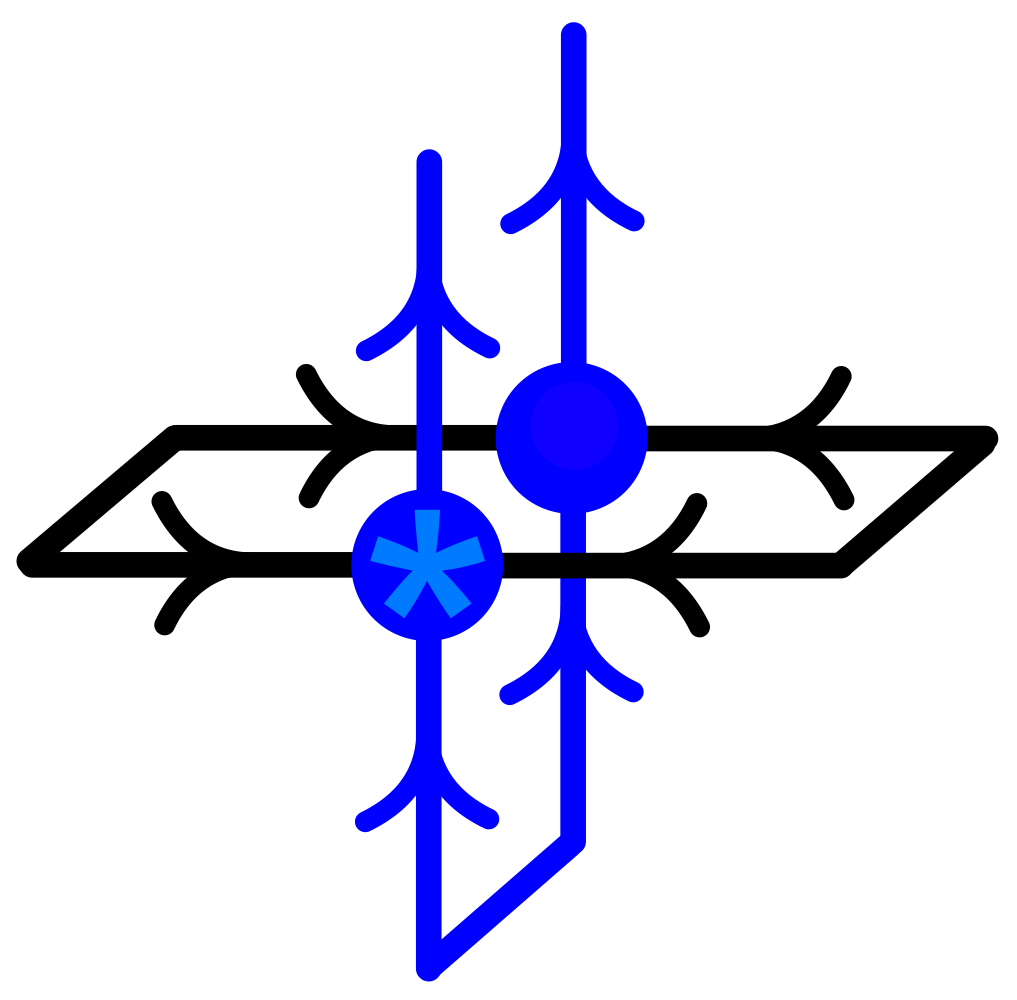
\includegraphics[height=1.5cm]{CD_contracted.png}}
	\:=\:
	\raisebox{-0.5\height}{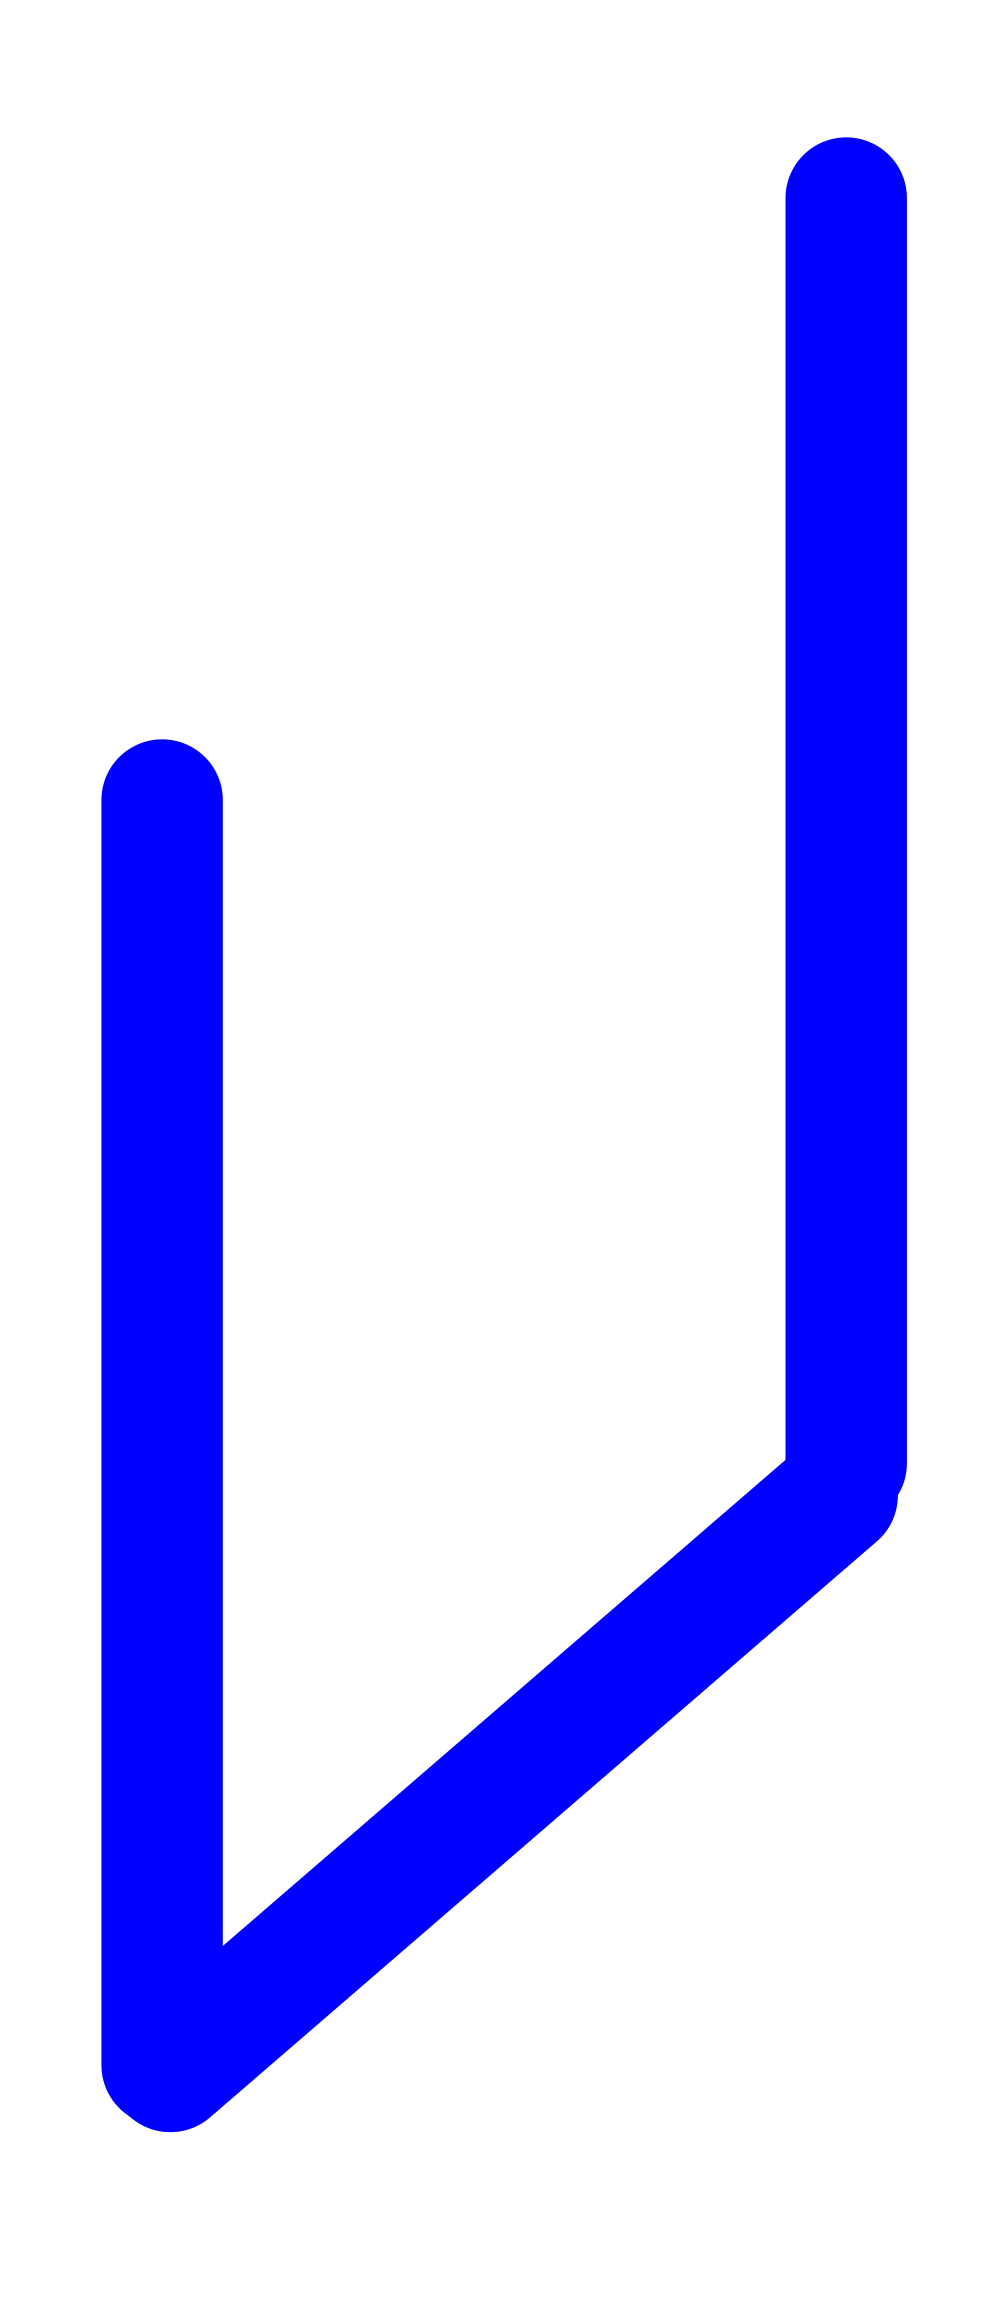
\includegraphics[height=0.9cm]{CD_id.png}}
	\hspace{0.2em}.
\end{align}
A set of tensors \eqref{eq:AL}--\eqref{eq:CD} defines an \textit{isometric projected entangled pair state} (isoPEPS):
\begin{equation} \label{eq:iso_peps}
	\ket{\psi(A_L, C, A_R)} 
	\:=\:
	\raisebox{-0.5\height}{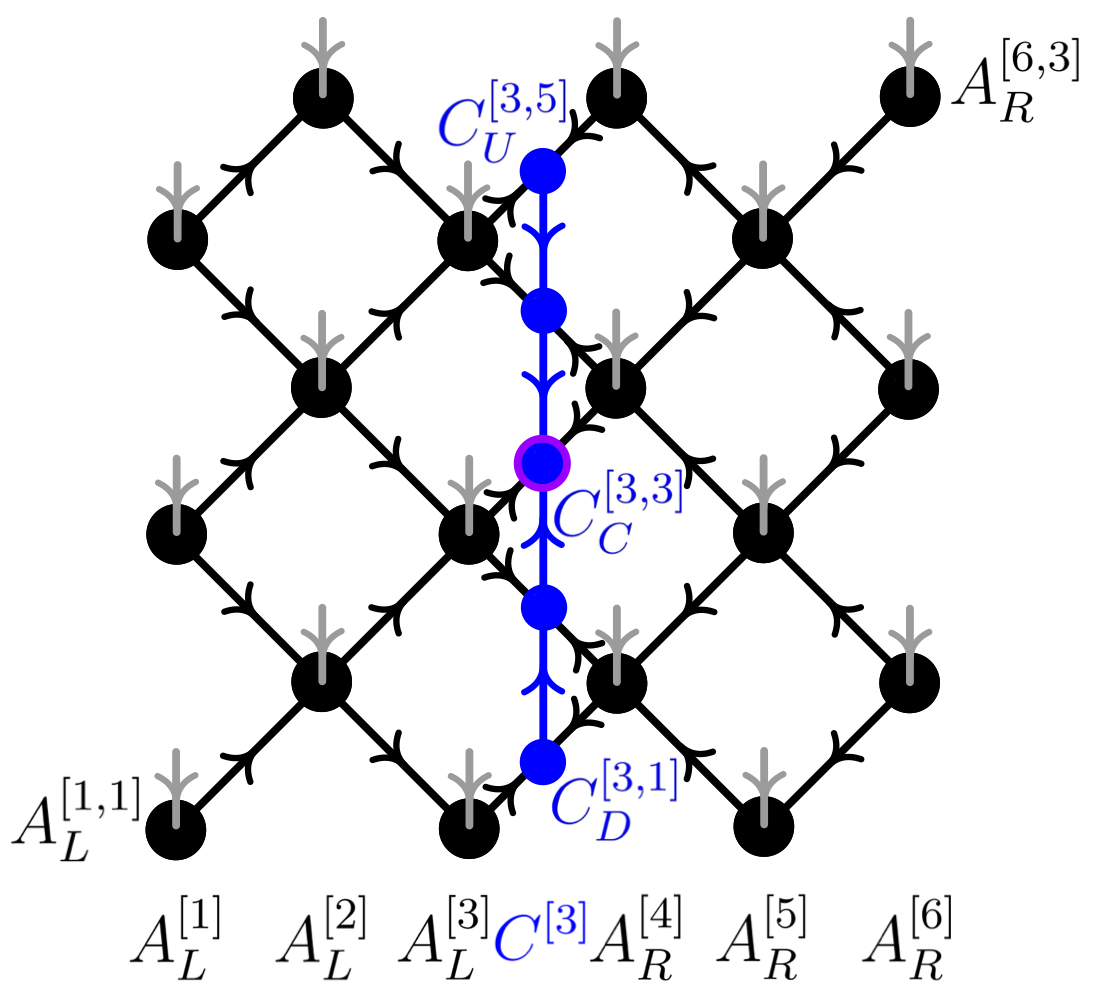
\includegraphics[height=5.5cm]{iso_peps.png}} .
\end{equation}
As in all diagrams in this chapter, we draw the diagonal lattice with $L_x = L_y = 3$ and $N = 2 L_x L_y = 18$ spins. For the orthogonality center we exemplarily choose $(n_x^c, n_y^c) = (3, 3)$. Note that we generally refer to both the indices $n_x^c$ and $(n_x^c, n_y^c)$, as well as the corresponding tensors $C^{[n_x^c]}$ and $C_C^{[n_x^c, n_y^c]}$, as the orthogonality column and orthogonality center, respectively. \\[1em]
\noindent In accordance with the physical MPS of chapter \ref{ch:mps}, we can interpret the orthogonality column $C^{[n_x^c]}$ as an MPS, with $d$ and $u$ the virtual legs and $rl$ the "physical" leg, where the quotation marks indicate that it is not an actual spin degree of freedom. We refer to this as a \textit{column MPS} (cMPS). In addition to the dimension constraints set by the boundaries and the isometric conditions (ingoing $\geq$ outgoing), we impose upper bounds $D_{\text{max}}$ and $\chi_{\text{max}, c}$ for the virtual lattice and column legs:
\begin{equation}
	D_{ld}, D_{lu}, D_{rd}, D_{ru}, D_l, D_r \leq D_{\text{max}}, \hspace{1em} \textcolor{blue}{\chi_d, \chi_u \leq \chi_{\text{max}, c}}.
\end{equation}
Within this thesis, we work with $D_{\text{max}} \leq 6$ and
\begin{equation}
\chi_{\text{max}, c} = 6 D_{\text{max}}. 
\end{equation}
To get an intuition for how the bond dimensions grow to their maximum value, we show a possible distribution for $D_{\text{max}} = 6$ and orthogonality column on the very right:
\begin{equation} \label{eq:iso_peps_right}
	\ket{\psi(A_L, C)} 
	\:=\:
	\begin{array}{cc}
	\raisebox{-0.5\height}{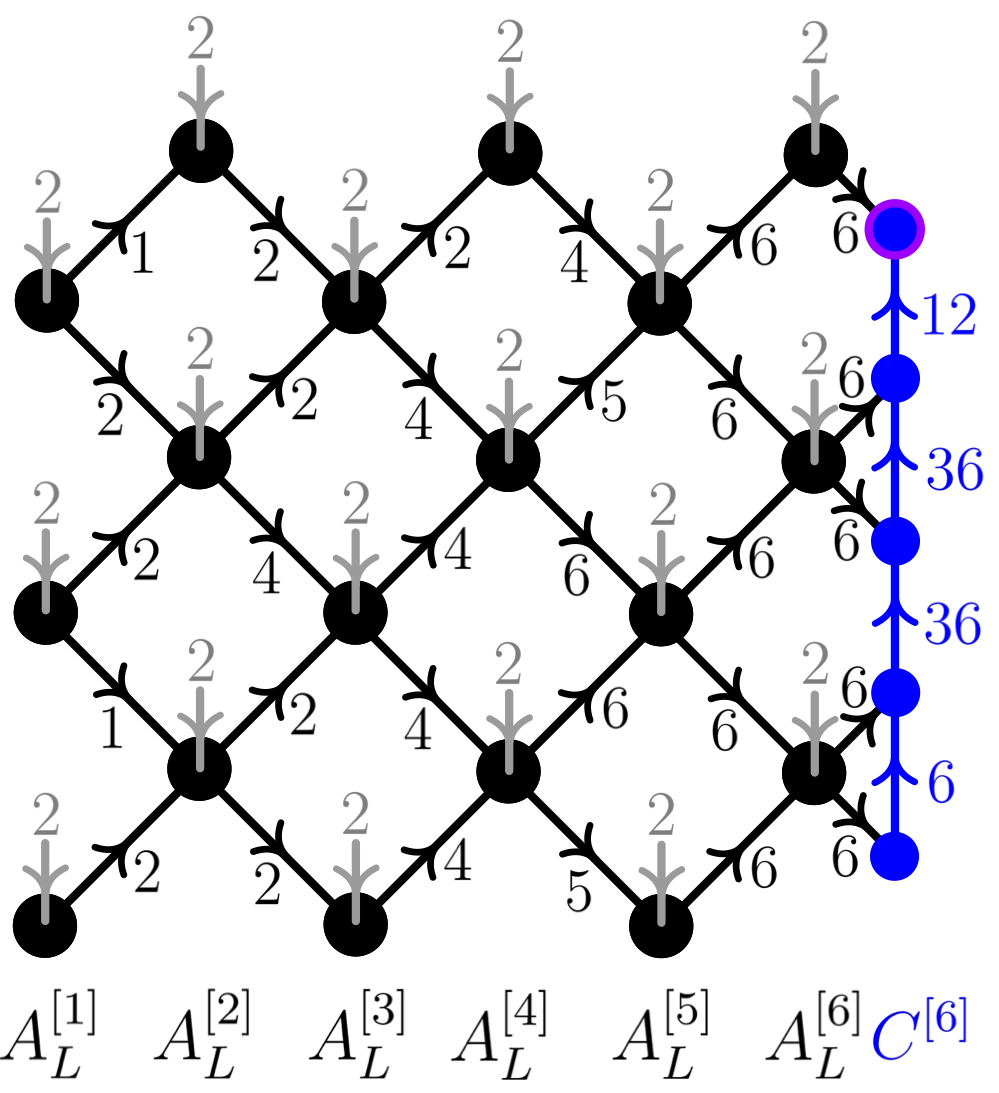
\includegraphics[height=5.5cm]{iso_peps_dimensions.png}} 
	&
	\begin{array}{l}
	D_{\text{max}} = 6 \\
	\textcolor{blue}{\chi_{\text{max}, c} = 36}
	\end{array}
	\end{array}.
\end{equation}

% yang baxter move
\noindent \underline{Yang-Baxter move} \\[0.5em]
\noindent The orthogonality center can be moved up/down error-free by performing a QR decomposition of $C_C$ and absorbing the normalized triangular matrix into the isometry above/below. Moving the orthogonality column left/right is a more involved, in general error-prone procedure. 
On the column level, it aims at solving the problem
\begin{equation} \label{eq:global_yb}
	C^{[n_x]} A_R^{[n_x + 1]} \approx \Tilde{A}_L^{[n_x + 1]} \Tilde{C}^{[n_x + 1]}.
\end{equation}
One way is to variationally minimize $\Vert C^{[n_x]} A_R^{[n_x + 1]} - \Tilde{A}_L^{[n_x + 1]} \Tilde{C}^{[n_x + 1]} \Vert_2$ by sweeping back and forth along the individual tensors $\Tilde{A}_L^{[n_x + 1, y]}$ and $\Tilde{C}^{[n_x + 1, n_y]}$ (for shift to the right). Achieving accuracy close to optimal while being much faster, we 
instead employ a sequential tripartite contraction-decomposition scheme, referred to as \textit{Yang-Baxter move} due to its diagrammatic resemblance to the Yang-Baxter equation:
\begin{equation} \label{eq:YB}
	\raisebox{-0.5\height}{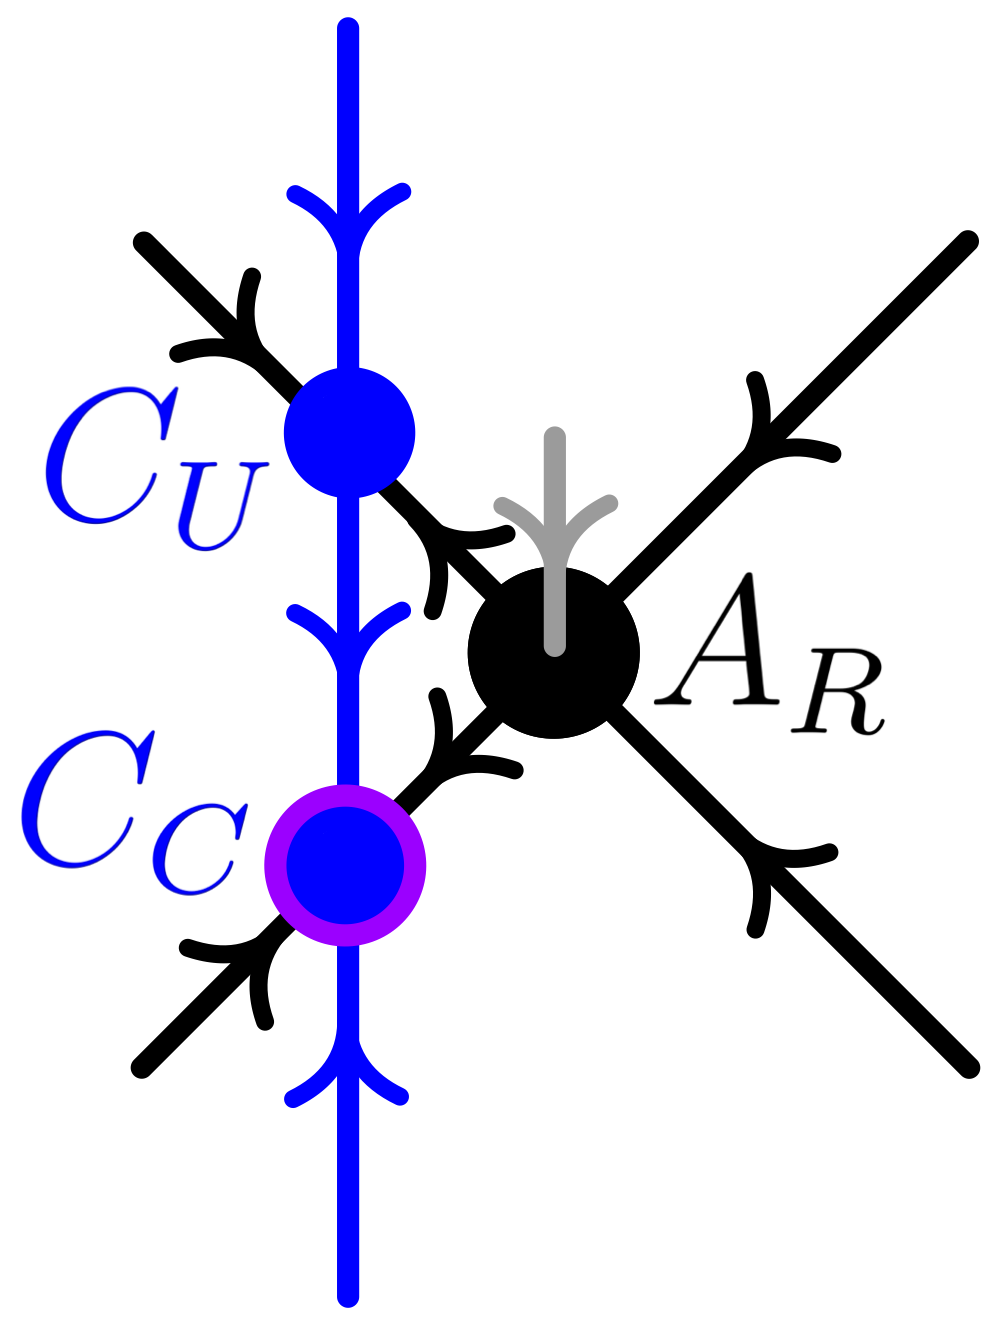
\includegraphics[height=2.5cm]{yb1.png}}
	\:\overset{\text{(YB1)}}{=}\:
	\raisebox{-0.5\height}{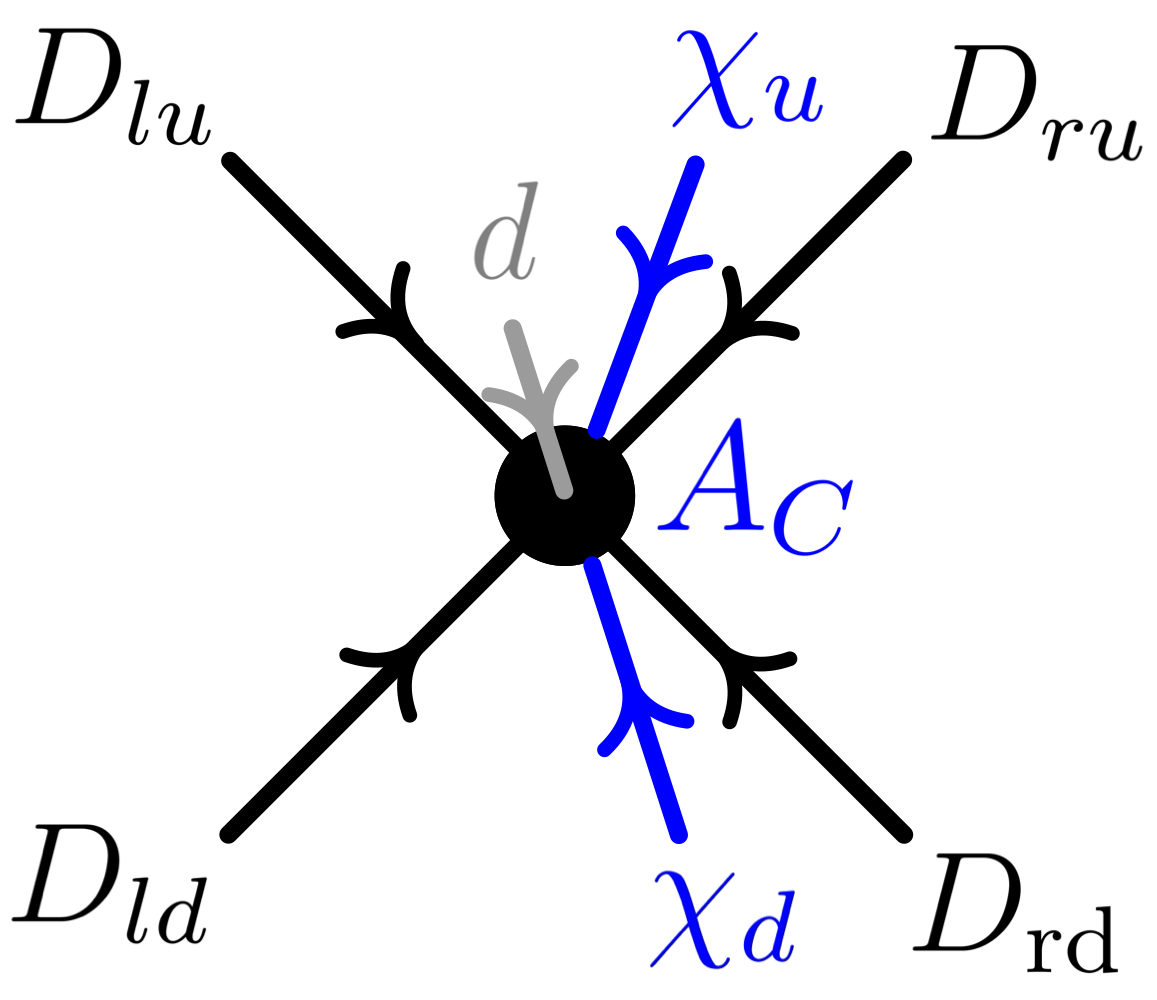
\includegraphics[height=2.5cm]{yb2.png}}
	\:\overset{\text{(YB2)}}{\approx}\:
	\raisebox{-0.5\height}{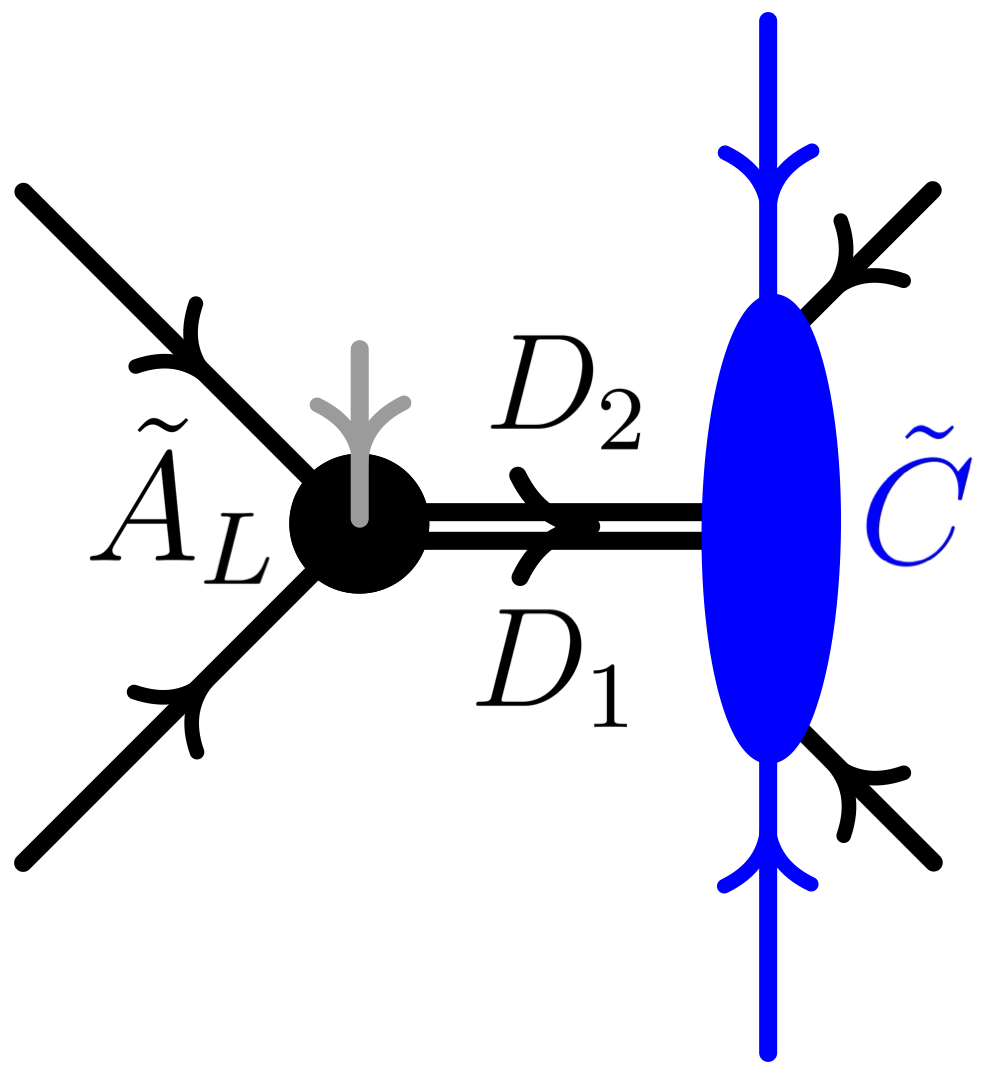
\includegraphics[height=2.5cm]{yb3.png}}
	\:\overset{\text{(YB3)}}{=}\:
	\raisebox{-0.5\height}{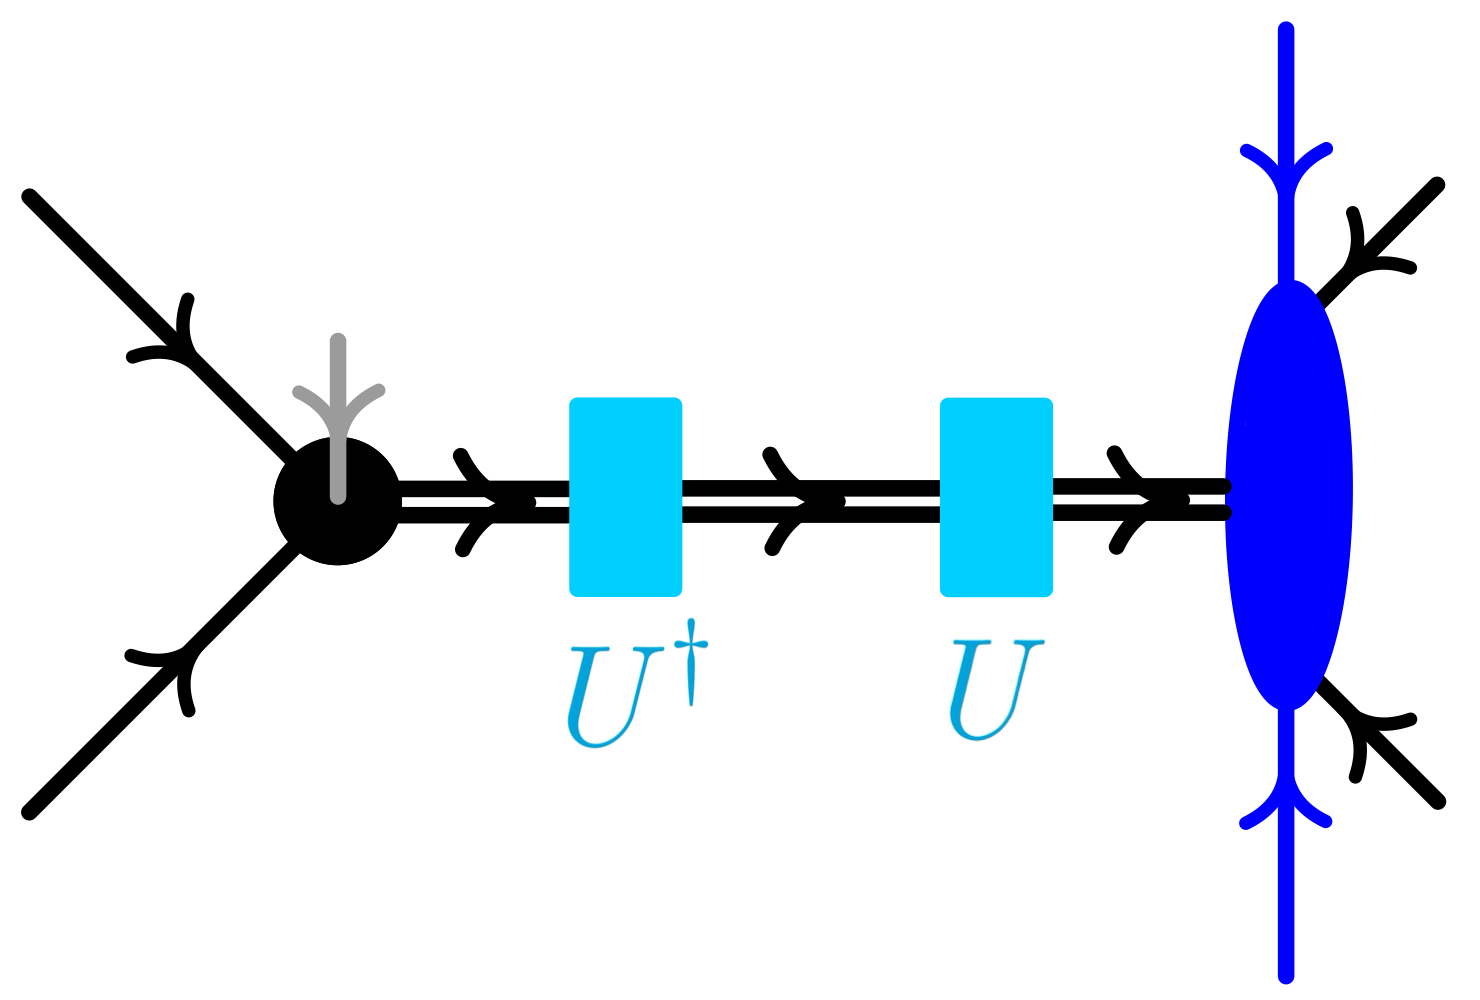
\includegraphics[height=2.5cm]{yb4.png}}
	\:\overset{\text{(YB4)}}{\approx}\:
	\raisebox{-0.5\height}{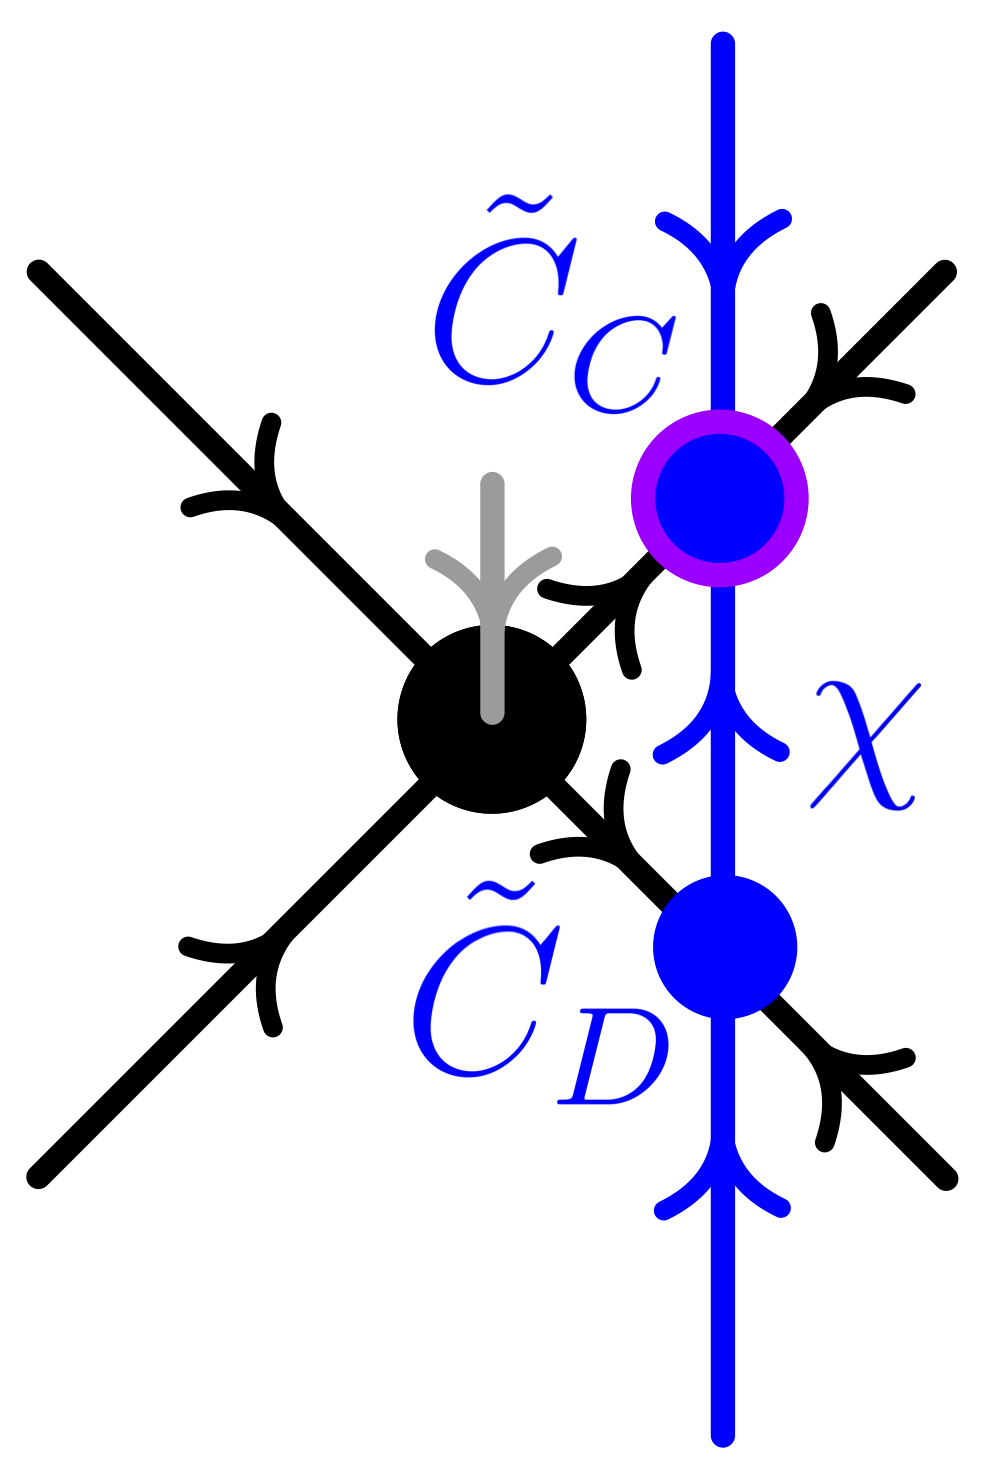
\includegraphics[height=2.5cm]{yb5.png}}
\end{equation}
\begin{itemize}
	\item[\text{(YB1)}] Contract $C_C$, $C_U$ and $A_R$ into a single normalized tensor $A_C$.
	\item[\text{(YB2)}] Perform a truncated SVD of $A_C \in \mathbb{C}^{(D_{ld} D_{lu} d) \times (\chi_d D_{rd} D_{ru} \chi_u)}$. Extract the new left isometry $\Tilde{A}_L$ and multiply singular value matrix and right isometry to a new center tensor $\Tilde{C}$:
	\begin{align}
	\begin{split}
		A_C \overset{\text{\textcolor{red}{t}SVD}}{\approx} \Tilde{A}_L \Tilde{C} 
		\:\text{ with }\: 
		&\Tilde{A}_L \in \mathbb{C}^{(D_{ld} D_{lu} d) \times \mathbb{D}}, 
		\Tilde{C} \in \mathbb{C}^{\mathbb{D} \times (\chi_d D_{rd} D_{ru} \chi_u)}, \\
		&\mathbb{D} = \text{min}(D_{ld} D_{lu} d, \chi_d D_{rd} D_{ru} \chi_u, \textcolor{red}{D_{\text{max}}^2}).
	\end{split}
	\end{align}
		Split the leg of dimension $\mathbb{D}$ into two legs of dimensions $D_1$, $D_2$ as evenly as possible under minimization of $\mathbb{D} - D_1 D_2 \geq 0$.
	\item[\text{(YB3)}] The decomposition $A_C \approx \Tilde{A}_L \Tilde{C}$ has the gauge freedom $\Tilde{A}_L \rightarrow \Tilde{A}_L U^{\dagger}$, $\Tilde{C} \rightarrow U \Tilde{C}$ for any unitary $U \in \mathbb{C}^{D_1D_2 \times D_1D_2}$. In anticipation of the truncated splitting \eqref{eq:tSVD_C_Tilde} of $\Tilde{C}$ into $\Tilde{C}_D$ and $\Tilde{C}_C$, we choose $U$ as their \textit{disentangler}. More precisely, we solve the variational problem
	\begin{equation} \label{eq:disentangling}
		\argmin_{U \in \text{GL}(D_1D_2, \mathbb{C})} \mathcal{L}(U \Tilde{C})
	\end{equation}
	for a cost function $\mathcal{L}$ whose minimization leads to a smaller truncation error 
	\begin{equation}
		\mathcal{E}_{\text{trunc}} (U \Tilde{C})
		= 
		\Vert U\Tilde{C} - {(\Tilde{C}_D)}_{[:, :\chi]} S_{[:\chi, :\chi]} V_{[:\chi, :]} \Vert_2 
		= 
		\left( \sum_{\mu > \chi} S_{\mu}^2 \right)^{1/2}.
	\end{equation} 
	In \cite{sappler2025diagonal} it was found that directly using $\mathcal{E}_{\text{trunc}}$ as cost function does not yield the smallest global error for shifting the whole orthonogonality column \eqref{eq:global_yb}. The best results were obtained with the Rényi-entropy 
	\begin{equation}
		\mathcal{R}_{\alpha}(U \Tilde{C}) 
		=
		\frac{1}{1 - \alpha} \log \tr_{u} \left[ \left(\tr_{d} \vert U \Tilde{C} ) (\overline{U \Tilde{C}} \vert \right)^{\alpha} \right] 
		= 
		\frac{1}{1 - \alpha} \log \left( \sum_{\mu} S_{\mu}^{2 \alpha} \right),
	\end{equation}
	for $\alpha = 1/2$. The partial traces are taken over all down, up legs of dimensions $D_1 \chi_d D_{rd}$, $D_{ru} \chi_u D_2$. Note that $\mathcal{E}_{\text{trunc}}$ is upper bounded by $\mathcal{R}_{\alpha}$ for all $\alpha < 1$. For a detailed description of the Riemannian Trust-Region Method (TRM), used to solve \eqref{eq:disentangling} for $\mathcal{R}_{\alpha=1/2}$, we refer the reader to \cite{sappler2025diagonal, lin2022efficient}. 
	\item[\text{(YB4)}] Split $\Tilde{C} \in \mathbb{C}^{(D_1 \chi_d D_{rd}) \times (D_{ru} \chi_u D_2)}$ into down isometric $\Tilde{C}_D$ and normalized $\Tilde{C}_C$ via truncated SVD:
	\begin{align} \label{eq:tSVD_C_Tilde}
	\begin{split}
		\Tilde{C} \overset{\text{\textcolor{red}{t}SVD}}{\approx} \Tilde{C}_D \Tilde{C}_C
		\:\text{ with }\: 
		&\Tilde{C}_D \in \mathbb{C}^{(D_1 \chi_d D_{rd}) \times \chi}, 
		\Tilde{C}_C \in \mathbb{C}^{\chi \times (D_{ru} \chi_u D_2)}, \\
		&\chi = \text{min}(D_1 \chi_d D_{rd}, D_{ru} \chi_u D_2, \textcolor{red}{\chi_{\text{max},c}}).
	\end{split}
	\end{align}
\end{itemize} 
Starting from $C_C$ at $(n_x, 1)$, we can shift the whole orthogonality column to the right and end up with $\Tilde{C}_C$ at $(n_x+1, 2L_y - 1)$
by repeating (YB1)--(YB4) $L_y$ times, each (apart from the last one) followed by moving $C_C$ up to the next site. Depending on the parity of $n_x$, the decomposition at the very bottom or top reduces to a bipartition, so steps (YB3) and (YB4) are omitted in that case. To instead move the center from top to bottom, i.e. from $(n_x, 2L_y - 1)$ to $(n_x+1, 1)$, one just has to reverse the direction of the final truncated SVD in (YB4). Since the respective shifts to the left result from mirroring along the y-axis, they don't have to be implemented separately. \\


% BOUNDARY COMPRESSION
\newpage
\section{Boundary compression} \label{sec:bc}

% column MPO hamiltonian
\noindent \underline{Column MPO Hamiltonian} \\[0.5em]
We can write any Hamiltonian $H = H^{\dagger} \in \mathbb{C}^{d^{2L_xL_y} \times d^{2L_xL_y}}$ with nearest-neighbor interactions as a sum of zig-zag MPOs $h^{[n_x, n_x +1]}$ that act nontrivially only on two adjacent columns of physical sites:
\begin{align} \label{eq:column_mpo}
\begin{split}
	&H = \sum_{n_x = 1}^{2 L_x - 1} 
	\mathbbm{1}^{[1]}
	\otimes \cdots \otimes 
	\mathbbm{1}^{[n_x-1]}
	\otimes 
	h^{[n_x, n_x +1]}
	\otimes 
	\mathbbm{1}^{[n_x+2]}
	\otimes \cdots \otimes 
	\mathbbm{1}^{[2L_x]}, \\
	& h^{[n_x, n_x +1]} = \raisebox{-0.5\height}{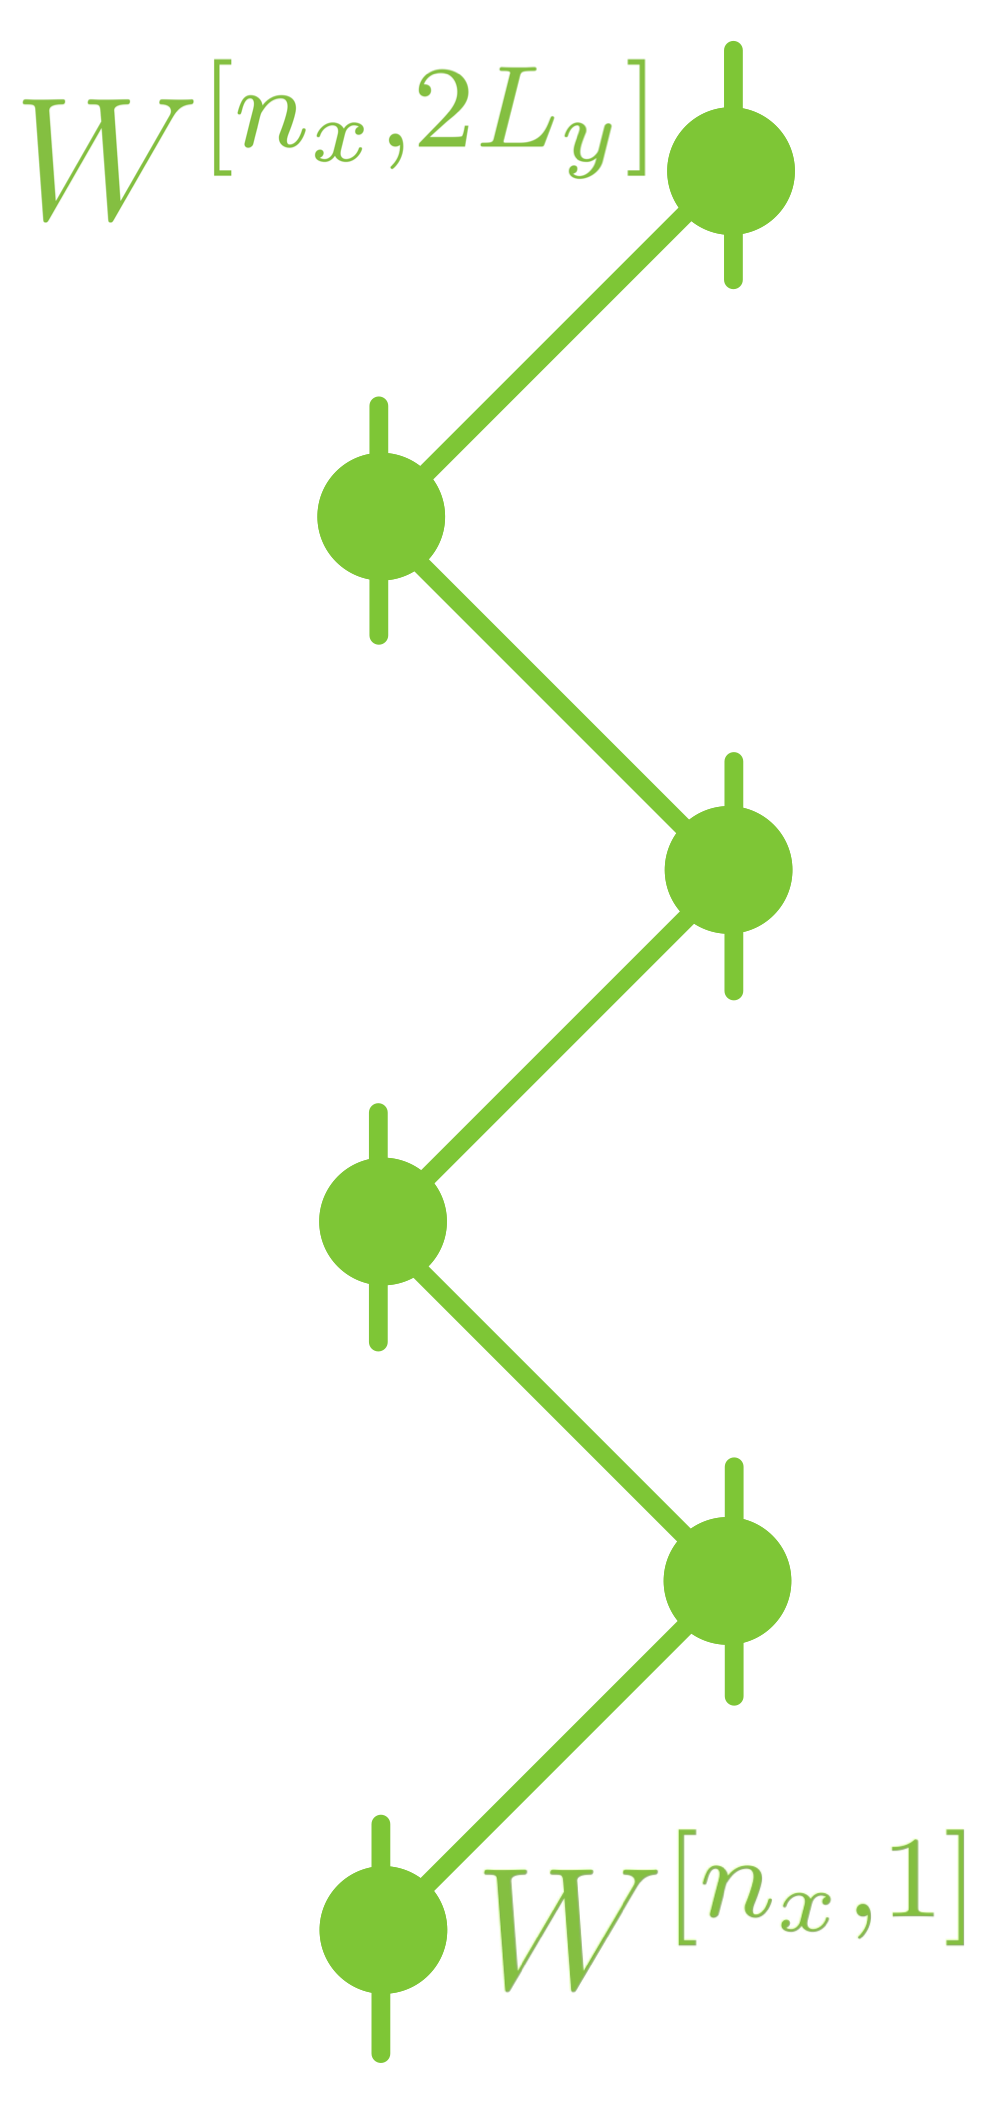
\includegraphics[height=4.5cm]{h.png}} \text{ for } n_x \text{ odd }, \:\:
	\raisebox{-0.5\height}{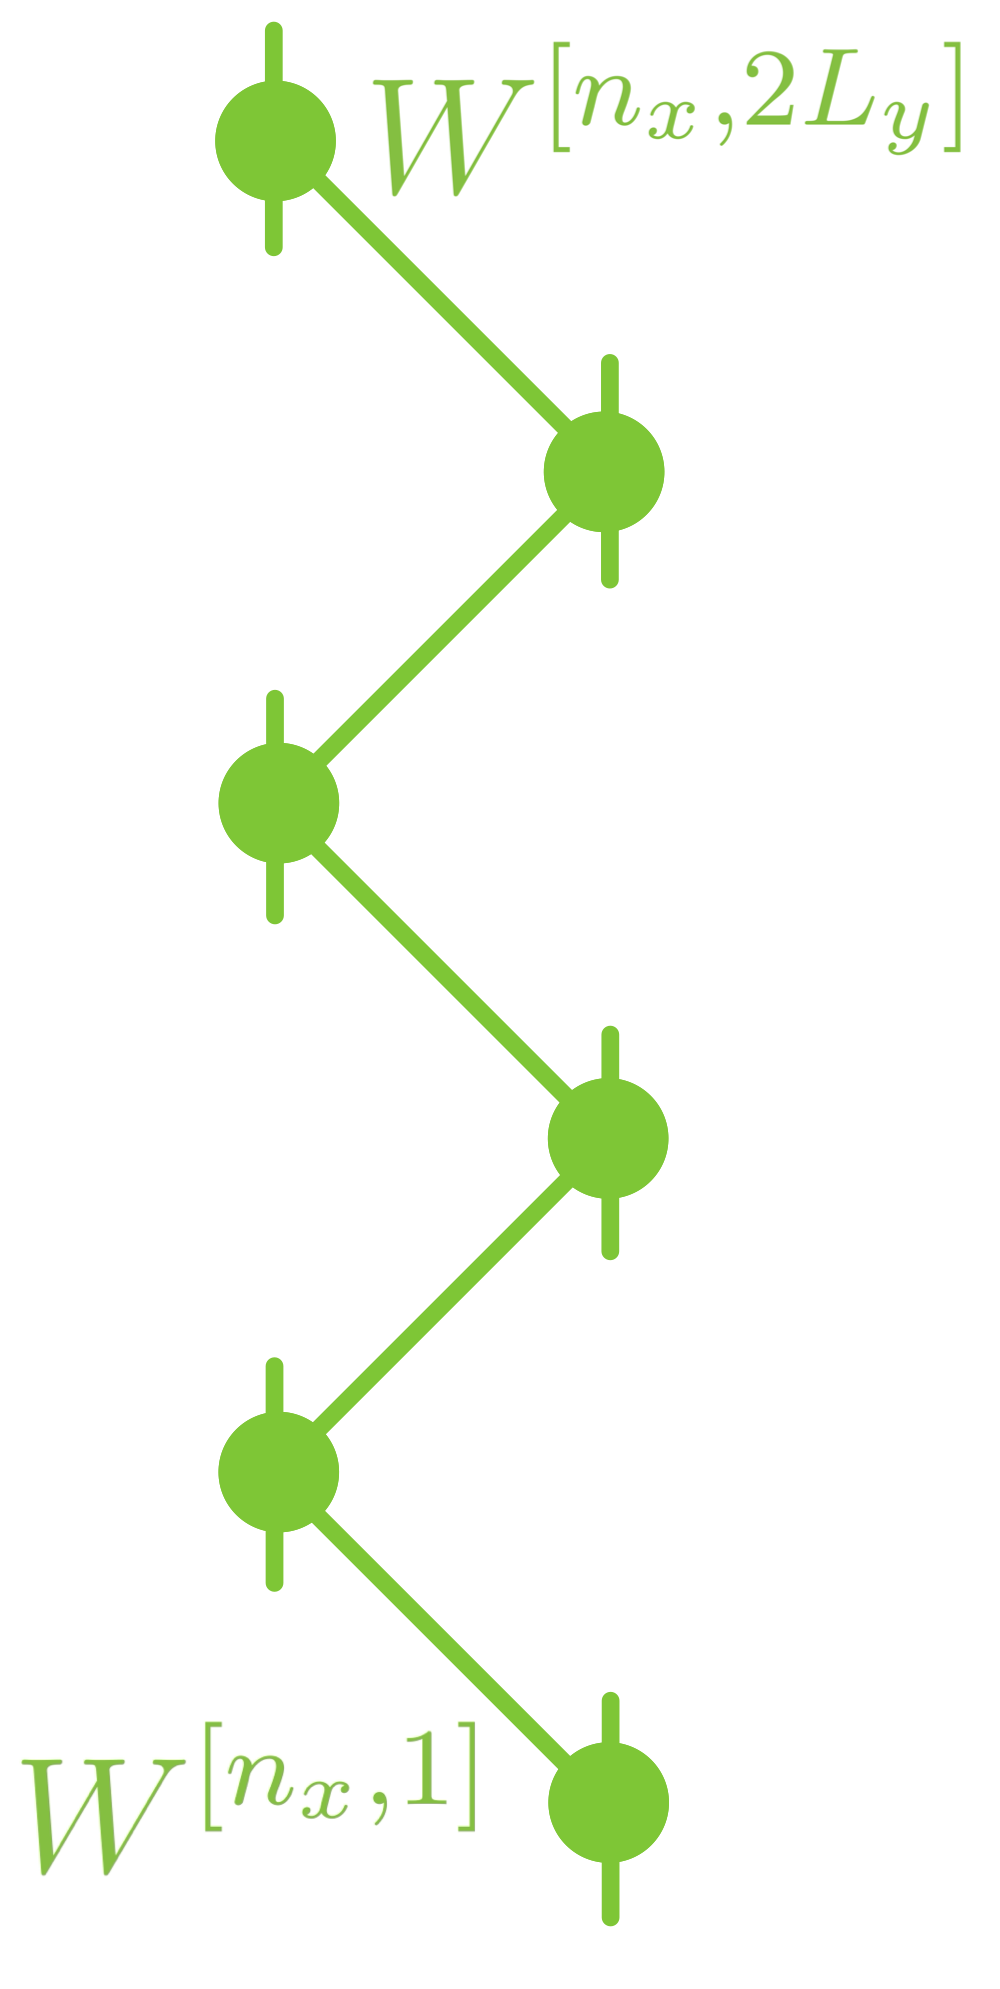
\includegraphics[height=4.5cm]{h_even.png}} \text{ for } n_x \text{ even }.
\end{split}
\end{align}
For the TFI model \eqref{eq:tfi_hamiltonian} with OBC, the MPO tensors $W^{[n_x, n_y]}$ are given by
\begin{equation} \label{eq:tfi_column_mpo}
	\overset{\raisebox{0.5em}{$W^{[n_x, 1]}$}}{\begin{pmatrix} \mathbbm{1} & \sigma^x & -g^{[n_x, 1]} \sigma^z \end{pmatrix}}, 
	\hspace{0.5em}
	\overset{\raisebox{0.5em}{$W^{[n_x, 2]}, \ldots, W^{[n_x, 2L_y-1]}$}}{\begin{pmatrix}  \mathbbm{1} & \sigma^x & -g^{[n_x, n_y]} \sigma^z \\ 0 & 0 & -J \sigma^x \\ 0 & 0 & \mathbbm{1} \end{pmatrix}}, 
	\hspace{0.5em}
	\overset{\raisebox{0.5em}{$W^{[n_x, 2L_y]}$}}{\begin{pmatrix} -g^{[n_x, 2L_y]} \sigma^z \\ -J \sigma^x \\ \mathbbm{1} \end{pmatrix}}.
\end{equation}
For all spins that are involved in two MPOs (all except the leftmost and rightmost), the transverse field strengths have to be halved:
\begin{equation}
	g^{[n_x, n_y]} = 
	\begin{cases}
		g & \text{ if } n_x = 1, n_y \text{ odd} \\
		g & \text{ if } n_x = 2L_x-1, n_y \text{ even} \\
		g/2 & \text{ else }
	\end{cases}
	.
\end{equation}

\vspace*{2em}

\noindent For an isoPEPS \eqref{eq:iso_peps}, we now develop two different ways to compute the expectation value $E$ of a Hamiltonian \eqref{eq:column_mpo}. Without performing any contractions, it has the diagrammatic representation
\begin{equation}\label{eq:E}
	E \:=\:
	\raisebox{-0.5\height}{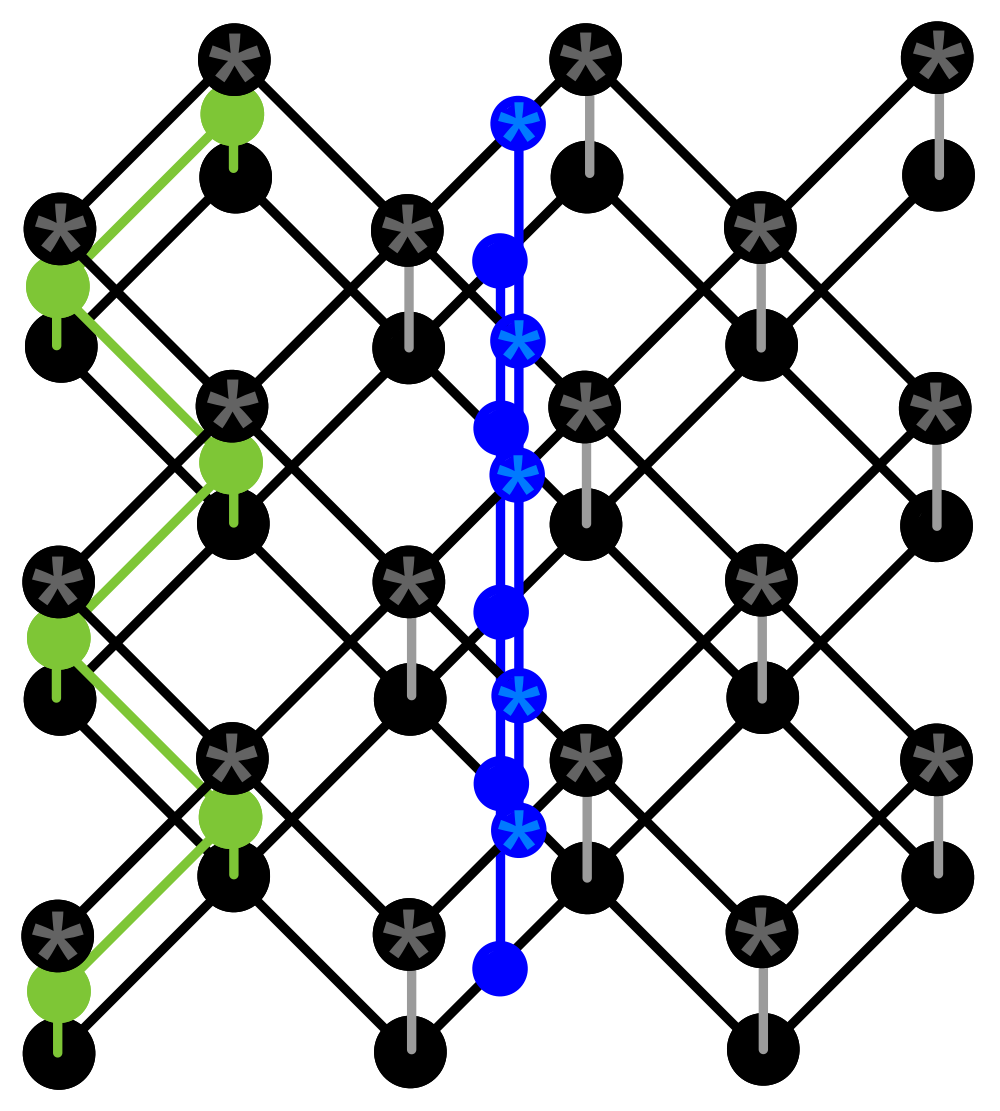
\includegraphics[height=3cm]{E1.png}}
	\:+\:
	\raisebox{-0.5\height}{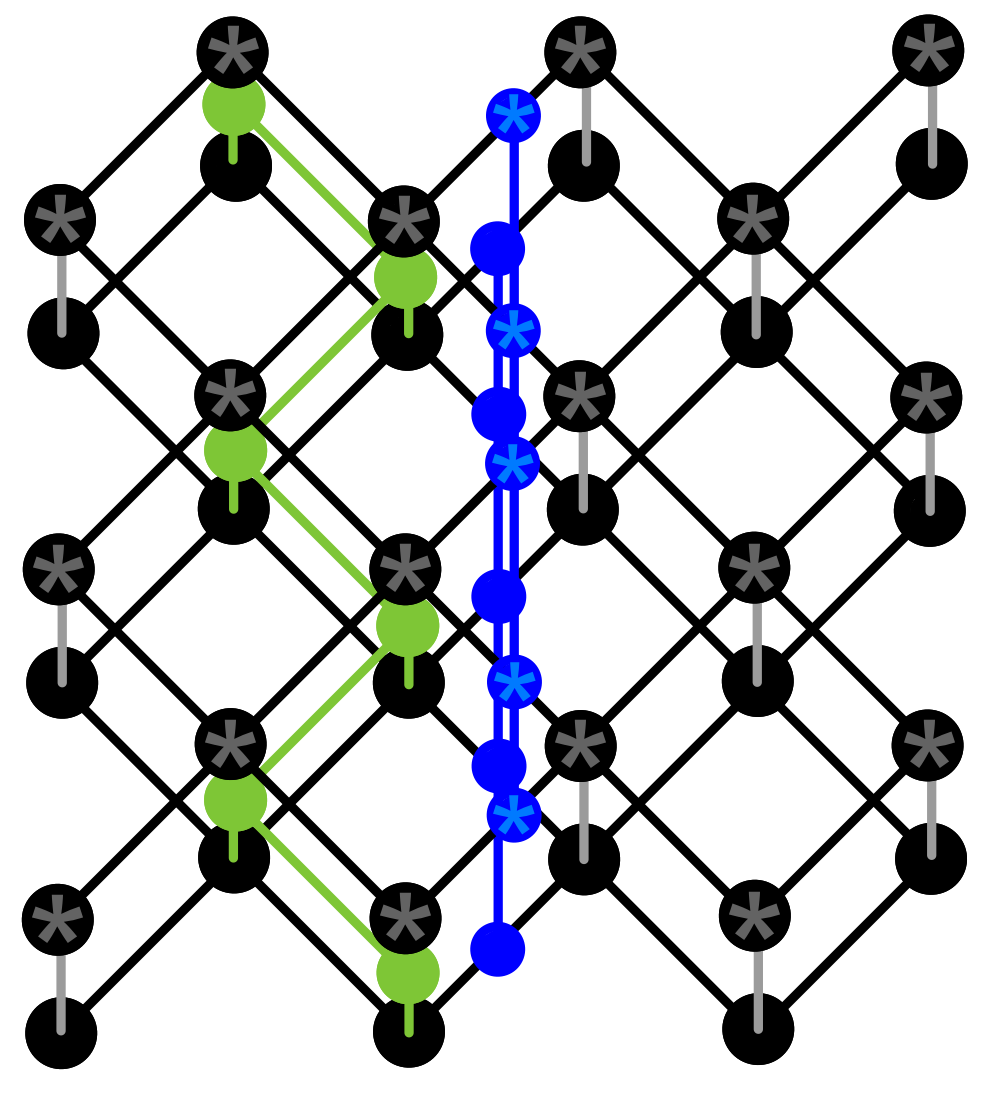
\includegraphics[height=3cm]{E2.png}}
	\:+\:
	\raisebox{-0.5\height}{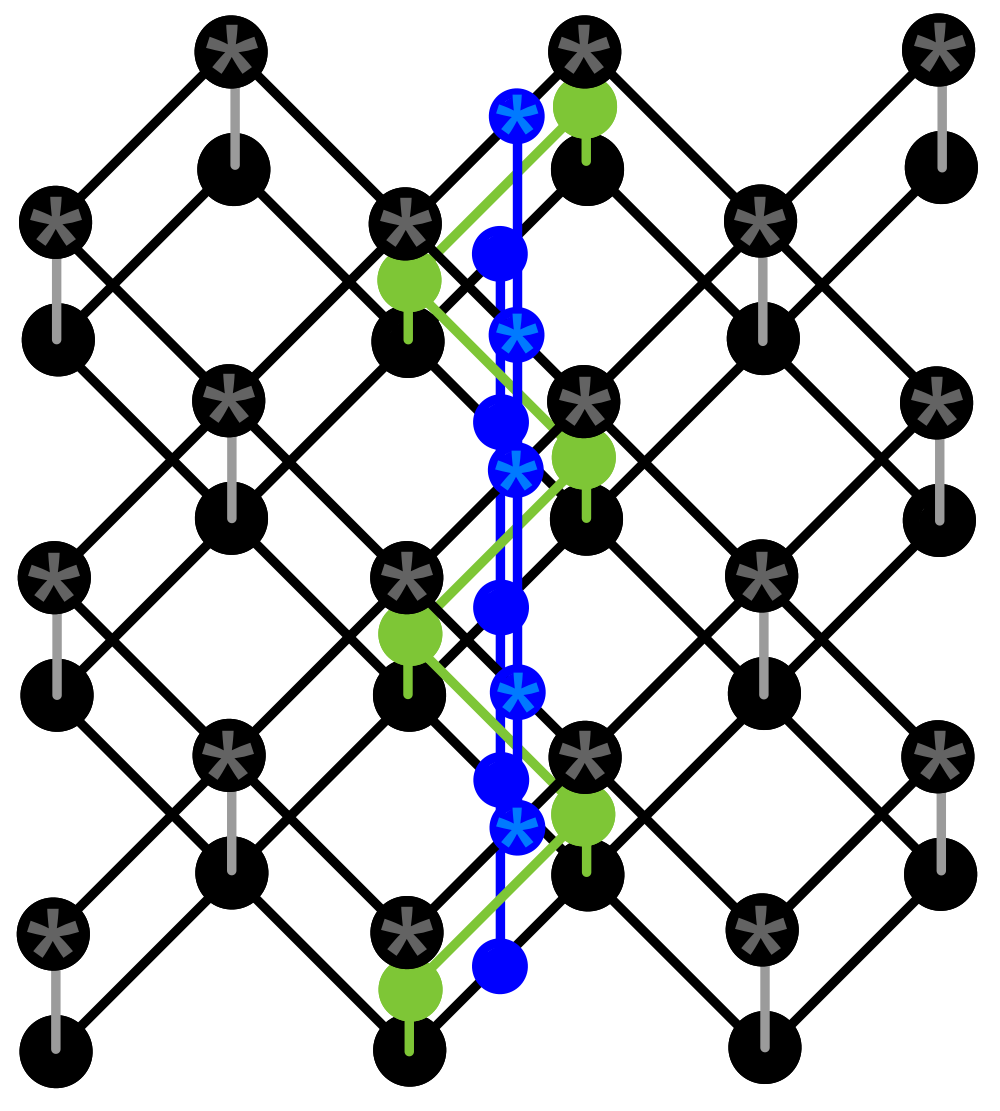
\includegraphics[height=3cm]{E3.png}} 
	\:+\:
	\raisebox{-0.5\height}{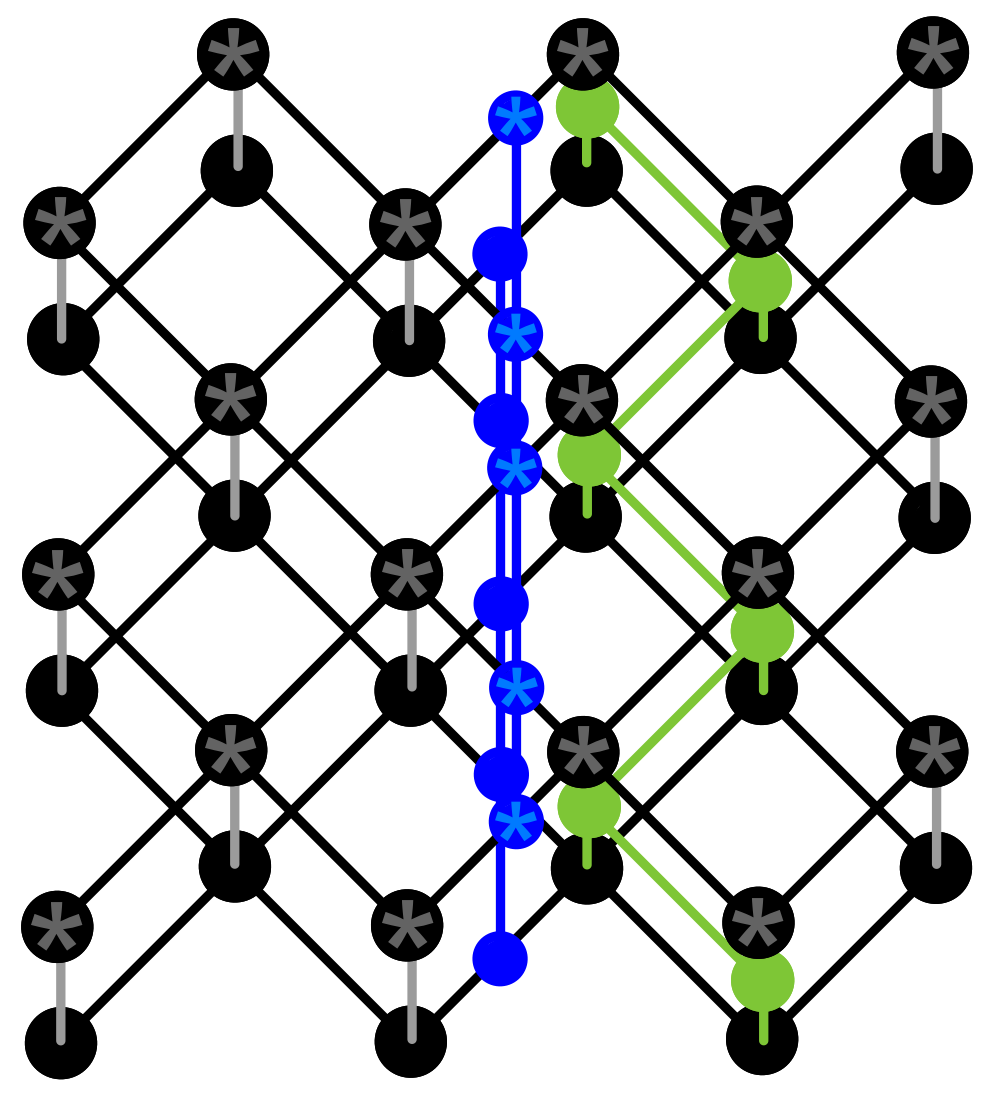
\includegraphics[height=3cm]{E4.png}}
	\:+\:
	\raisebox{-0.5\height}{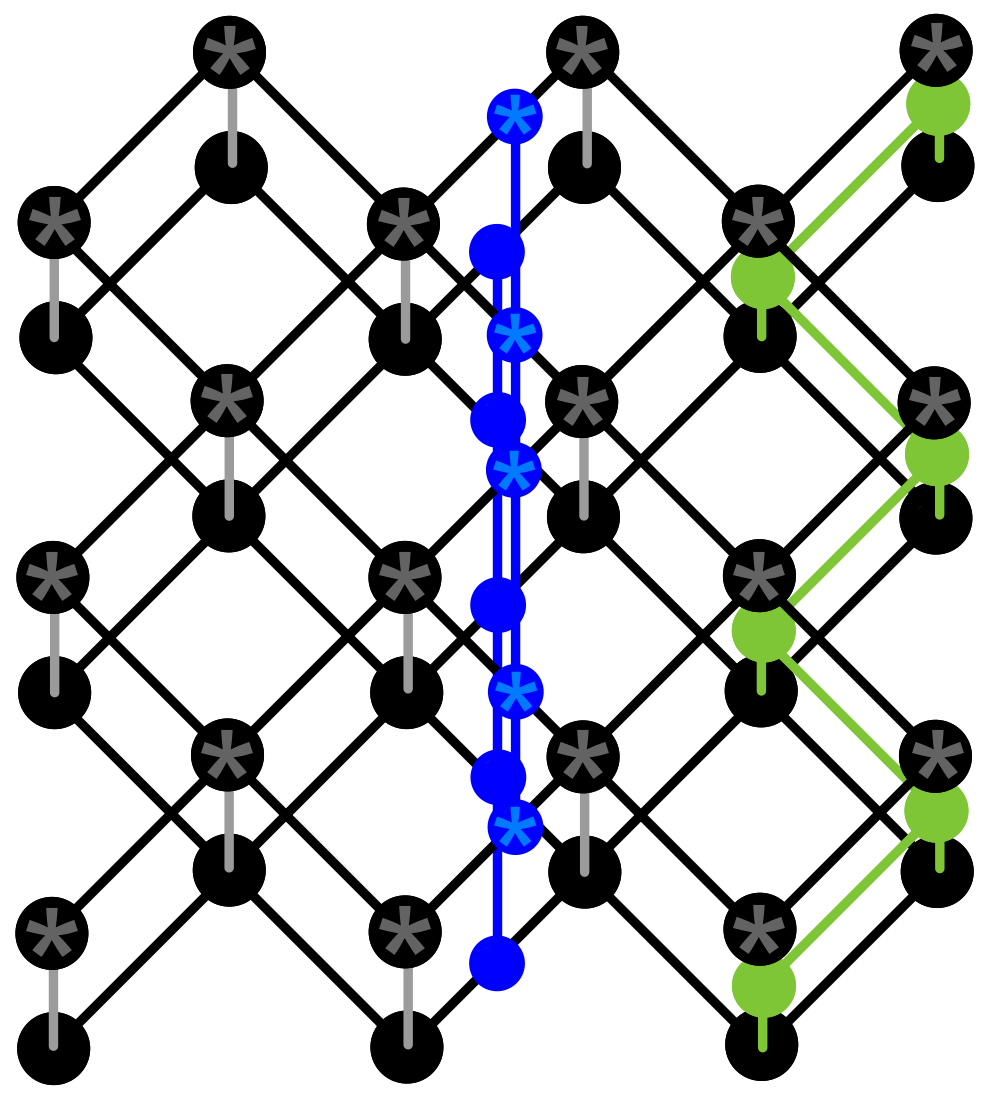
\includegraphics[height=3cm]{E5.png}}
	\:.
\end{equation}


\newpage
\noindent 1) Yang-Baxter energy \\[0.5em]
\noindent One way to compute \eqref{eq:E} is to move the orthogonality column with Yang-Baxter moves right next to every column MPO in the sum, and to use the isometry condition for all $A_L$, $A_R$ tensors on which the MPO does not act:
\begin{equation}\label{eq:E_YB}
	E_{\text{YB}} 
	\:=\: \sum_{n_x=1}^{2L_x-1}
	\begin{array}{c}
	\raisebox{-0.5\height}{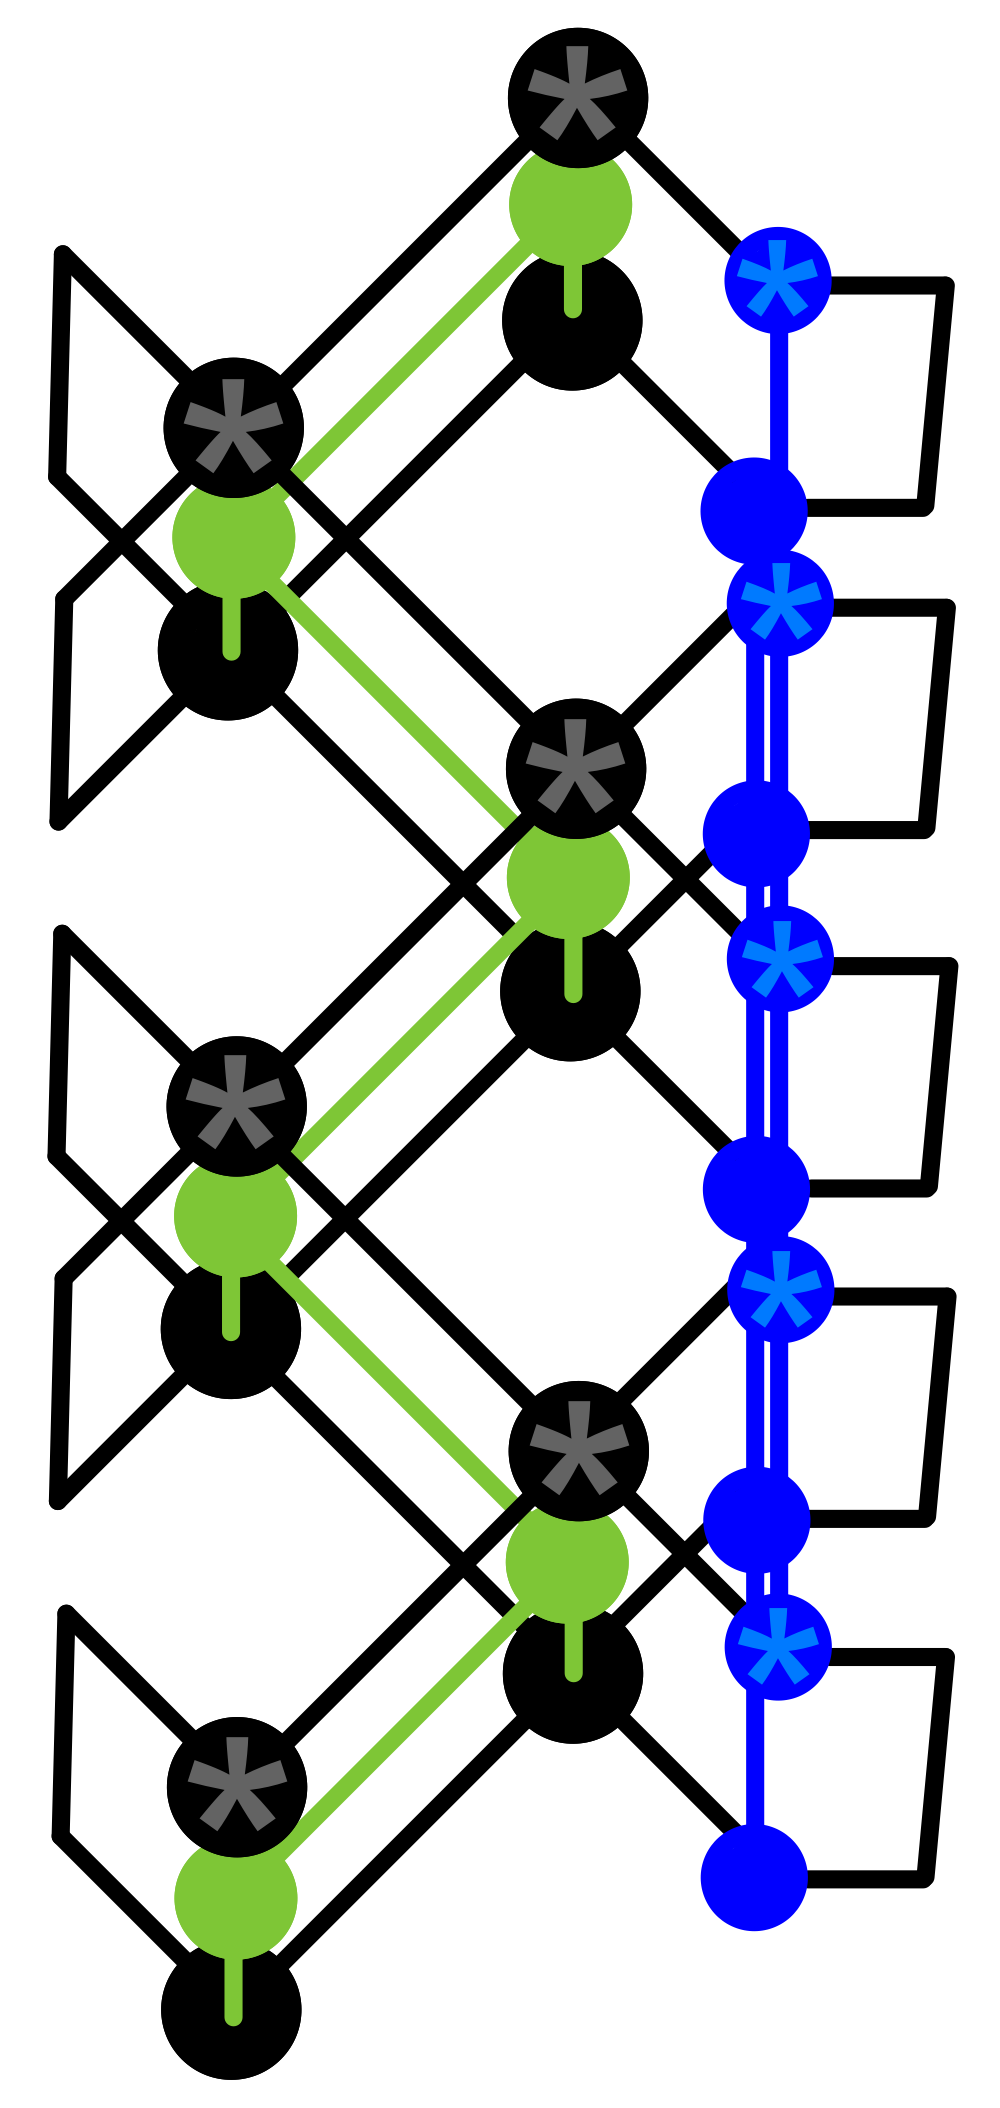
\includegraphics[height=4.5cm]{E_YB.png}} \\
	\left( 
	\begin{array}{c}
	\overline{A}_L^{[n_x]} \overline{A}_L^{[n_x+1]} \\
	\textcolor{LimeGreen}{h^{[n_x, n_x +1]}} \\
	A_L^{[n_x]} A_L^{[n_x+1]}
	\end{array}
	\middle\vert 
	\begin{array}{c}
	\textcolor{blue}{\overline{C}^{[n_x +1]}} \\
	\textcolor{blue}{C^{[n_x +1]}}
	\end{array}
	\middle\vert
	\mathbbm{1}
	\right)
	\end{array}
	\:.
\end{equation}

\vspace*{2em}

\noindent 2) Boundary compression energy \\[0.5em]
\noindent In section \ref{sec:dmrg2}, we want to take the derivative of \eqref{eq:E} with respect to tensors on the orthogonality column in order to find the ground state. This requires an alternative computation of the energy, where we keep the orthogonality column fixed at $n_x^c$. We additively summarize all terms where $h^{[n_x, n_x+1]}$ acts left ($n_x < n_x^c$) and right ($n_x > n_x^c$) of the orthogonality column into environments $L_h^{[n_x^c]}$ and $R_h^{[n_x^c+1]}$, respectively. They are defined more precisely below. The third contribution comes from $h^{[n_x^c, n_x^c+1]}$ acting on $A_L^{[n_x^c]}$ and $A_R^{[n_x^c+1]}$, which enclose the orthogonality column:
\begin{equation}\label{eq:E_bc}
	E_{\text{bc}} 
	\:=\:
	\begin{array}{c}
	\raisebox{-0.5\height}{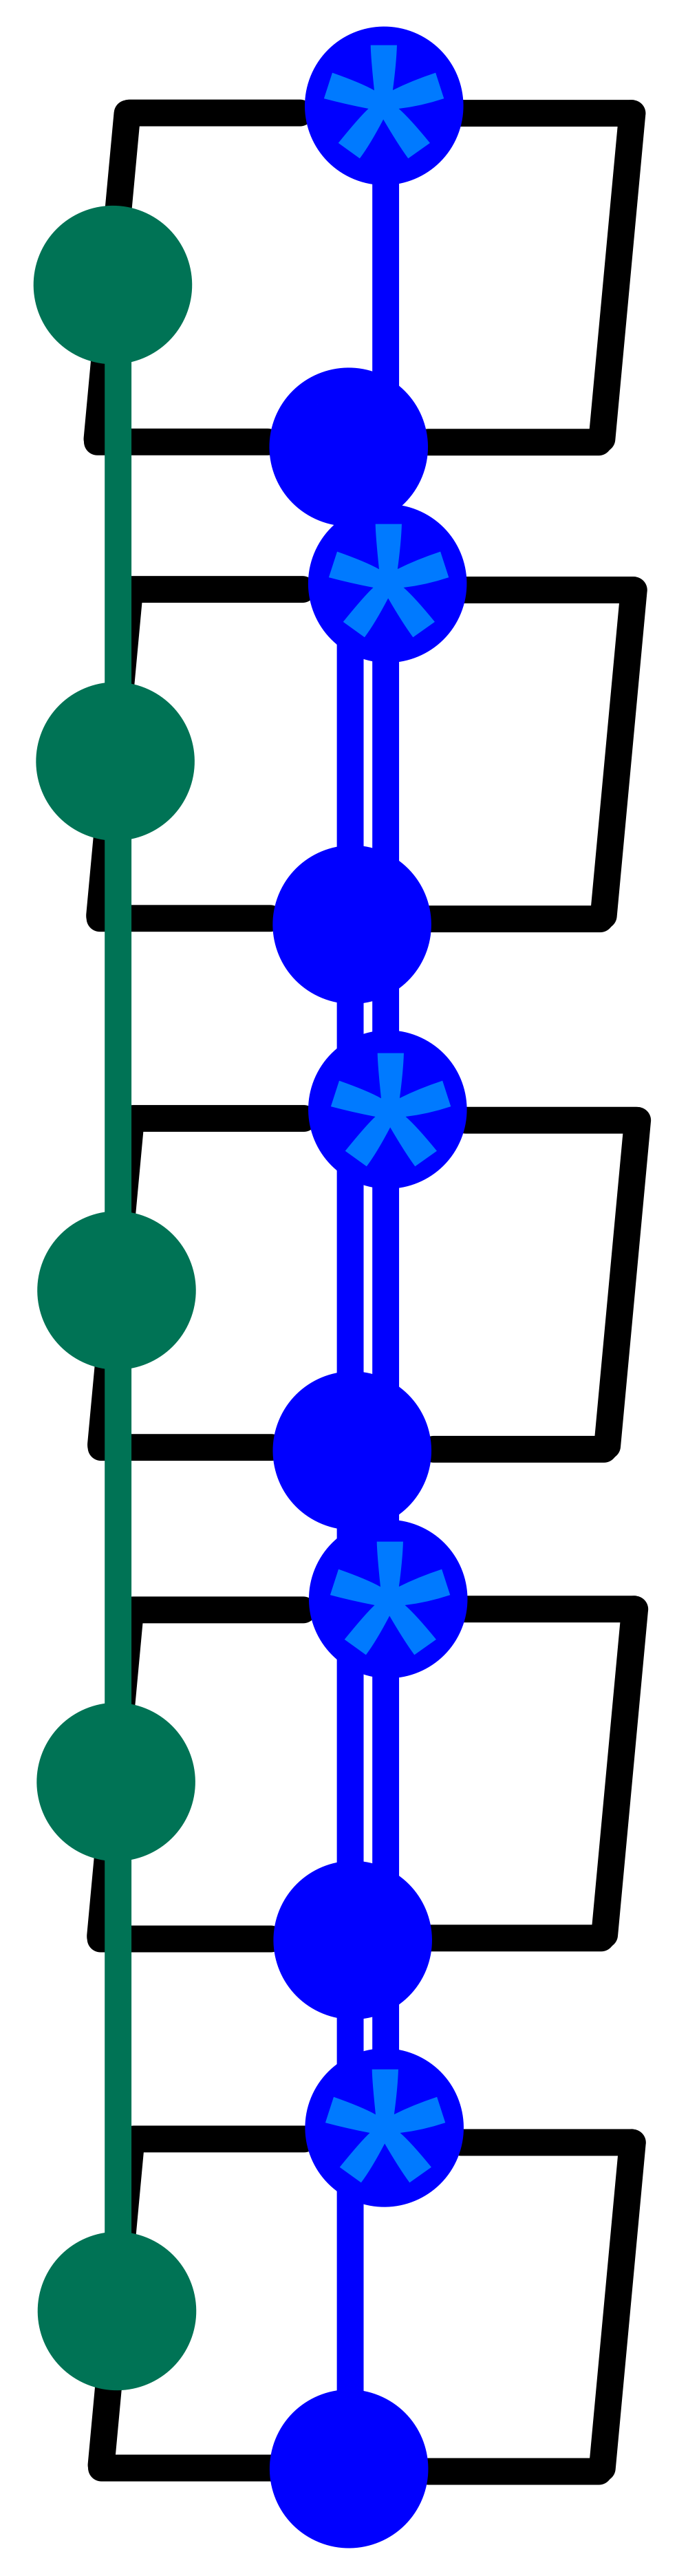
\includegraphics[height=4cm]{E_bc_l.png}} \\
	\left(
	\textcolor{ForestGreen}{L_h^{[n_x^c]}}
	\middle\vert
	\begin{array}{c}
	\textcolor{blue}{\overline{C}^{[n_x^c]}} \\
	\textcolor{blue}{C^{[n_x^c]}}
	\end{array}
	\middle\vert
	\mathbbm{1}
	\right)
	\end{array}
	+
	\begin{array}{c}
	\raisebox{-0.5\height}{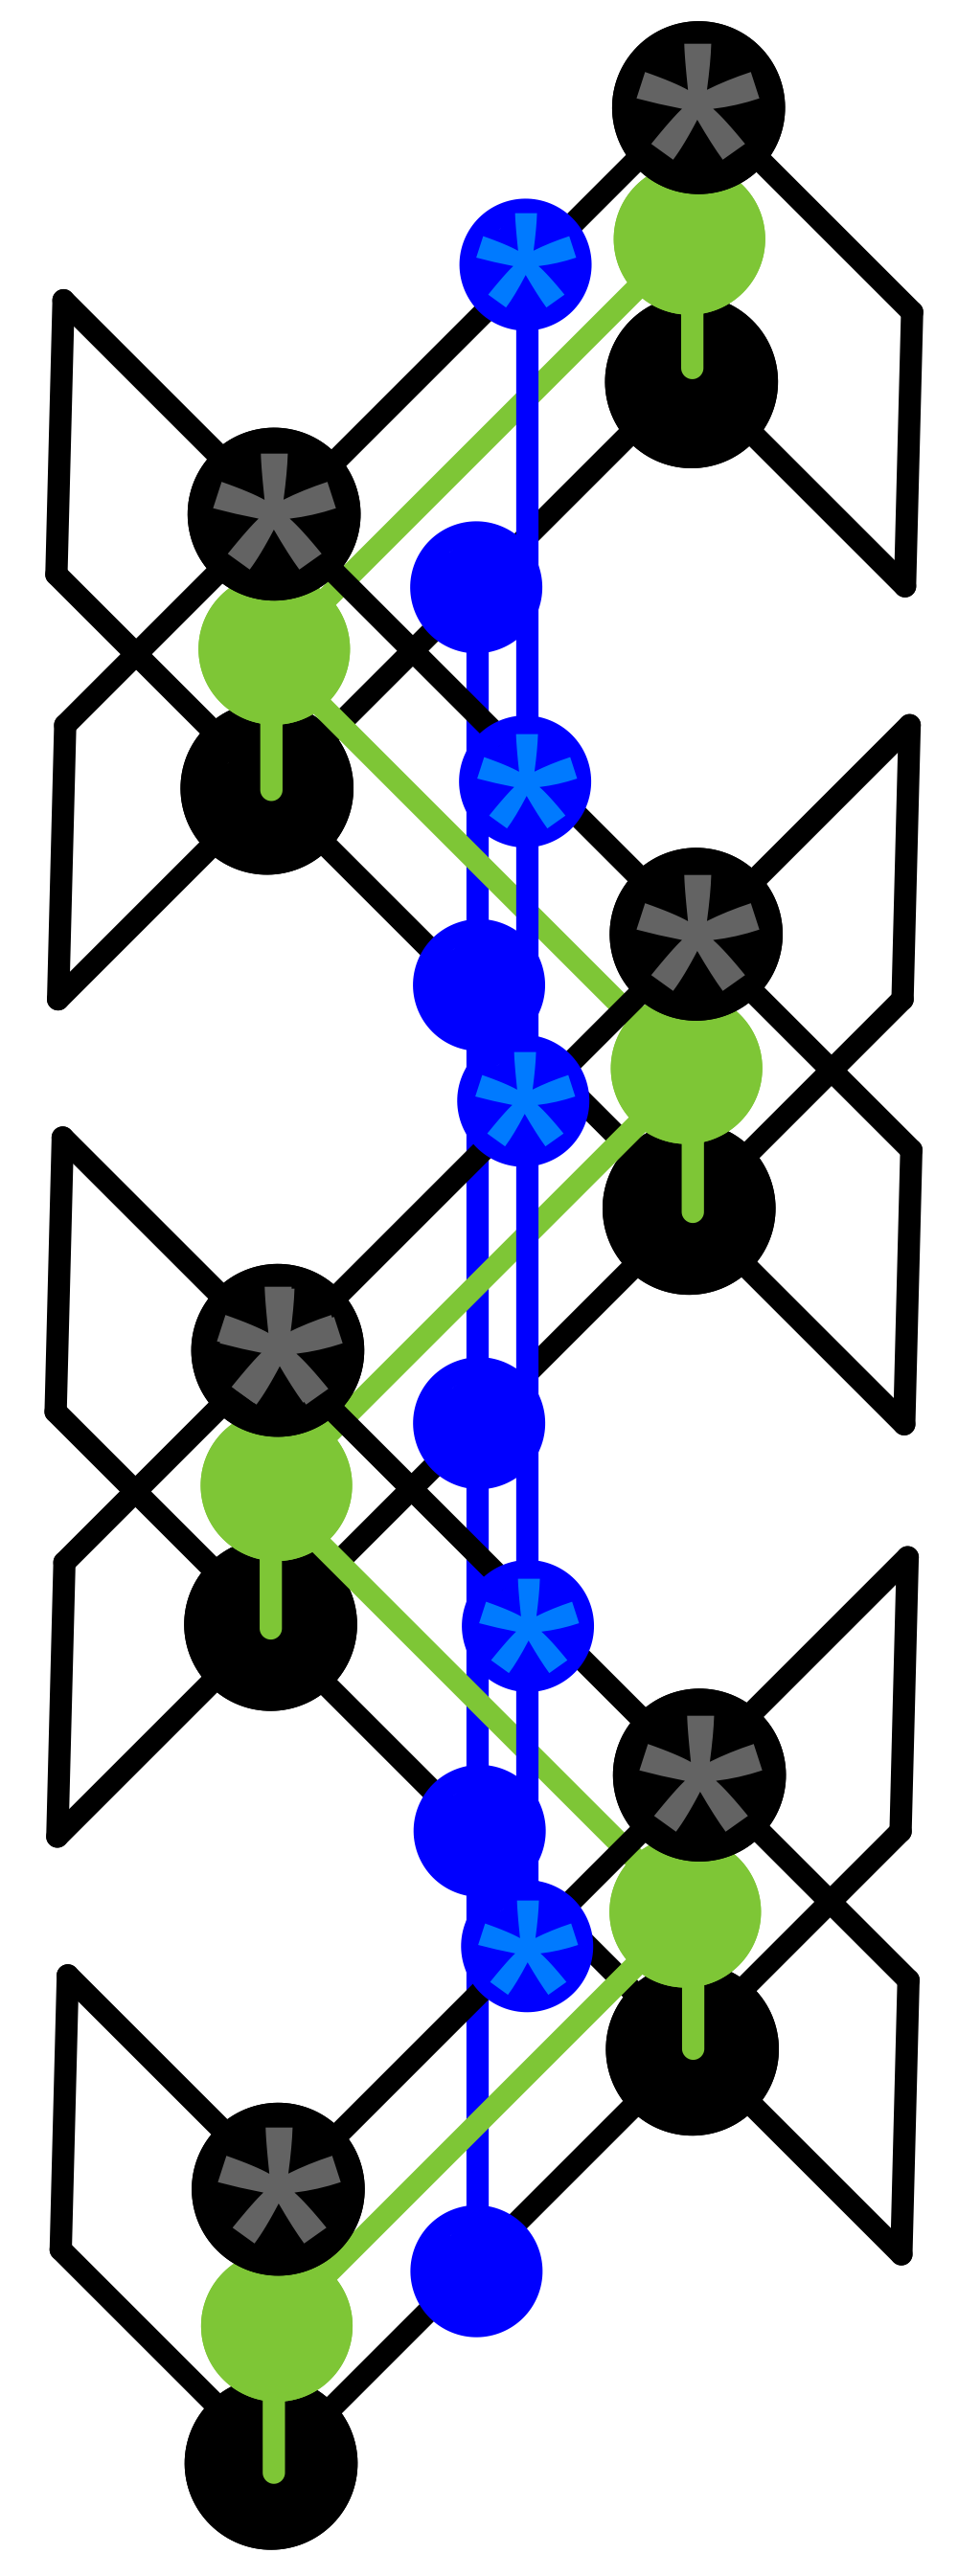
\includegraphics[height=5cm]{E_bc_c.png}} \\
	\left(
	\begin{array}{c}
	\overline{A}_L^{[n_x^c]} \\
	\textcolor{LimeGreen}{h_L^{[n_x^c, n_x^c +1]}} \\
	 A_L^{[n_x^c]}
	\end{array}
	\middle\vert
	\begin{array}{c}
	\textcolor{blue}{\overline{C}^{[n_x^c]}} \\
	\textcolor{blue}{C^{[n_x^c]}}
	\end{array}
	\middle\vert
	\begin{array}{c}
	\overline{A}_R^{[n_x^c+1]} \\
	\textcolor{LimeGreen}{h_R^{[n_x^c, n_x^c +1]}} \\
	 A_R^{[n_x^c+1]} 
	\end{array}
	\right)
	\end{array}
	+
	\begin{array}{c}
	\raisebox{-0.5\height}{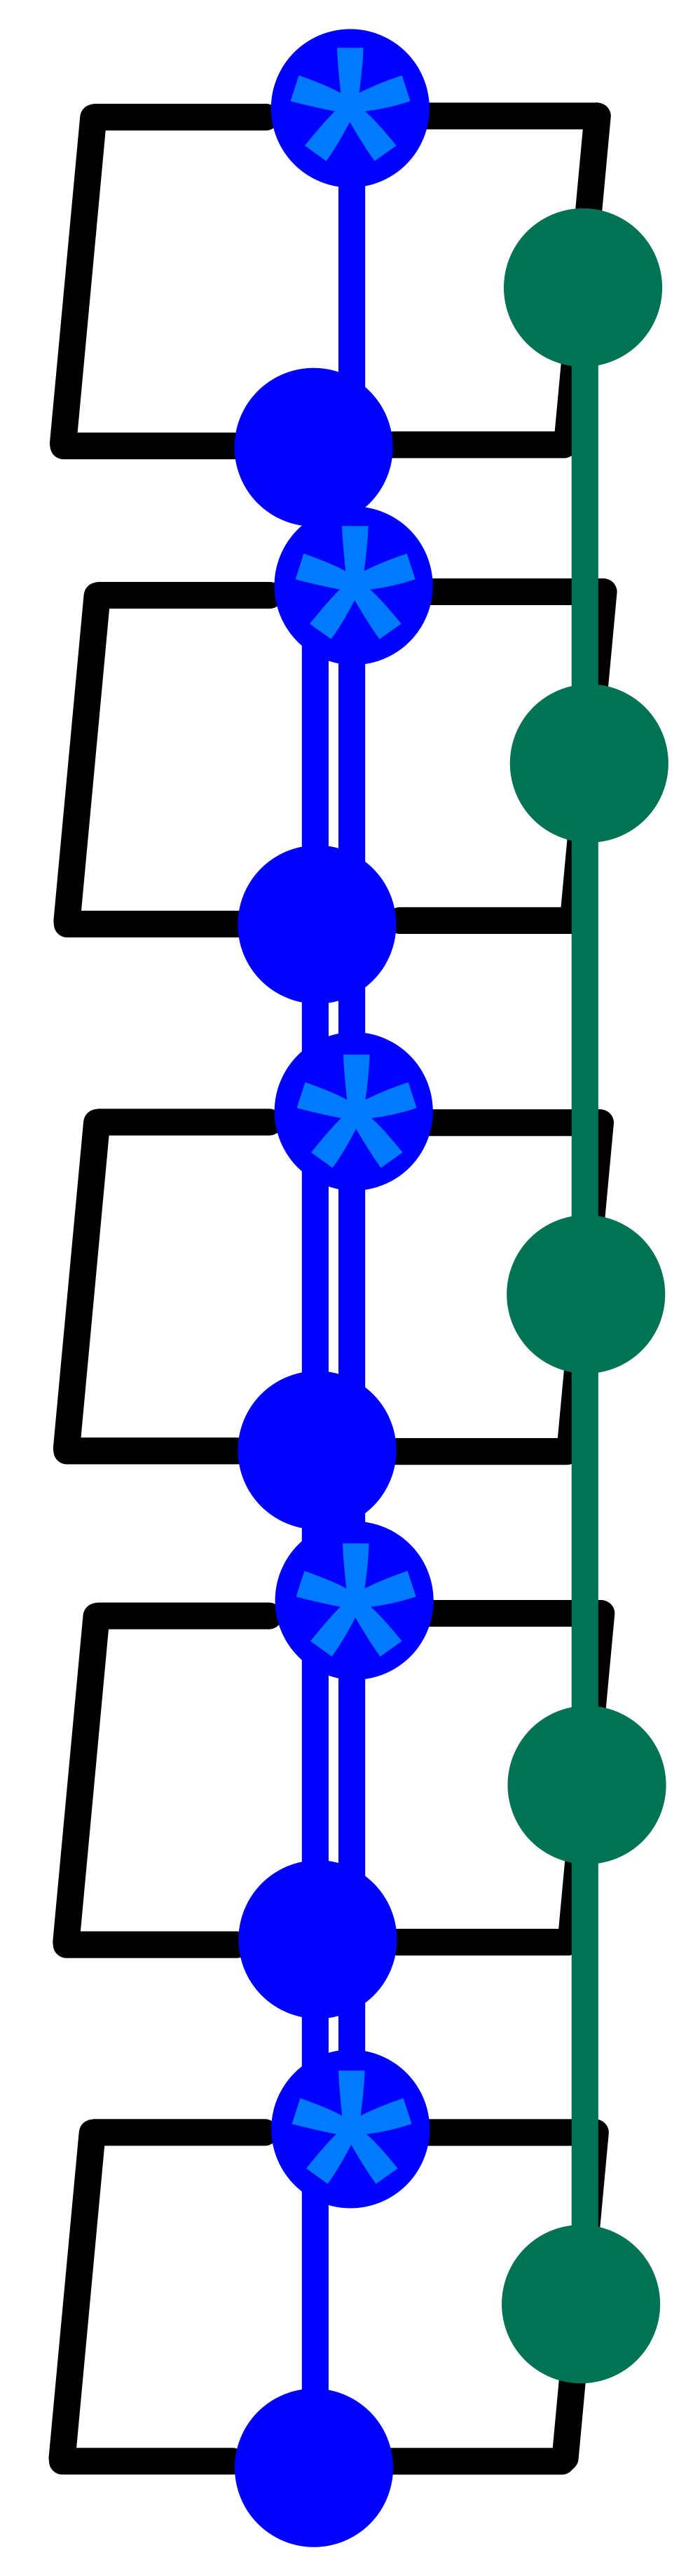
\includegraphics[height=4cm]{E_bc_r.png}} \\
	\left(
	\mathbbm{1}
	\middle\vert
	\begin{array}{c}
	\textcolor{blue}{\overline{C}^{[n_x^c]}} \\
	\textcolor{blue}{C^{[n_x^c]}}
	\end{array}
	\middle\vert
	\textcolor{ForestGreen}{R_h^{[n_x^c+1]}}
	\right)
	\end{array}
	\:.
\end{equation}

% boundary mps
\newpage
\noindent \underline{Boundary MPS} \\[0.5em]
\noindent We initialize $L_h^{[1]} = R_h^{[2L_x]} = 0$ and define the rest of the energy environments recursively as
\begin{align}
	\label{eq:Lh_bMPS}
	\begin{array}{c}
	\raisebox{-0.5\height}{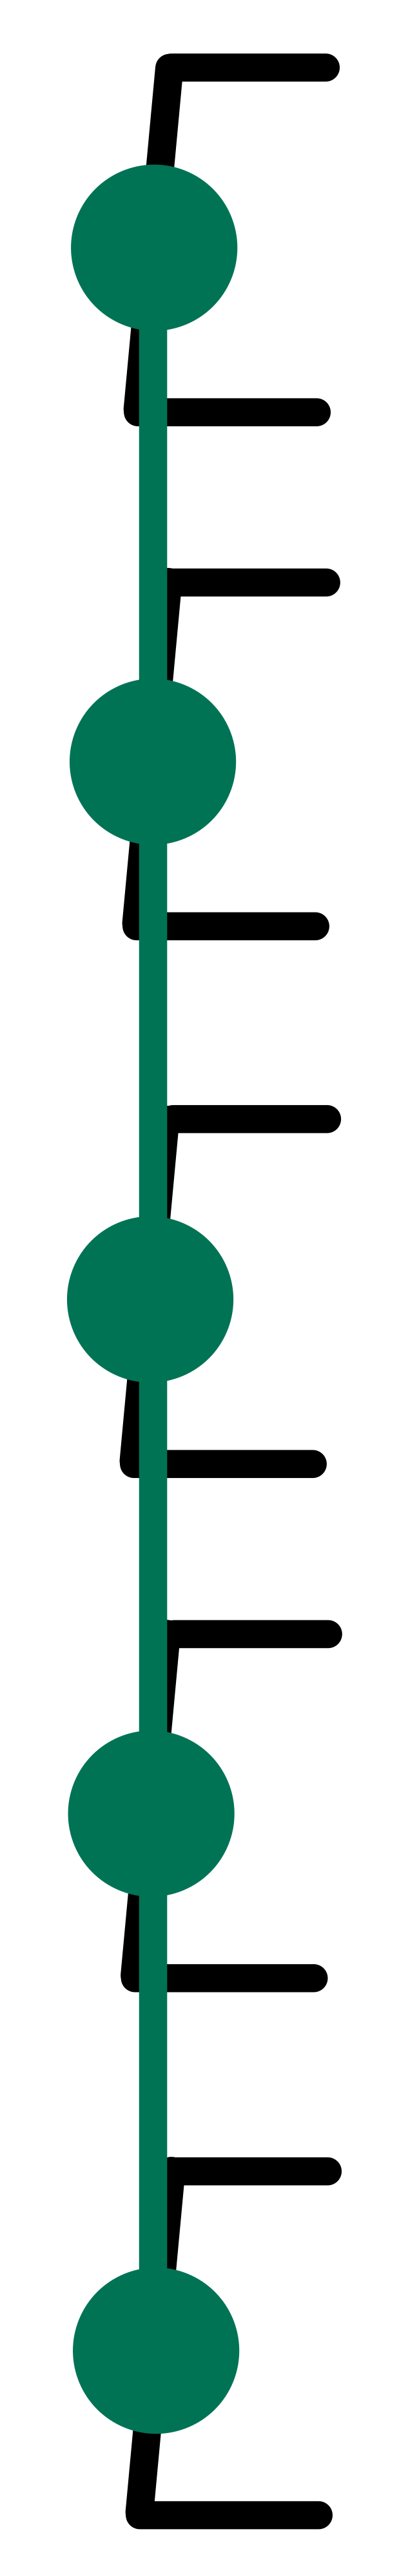
\includegraphics[height=3.6cm]{Lh.png}} \\
	\left( \textcolor{ForestGreen}{L_h^{[n_x]}} \right\vert
	\end{array}
	&=
	\begin{array}{c}
	\raisebox{-0.5\height}{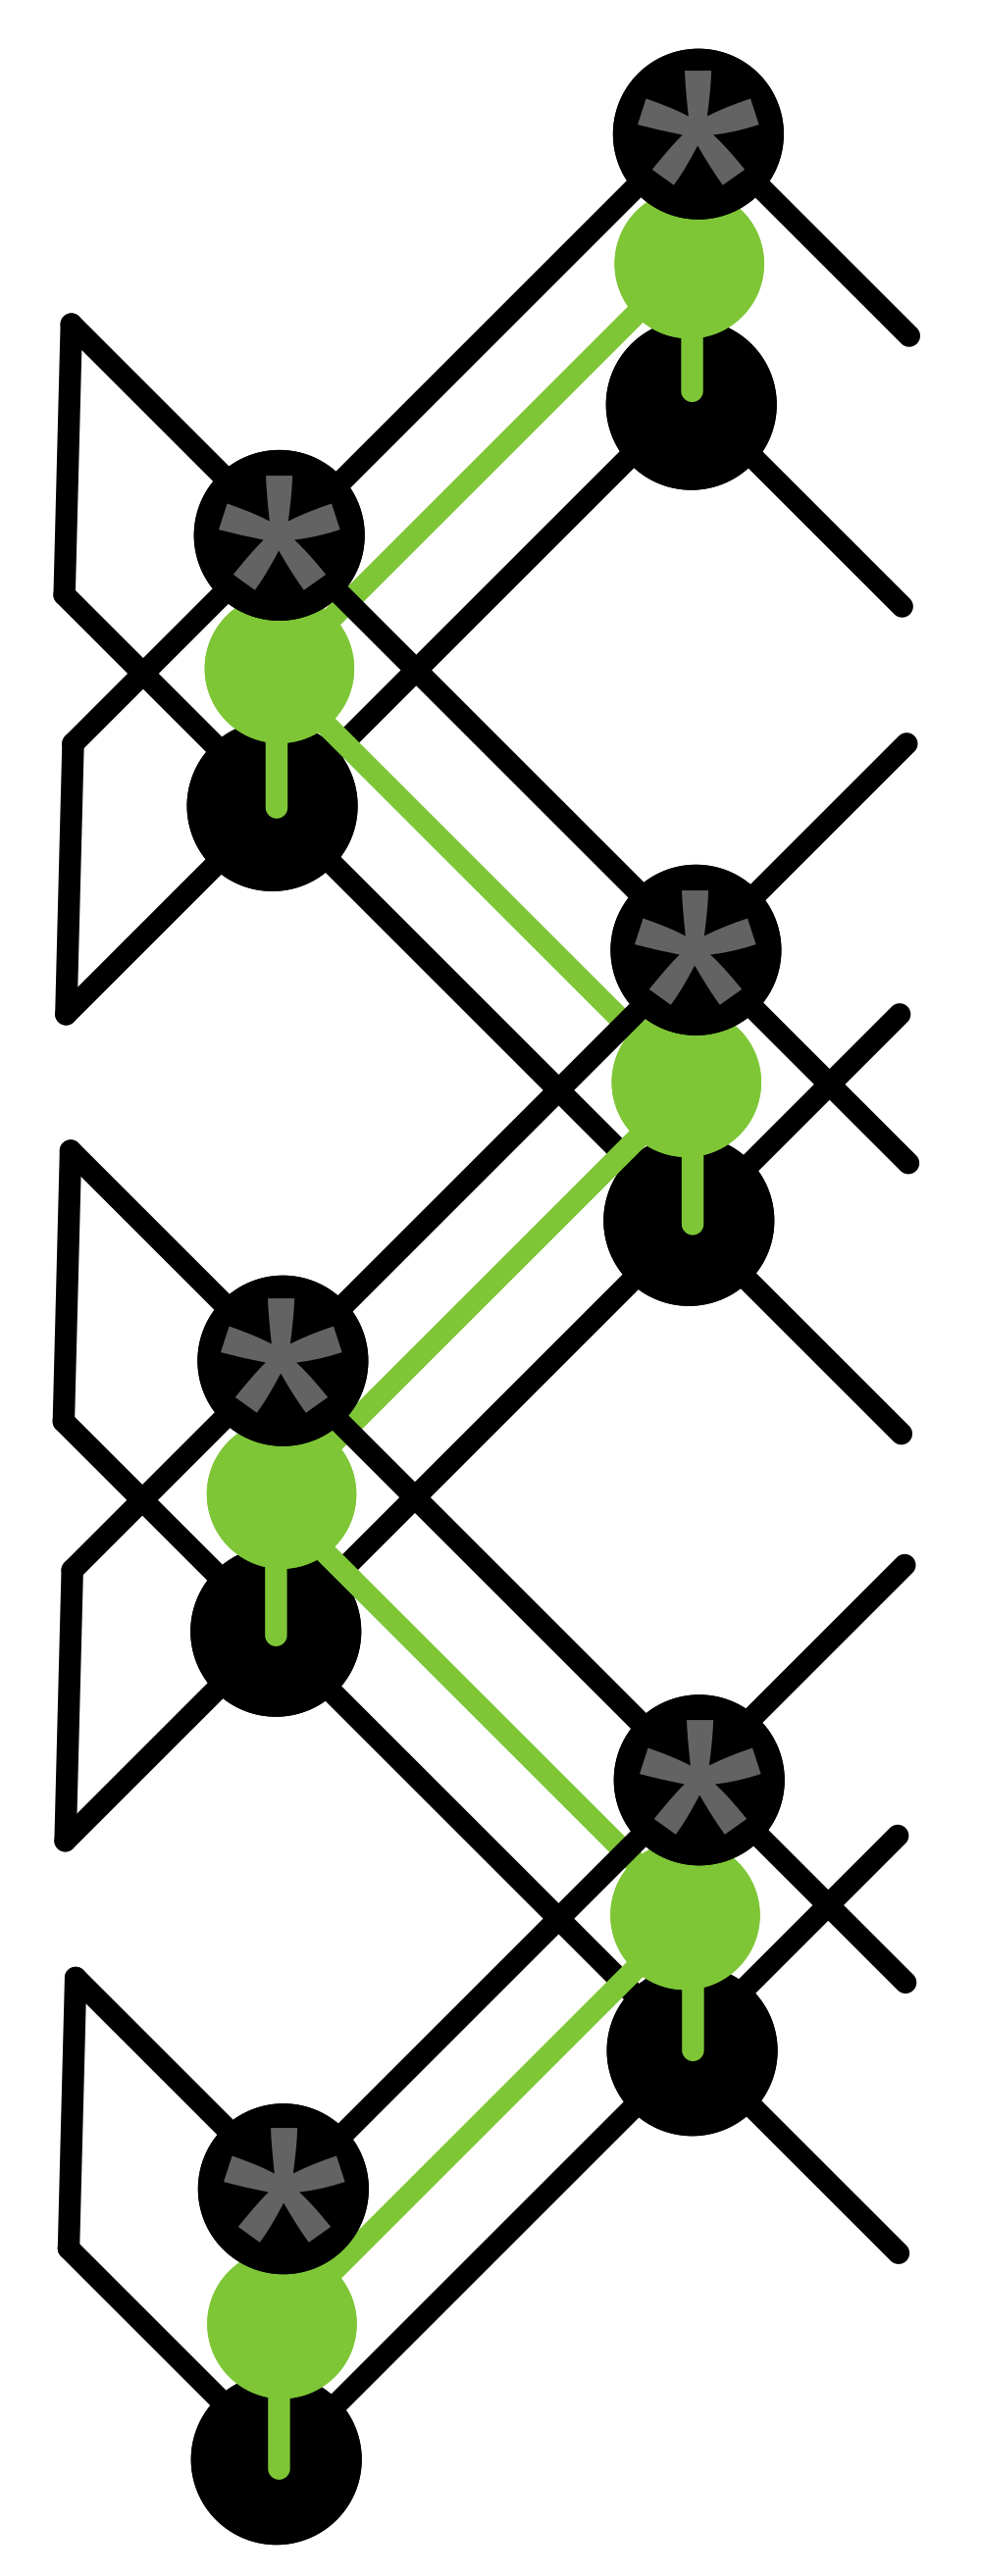
\includegraphics[height=4.5cm]{Lh1.png}} \\
	\left(
	\begin{array}{c}
	\overline{A}_L^{[n_x-1]} \overline{A}_L^{[n_x]} \\
	\textcolor{LimeGreen}{h^{[n_x-1, n_x]}} \\
	A_L^{[n_x-1]} A_L^{[n_x]}
	\end{array}
	\right\vert
	\end{array}
	+
	\begin{array}{c}
	\raisebox{-0.5\height}{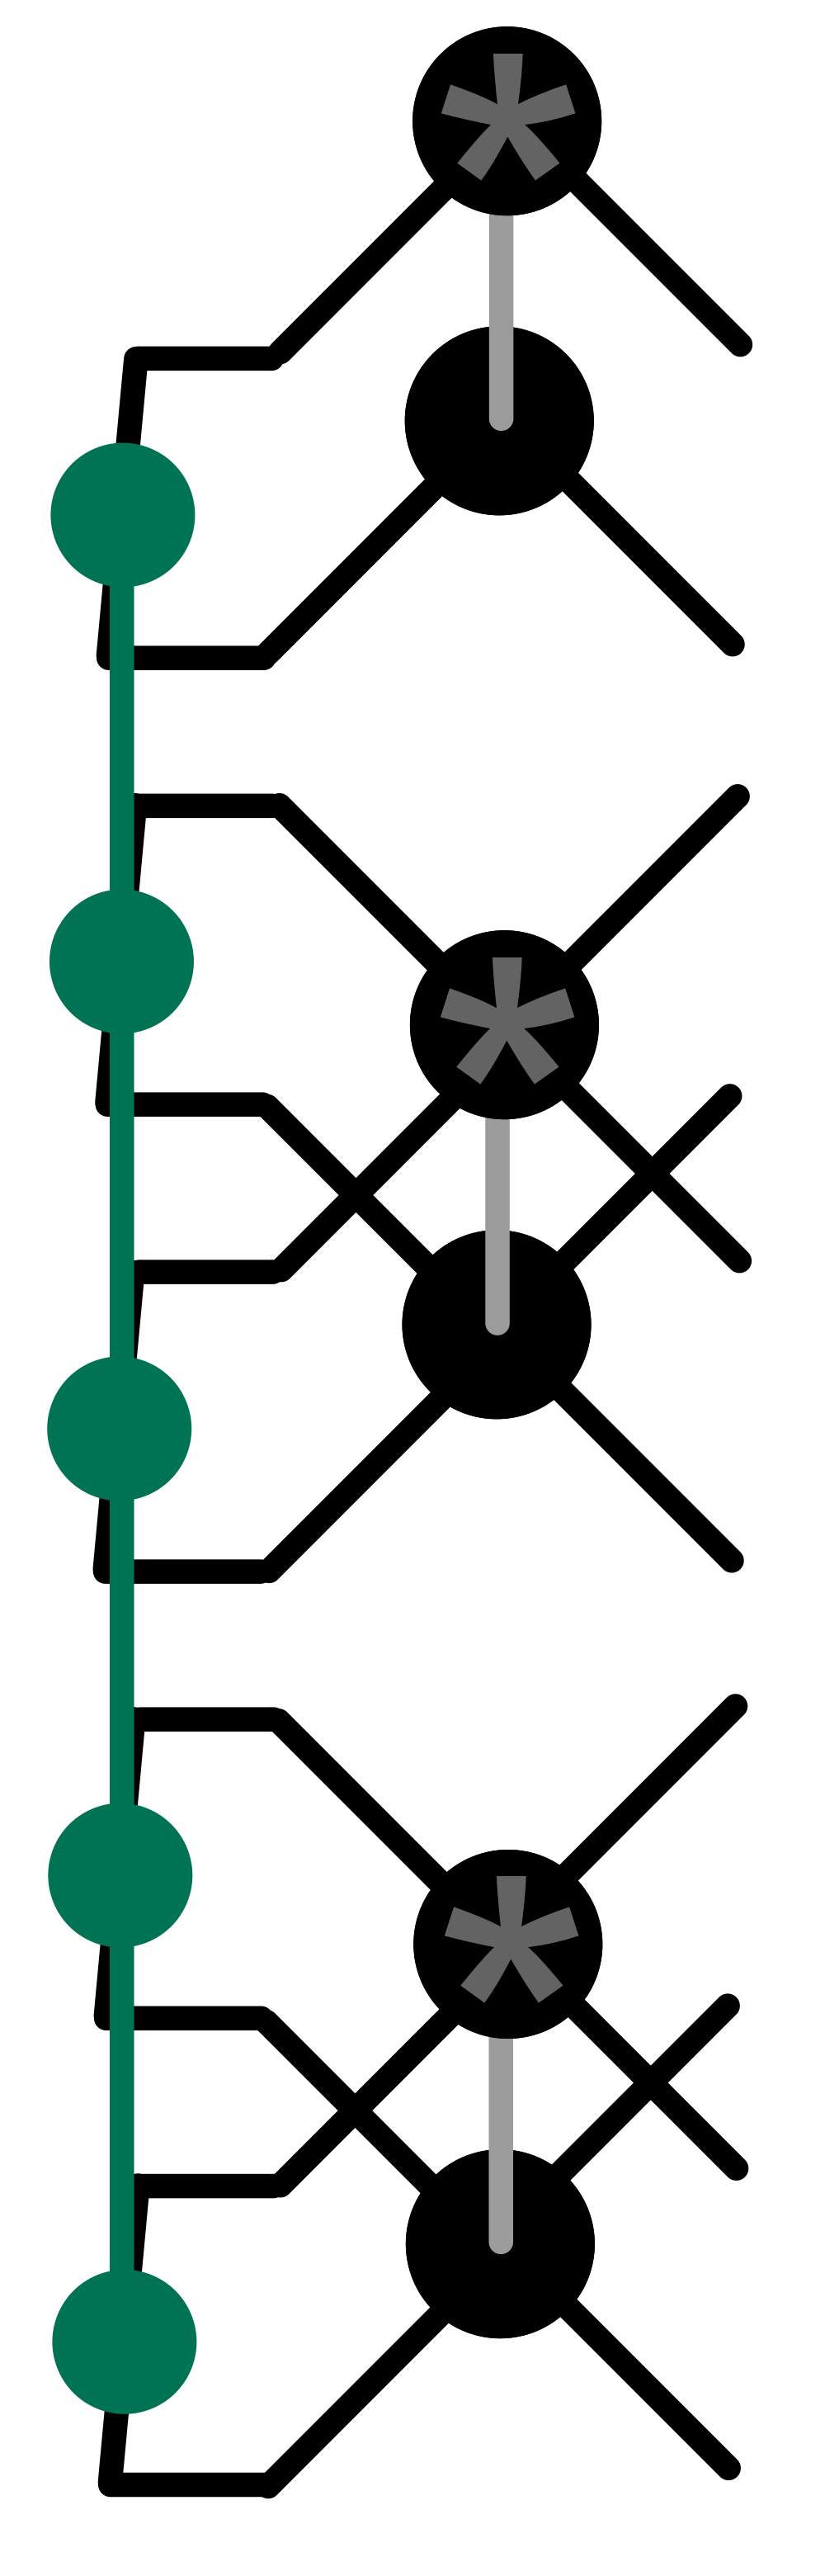
\includegraphics[height=4.2cm]{Lh2.png}} \\
	\left(
	\textcolor{ForestGreen}{L_h^{[n_x-1]}}
	\right\vert
	\begin{array}{c}
	\overline{A}_L^{[n_x]} \\
	A_L^{[n_x]}
	\end{array}
	\end{array}
	\textstyle (n_x = 2, \ldots, 2 L_x),
	\\
	\label{eq:Rh_bMPS}
	\begin{array}{c}
	\raisebox{-0.5\height}{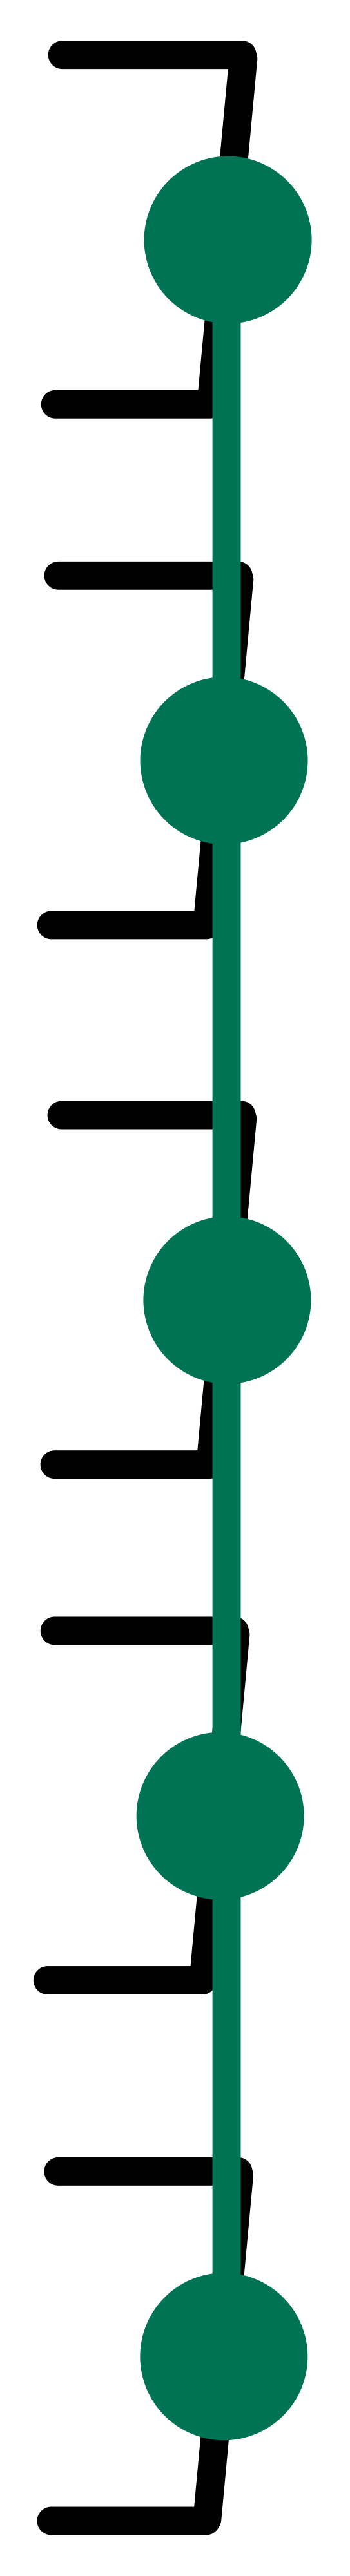
\includegraphics[height=3.6cm]{Rh.png}} \\
	\left\vert \textcolor{ForestGreen}{R_h^{[n_x]}} \right)
	\end{array}
	&=
	\begin{array}{c}
	\raisebox{-0.5\height}{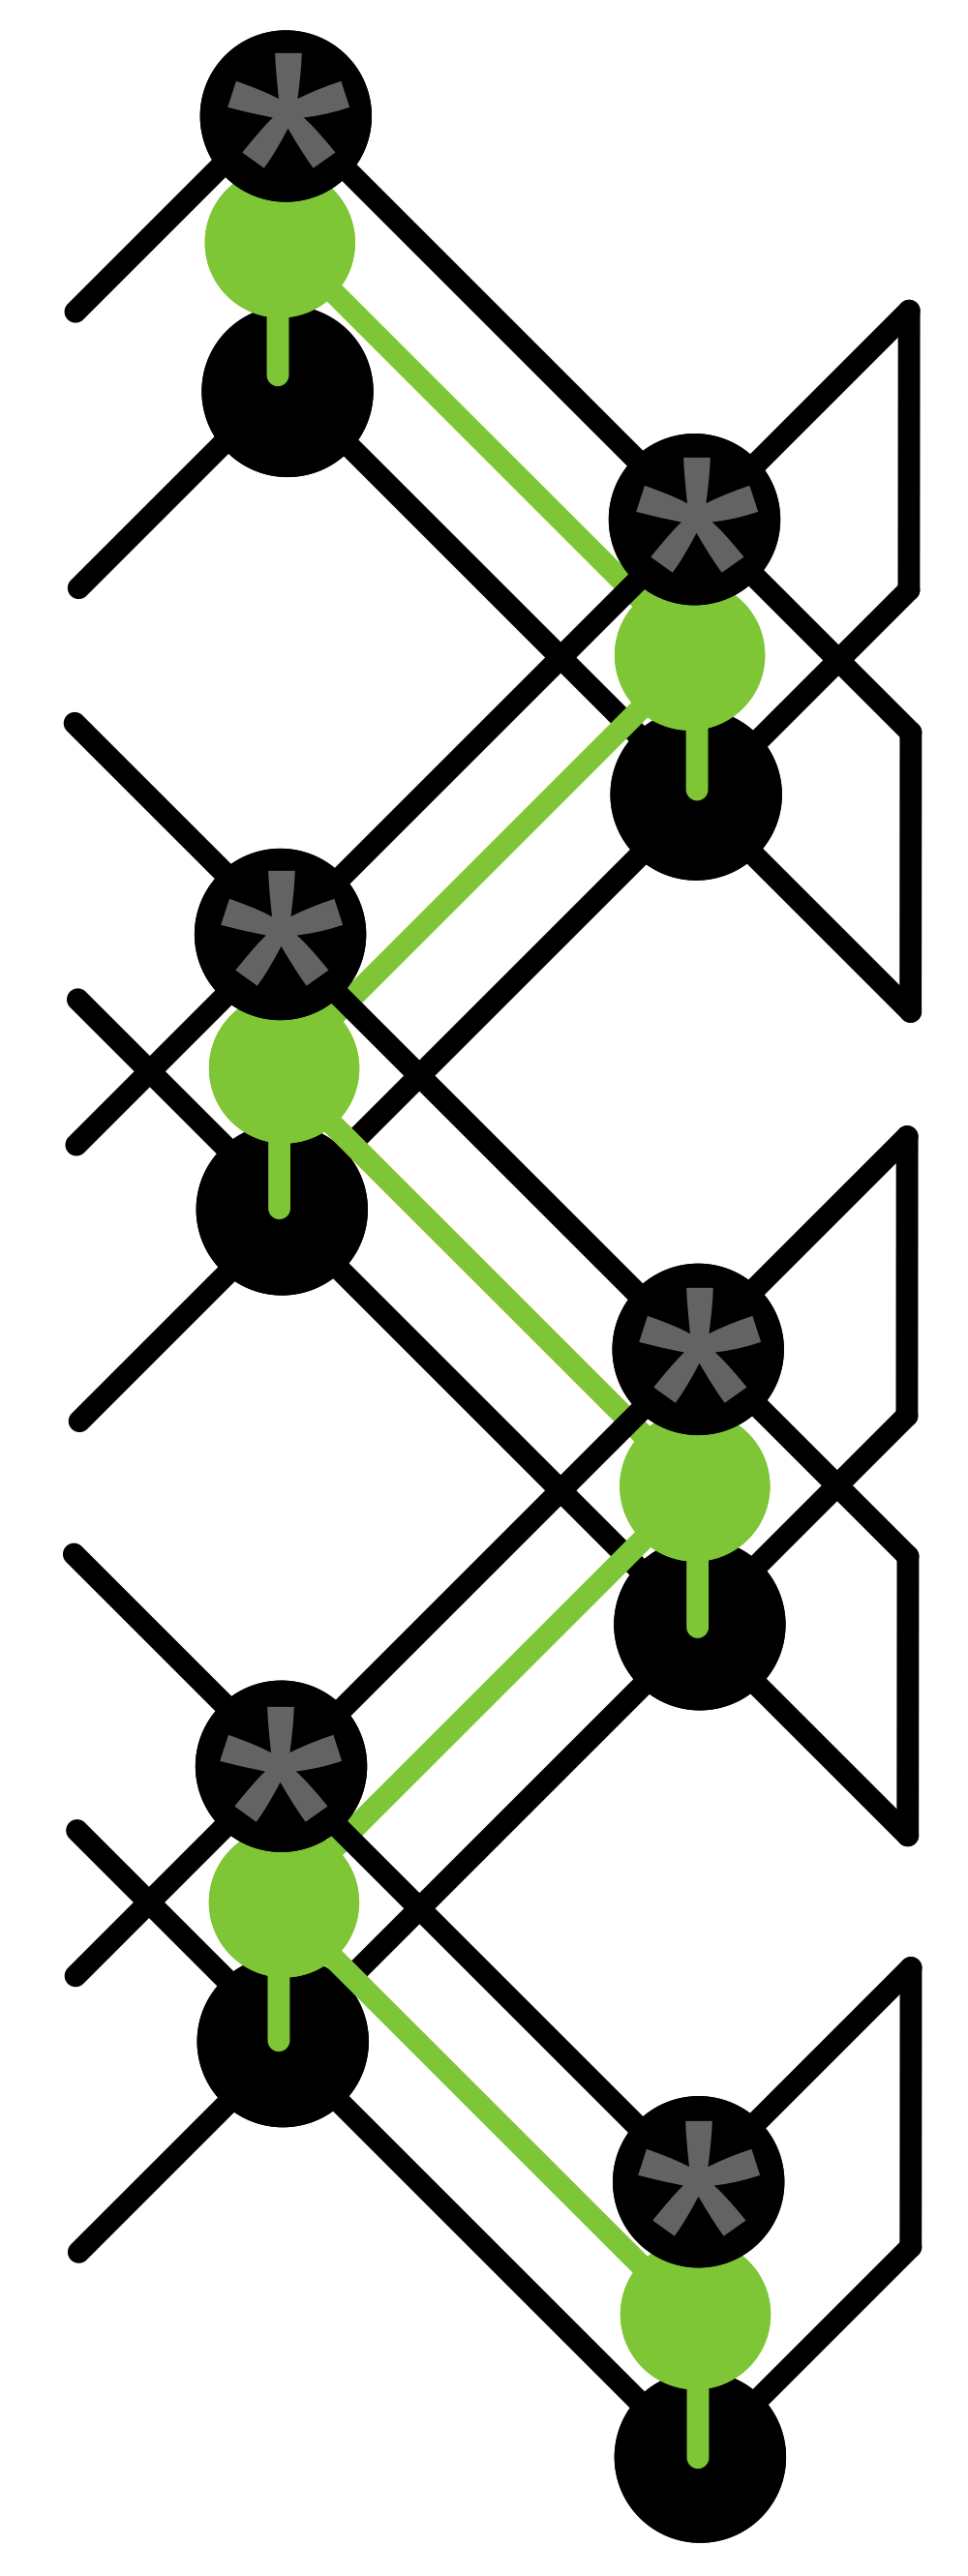
\includegraphics[height=4.5cm]{Rh1.png}} \\
	\left\vert
	\begin{array}{c}
	\overline{A}_R^{[n_x]} \overline{A}_R^{[n_x+1]} \\
	\textcolor{LimeGreen}{h^{[n_x, n_x+1]}} \\
	A_R^{[n_x]} A_R^{[n_x+1]}
	\end{array}
	\right)
	\end{array}
	+
	\begin{array}{c}
	\raisebox{-0.5\height}{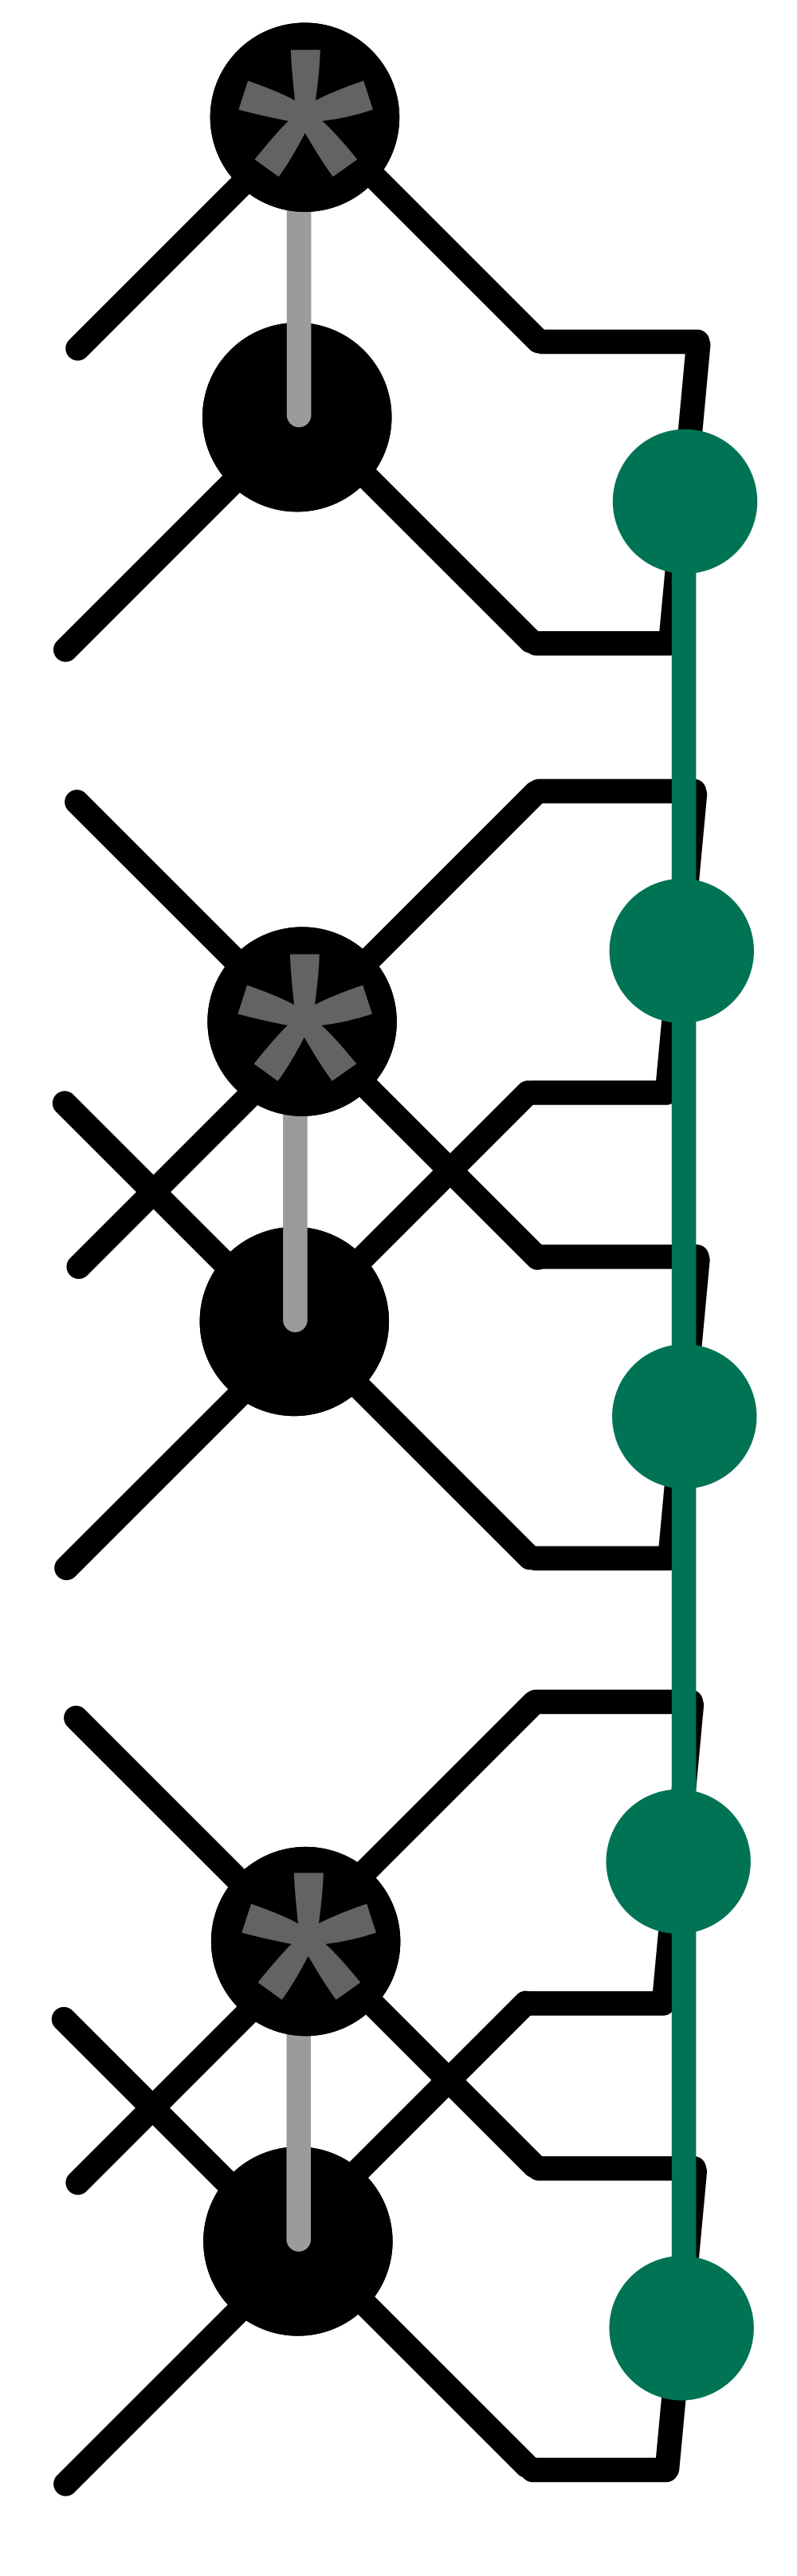
\includegraphics[height=4.2cm]{Rh2.png}} \\
	\begin{array}{c}
	\overline{A}_R^{[n_x]} \\
	A_R^{[n_x]}
	\end{array}
	\left\vert
	\textcolor{ForestGreen}{R_h^{[n_x+1]}}
	\right)
	\end{array}
	\textstyle (n_x = 2 L_x - 1, \ldots, 1).
\end{align}
Since up to a horizontal $\text{left} \leftrightarrow \text{right}$ flip of the $A_R$-tensors, $R_h^{[n_x]}$ has the same structure as $L_h^{[n_x]}$, it is enough to concentrate on the latter from now on. In the same way, after a vertical $\text{down} \leftrightarrow \text{up}$ flip of all involved tensors, $L_h^{[n_x]}$ for odd $n_x$ is in identical form to $L_h^{[n_x]}$ for even $n_x$ (the version drawn above):
\begin{equation}
	\raisebox{-0.5\height}{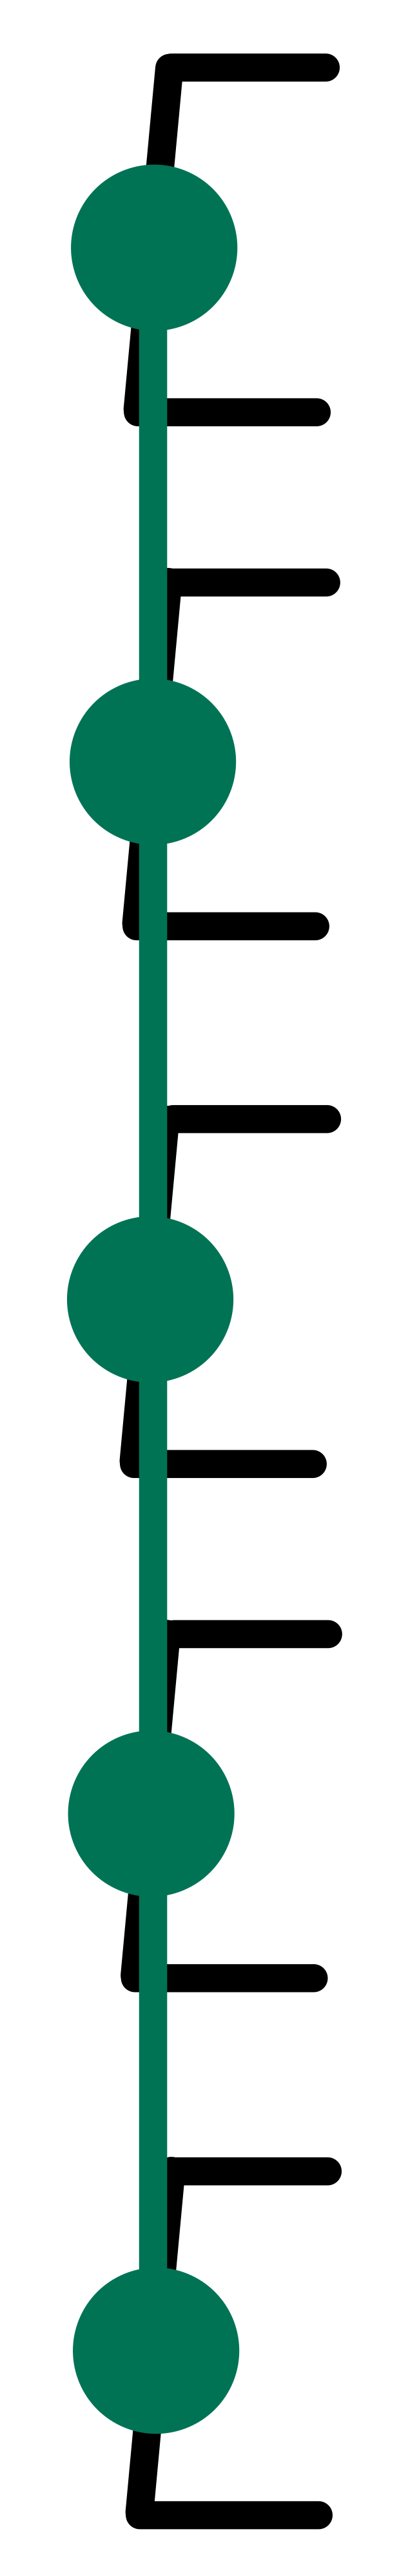
\includegraphics[height=3.6cm]{Lh.png}}
	\hspace{1em}=\hspace{1em}
	\raisebox{-0.5\height}{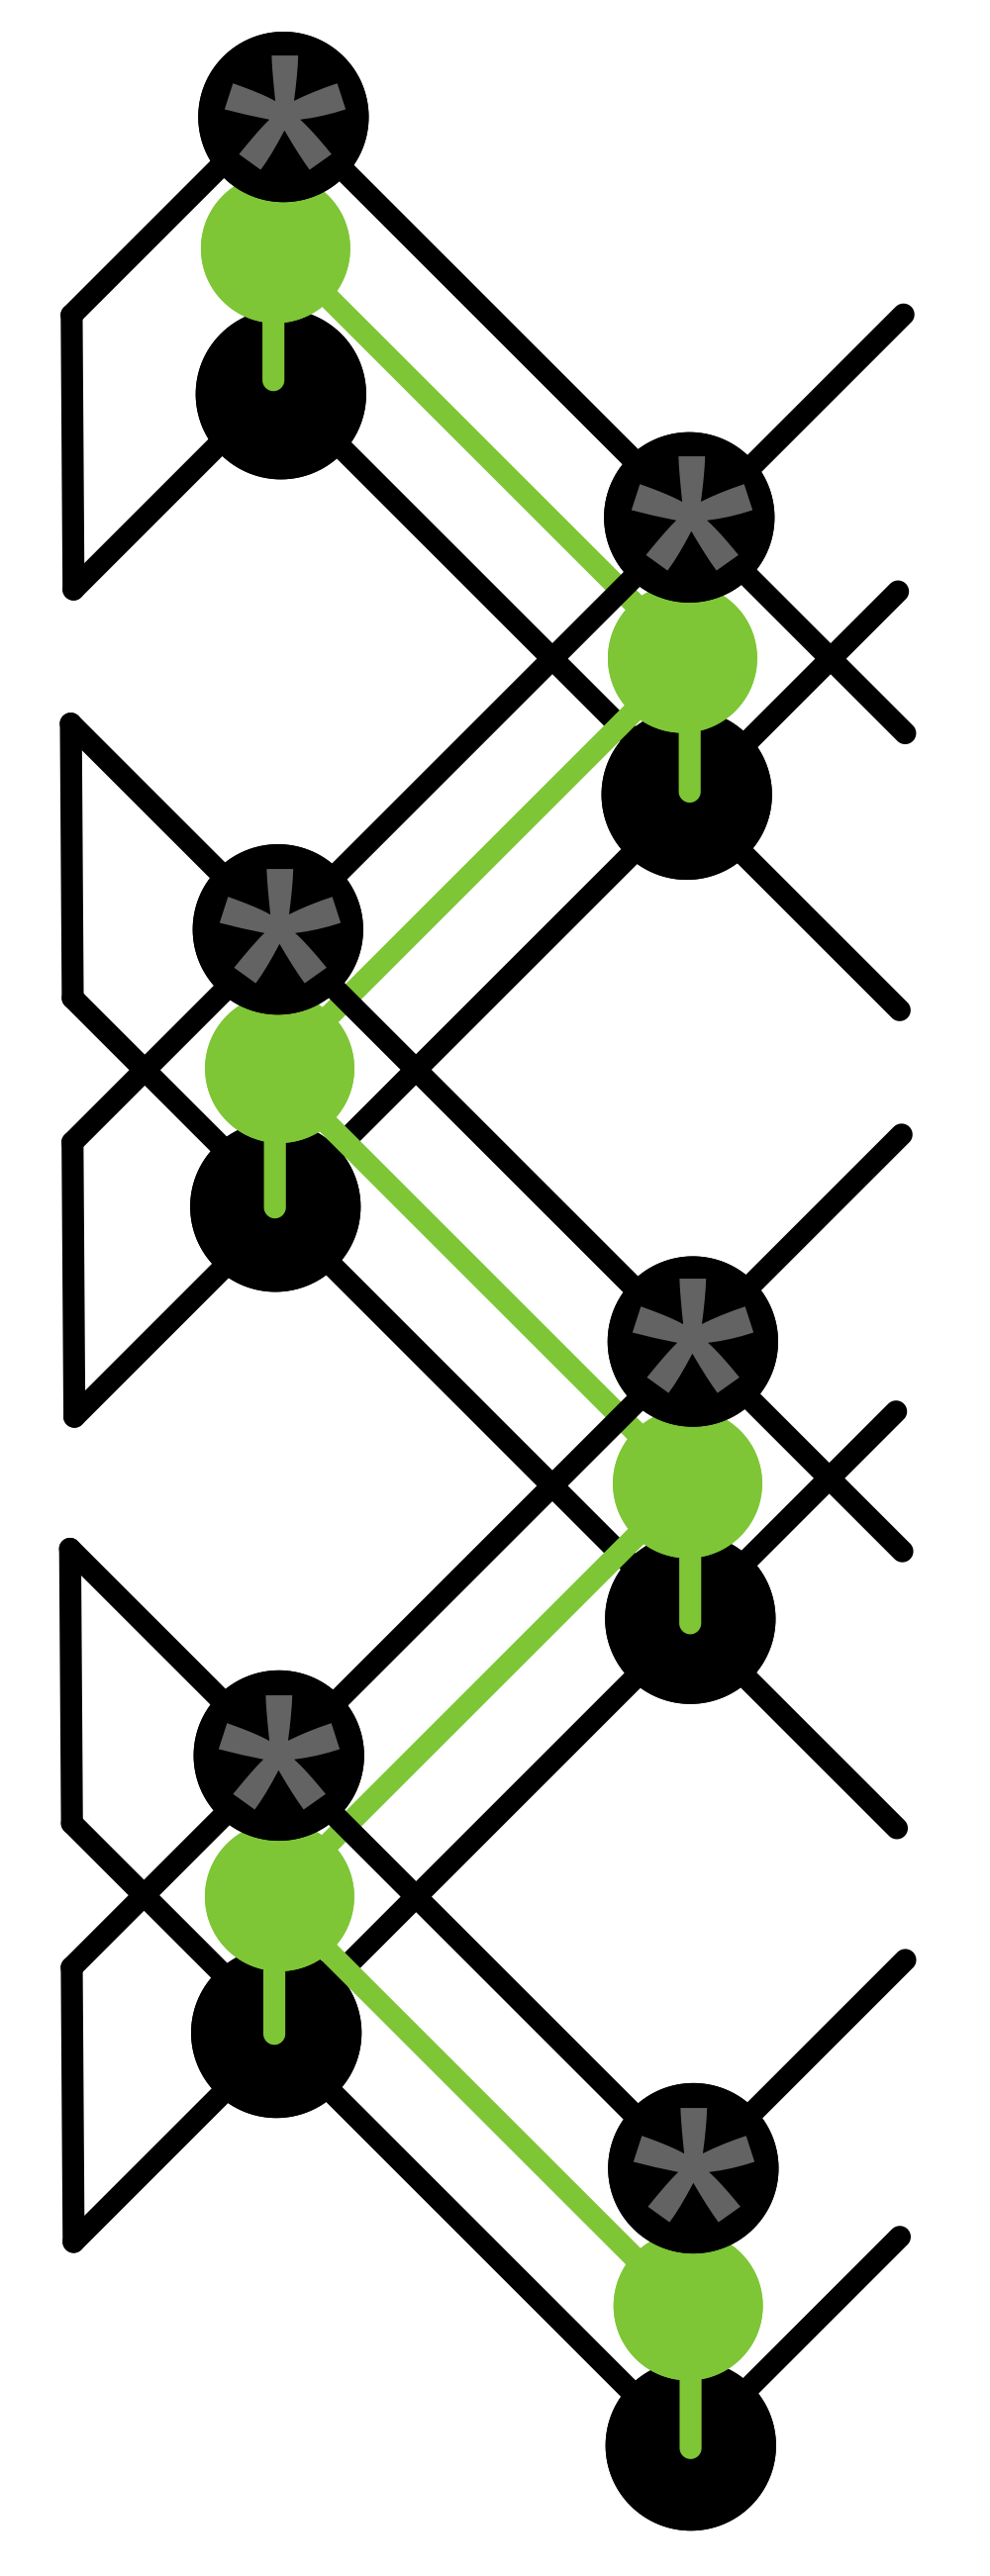
\includegraphics[height=4.5cm]{Lh1_odd.png}}
	\hspace{1em}+\hspace{1em}
	\raisebox{-0.5\height}{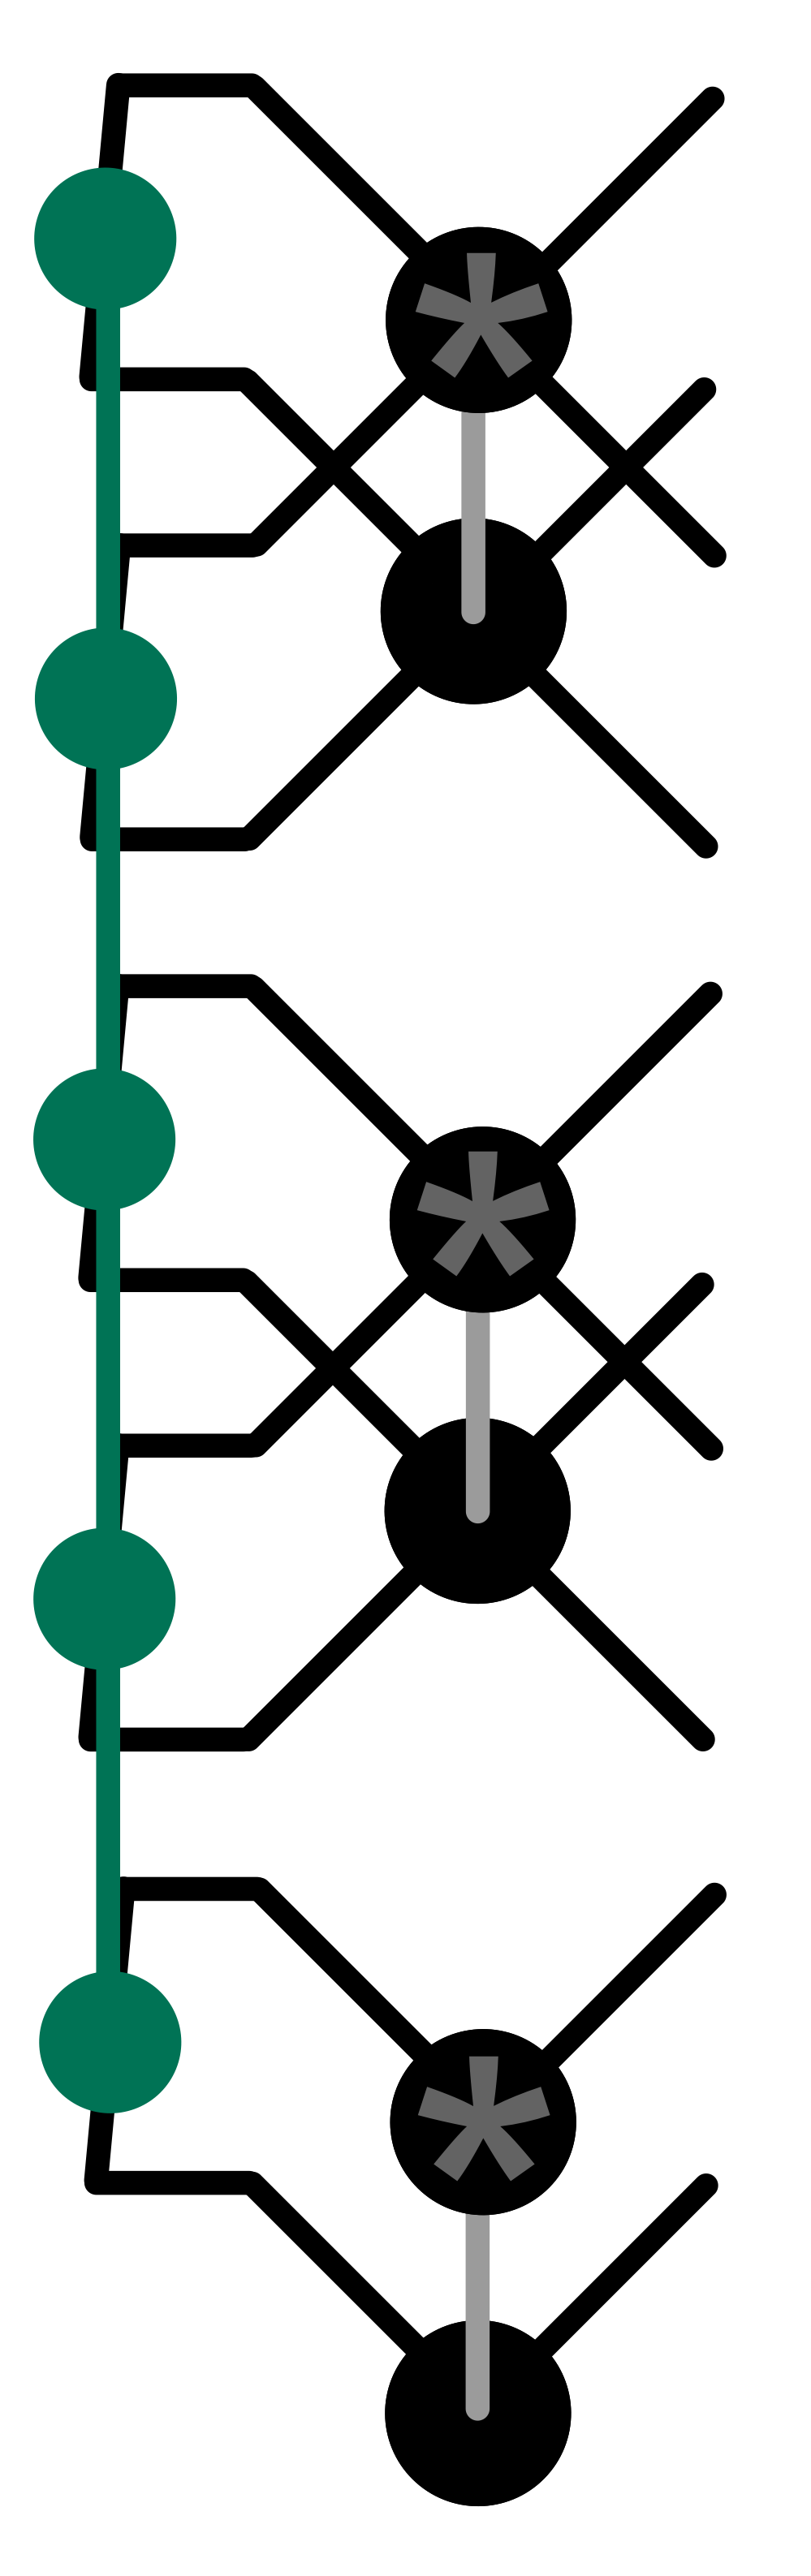
\includegraphics[height=4.2cm]{Lh2_odd.png}}
	\hspace{1em} \textstyle (n_x \text{ odd}).
\end{equation}
Interpreting the open ket and bra lattice legs as a double "physical" leg, we can treat $L_h^{[n_x]}$ as a \textit{boundary MPS} (bMPS). \\[0.5em]

\noindent In principle, we can compute $L_h^{[n_x]}$ exactly by allowing a maximal bMPS bond dimension of
\begin{equation}
	\chi_{\text{max}, b}^{\text{exact}} = D_{\text{max}}^{2(L_y-1)}.
\end{equation}
Due to the exponential growth of $\chi_{\text{max}, b}^{\text{exact}}$ with $L_y$ (e.g. $\chi_{\text{max}, b}^{\text{exact}} = 1,048,576$ for $L_y = 6$ and $D_{\text{max}} = 4$), the exact contraction becomes infeasible in practice. As a consequence, we need a method that efficiently compresses $L_h^{[n_x]}$ to a moderate bond dimension $\chi_{\text{max}, b}$, without loosing too much information about the effective Hamiltonian. For the $\text{DMRG}^2$ algorithm in section \ref{sec:dmrg2}, we take
\begin{equation}
	\chi_{\text{max}, b} = 6 D_{\text{max}}^{2}.
\end{equation}

\vspace*{2em}

% variational bc
\noindent \underline{Variational boundary compression} \\[0.5em]
The standard procedure for compressing a bMPS is variational optimization \cite{orus2014practical}. For $(L_h\vert$ in \eqref{eq:Lh_bMPS}, we denote the first term (that newly applies $h$ to the identity boundary) as $(L_h^{\text{new}}\vert$, and the second term (that transfers the boundary of all $h$s that already have been applied) as  $(L_h^{\text{transfer}}\vert$. With this we can formulate one local update of $\theta_2^{[n_y, n_y+1]}$, a two-site tensor of $(L_h\vert$, as the minimization problem
\begin{equation}
	\argmin_{\theta_2^{[n_y, n_y+1]}} 
	\left\Vert (L_h(\theta_2)\vert - (L_h^{\text{new}}\vert - (L_h^{\text{transfer}}\vert  \right\Vert^2_2.
\end{equation}
Taking the derivative of the norm cost function with respect to $\overline{\theta}_2$ gives the solution
\begin{equation} \label{eq:bc_update_theta2}
	\theta_2^{[n_y, n_y+1]}
	=
	\begin{array}{c}
	\raisebox{-0.5\height}{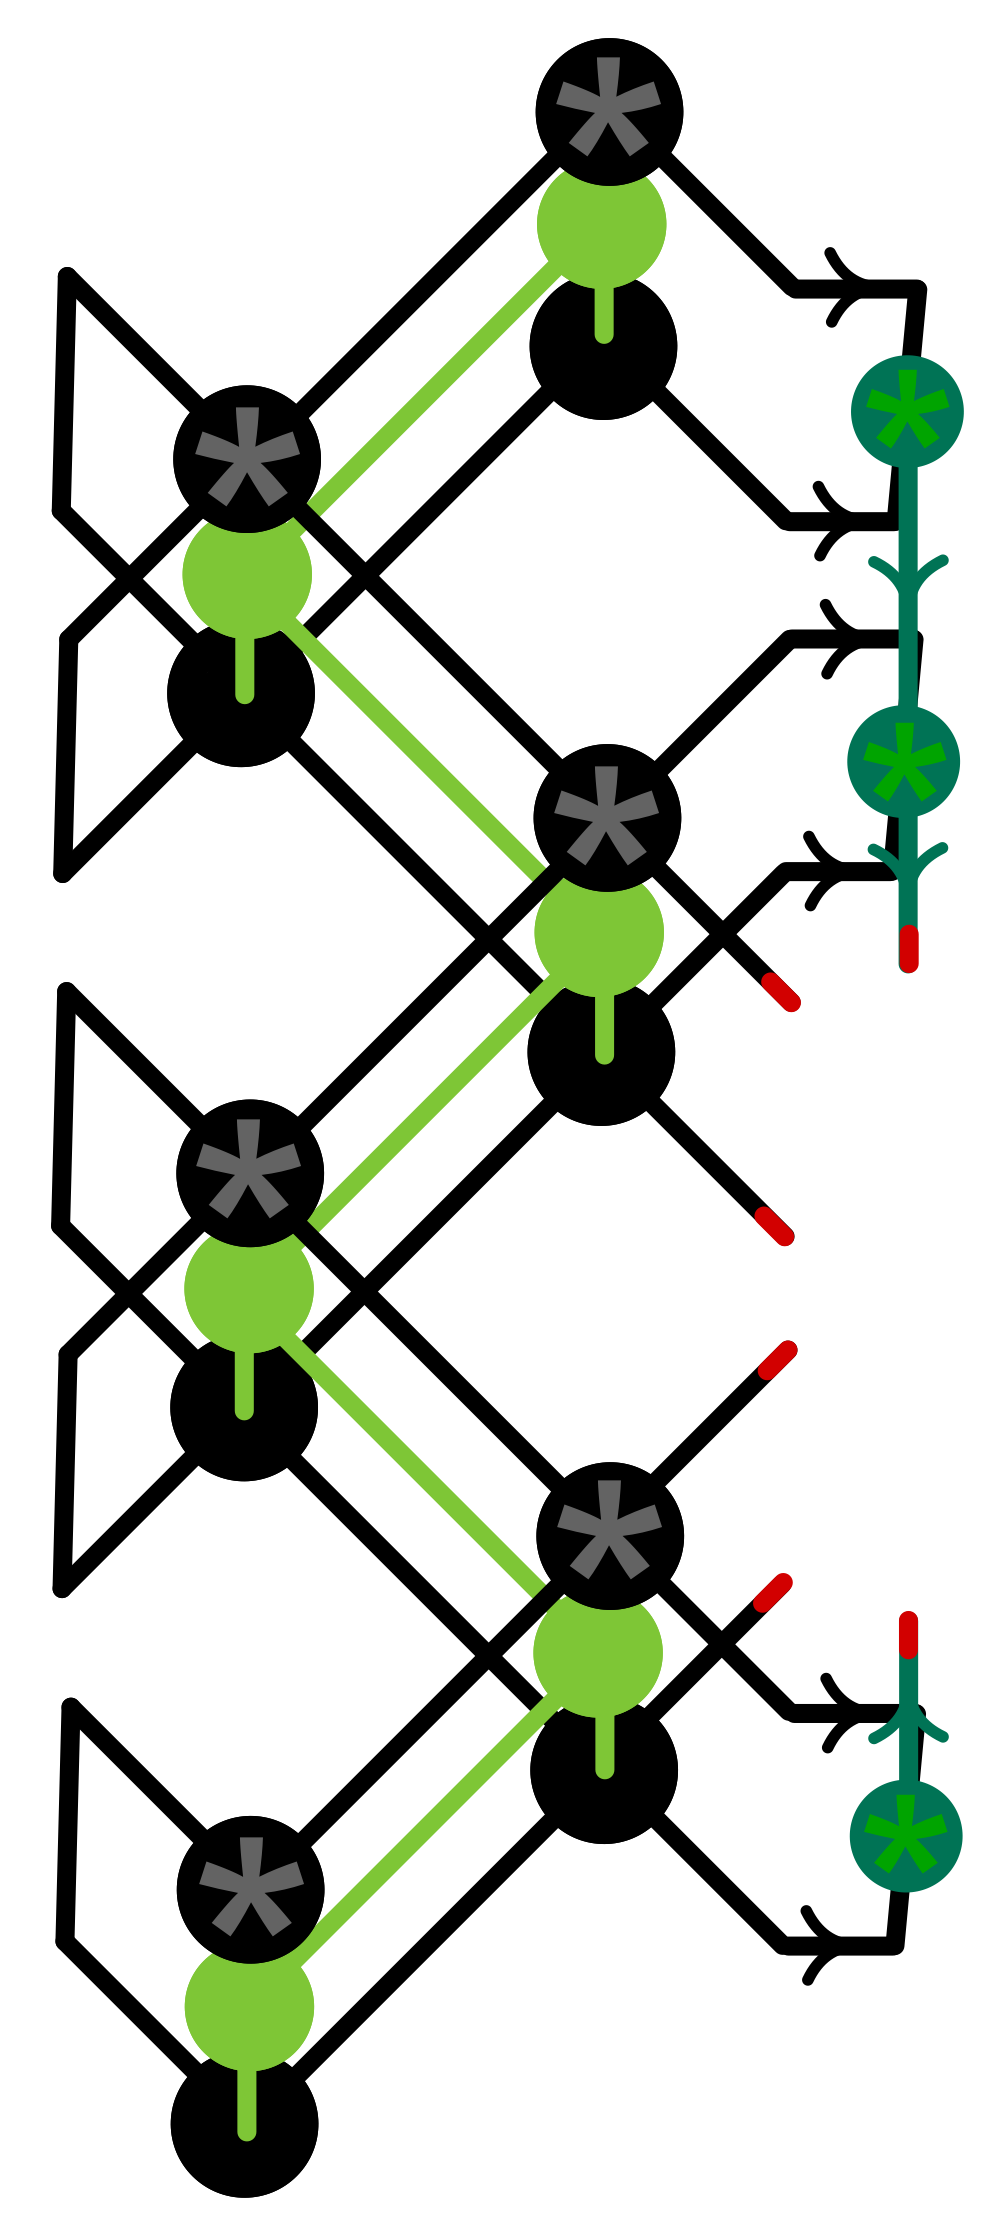
\includegraphics[height=4.5cm]{bc_theta_new.png}} \\
	\textstyle
	\left( L_h^{\text{new}} \middle\vert \partial_{\overline{\theta}_2} L_h(\overline{\theta}_2) \right)
	\end{array}
	+ 
	\begin{array}{c}
	\raisebox{-0.5\height}{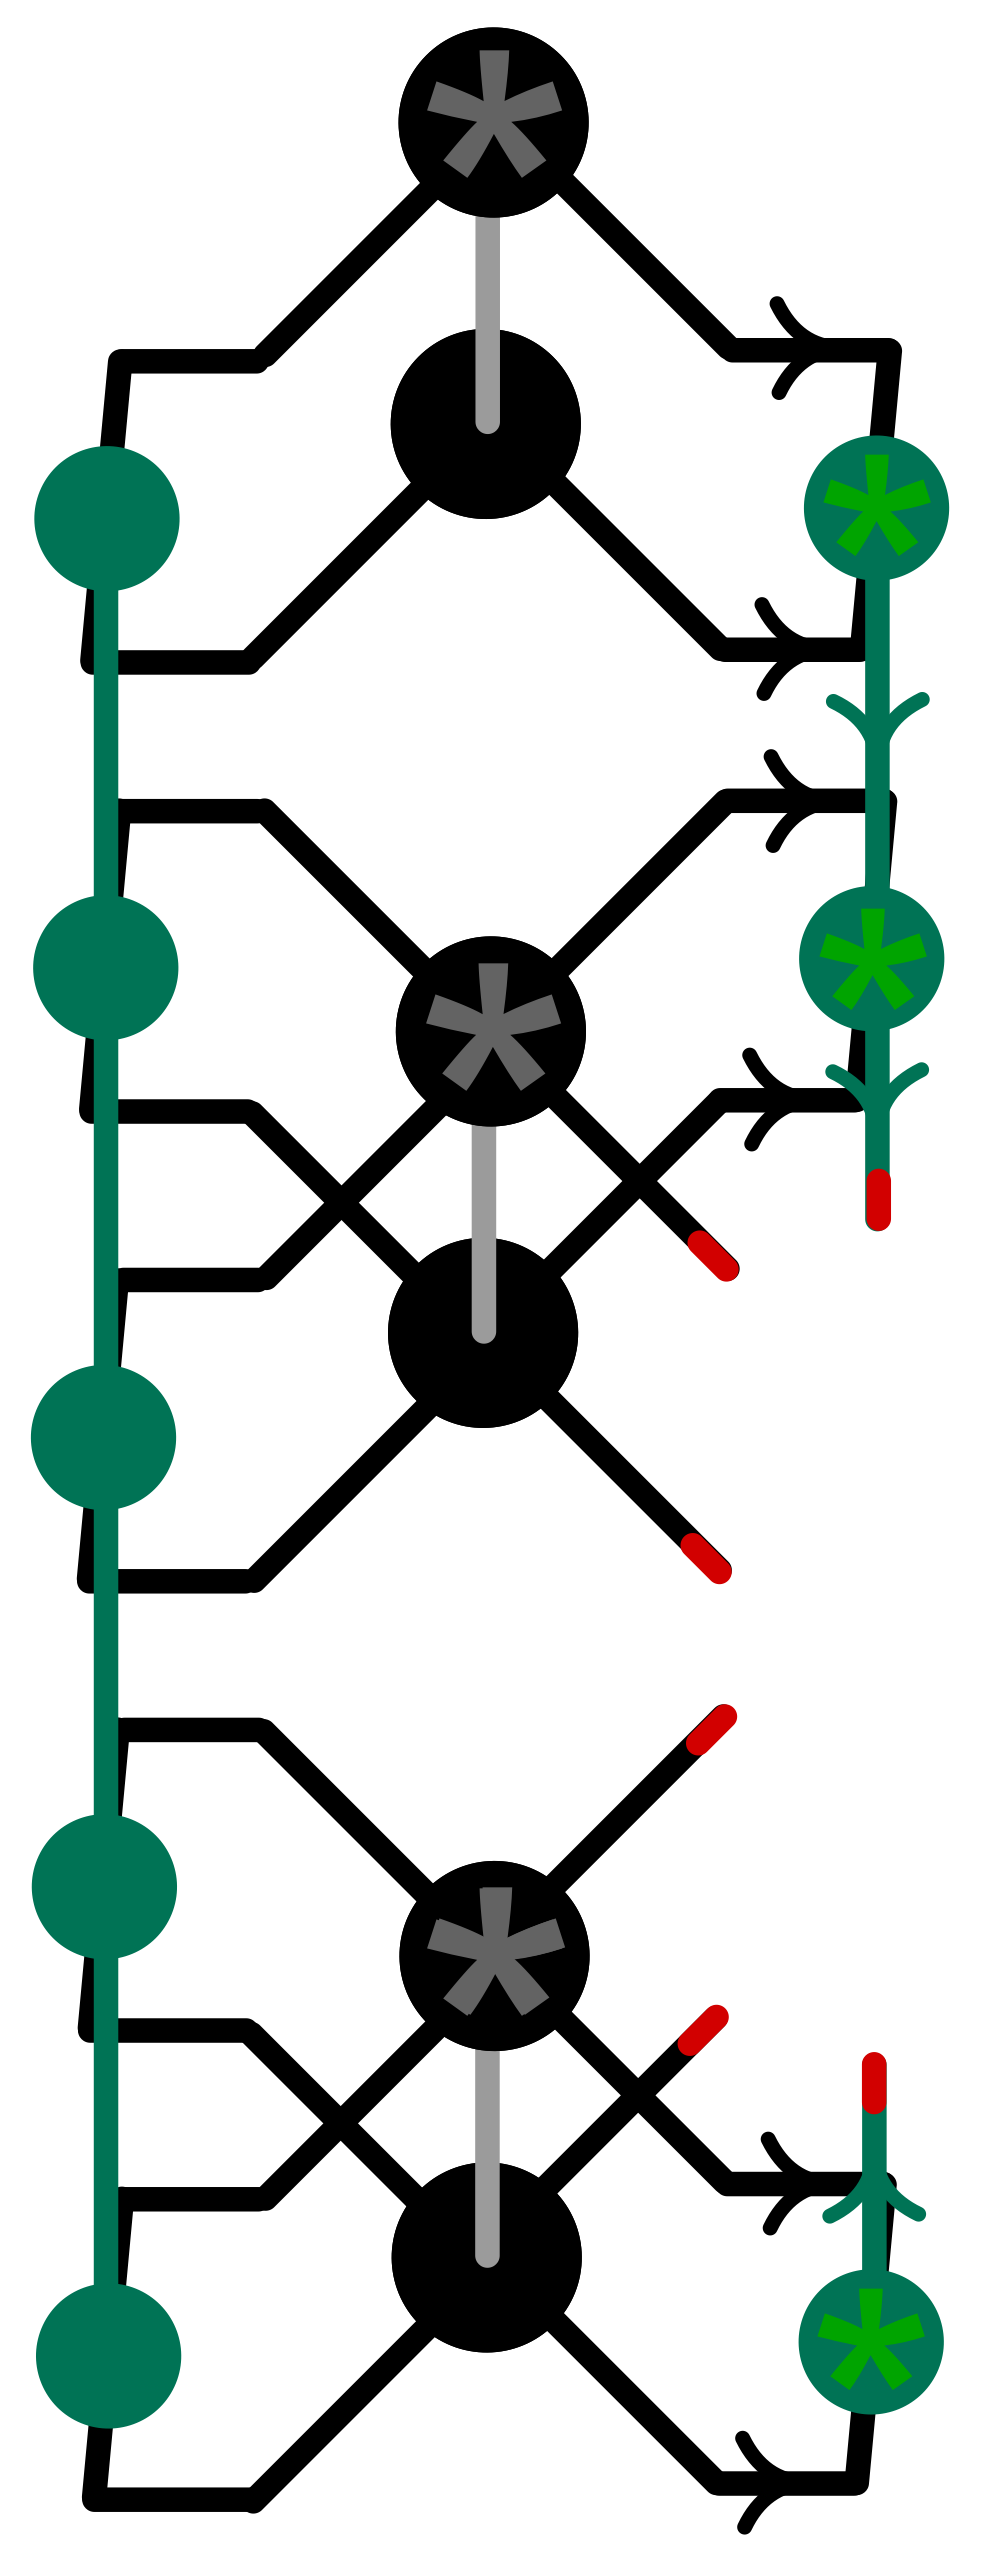
\includegraphics[height=4.2cm]{bc_theta_transfer.png}} \\
	\textstyle
	\left( L_h^{\text{transfer}} \middle\vert \partial_{\overline{\theta}_2} L_h(\overline{\theta}_2) \right)
	\end{array}
	=\:\:
	\raisebox{-0.47\height}{\includegraphics[height=2.4cm]{bc_theta.png}}.
\end{equation}
Note that $\theta_2$ contains the global norm $\Vert L_h \Vert$. We extract it before performing the truncated SVD, that splits $\theta_2^{[n_y, n_y+1]}$ into $U^{[n_y]}$, $S^{[n_y]}$ and $V^{[n_y+1]}$ and allows moving to the next site. We start from an initial random guess for $(L_h\vert$ and sweep up and down with the local updates \eqref{eq:bc_update_theta2} until the $\theta_2$s do not change significantly anymore. The most expensive part regarding computational runtime is the SVD with complexity
\begin{equation}
	\mathcal{O}( D_{\text{max}}^6 \: \chi_{\text{max}, b}^3 ).
\end{equation}

% bulk-weighted bc
\newpage
\noindent \underline{Bulk-weighted boundary compression} \\[0.5em]
Apart from the identity contractions of the $A_L$s left of $h$, the variational boundary compression \eqref{eq:bc_update_theta2} is a general PEPS procedure that does not explicitly use the isometric structure. We now want to develop a new compression method that does so, by weighting the boundary truncations according to the singular values contained in the orthogonality column. To be precise, we require $( L_h \vert$ and $(L_h^{\text{new}} \vert + (L_h^{\text{transfer}} \vert$ to (approximately) have the same expectation value with the double orthogonality column $\vert C \overline{C} )$ right next to them. Due to the isometric structure, the latter contains the entire information about the right bulk:
\begin{equation} \label{eq:bulk_weighted_bc}
	\begin{array}{c}
	\raisebox{-0.5\height}{\includegraphics[height=4.5cm]{Lh1_CCdagger.png}} \\
	\left( 
	\begin{array}{c}
	\overline{A}_L^{[n_x-1]} \overline{A}_L^{[n_x]} \\
	\textcolor{LimeGreen}{h^{[n_x-1, n_x]}} \\
	A_L^{[n_x-1]} A_L^{[n_x]}
	\end{array}
	\middle\vert 
	\begin{array}{c}
	\textcolor{blue}{\overline{C}^{[n_x]}} \\
	\textcolor{blue}{C^{[n_x]}}
	\end{array}
	\right)
	\end{array}
	\:+\:
	\begin{array}{c}
	\raisebox{-0.5\height}{\includegraphics[height=4.5cm]{Lh2_CCdagger.png}} \\
	\left( 
	\begin{array}{cc}
	& \overline{A}_L^{[n_x]} \\
	\textcolor{ForestGreen}{L_h^{[n_x-1]}} & \\
	& A_L^{[n_x]}
	\end{array}
	\middle\vert 
	\begin{array}{c}
	\textcolor{blue}{\overline{C}^{[n_x]}} \\
	\textcolor{blue}{C^{[n_x]}}
	\end{array}
	\right)
	\end{array}
	\: \approx \:
	\begin{array}{c}
	\raisebox{-0.5\height}{\includegraphics[height=4.2cm]{Lh_CCdagger.png}} \\
	\left( 
	\textcolor{ForestGreen}{L_h^{[n_x]}}
	\middle\vert 
	\begin{array}{c}
	\textcolor{blue}{\overline{C}^{[n_x]}} \\
	\textcolor{blue}{C^{[n_x]}}
	\end{array}
	\right)
	\end{array}.
\end{equation}
We first bring $(L_h^{\text{new}} \vert$, $(L_h^{\text{transfer}} \vert$ and $\vert C \overline{C} )$ in bMPS form with single tensor per site, via QR decomposition and leg merging:
\begin{equation}
	\raisebox{-0.5\height}{\includegraphics[height=2.2cm]{qr_Lh1.png}} \:\:,
	\hspace{2em}
	\raisebox{-0.5\height}{\includegraphics[height=2cm]{qr_Lh2.png}} \:\:,
	\hspace{2em}
	\raisebox{-0.5\height}{\includegraphics[height=2.3cm]{qr_CCdagger.png}}.
\end{equation}
We take $\vert C \overline{C} )$ in its thereby achieved down isometric form and discard its global norm. With this we can reformulate \eqref{eq:bulk_weighted_bc} as finding an $( L_h \vert$ that (a) has down isometric form, (b) global norm $\Vert L_h \Vert$, (c) maximal bond dimension $\chi_{\text{max}, b}$ and (d) fulfills
\begin{equation}
	\begin{array}{c}
	\raisebox{-0.5\height}{\includegraphics[height=4.5cm]{Lh1_C.png}} \\
	(\textcolor{IntenseLimeGreen}{L_h^{\text{new}}} \vert  \textcolor{IntenseCerulean}{C \overline{C}} )
	\end{array}
	\:+\:
	\begin{array}{c}
	\raisebox{-0.5\height}{\includegraphics[height=4.5cm]{Lh2_C.png}} \\
	(\textcolor{teal}{L_h^{\text{transfer}}} \vert \textcolor{IntenseCerulean}{C \overline{C}} )
	\end{array}
	\:\approx\:
	\begin{array}{c}
	\raisebox{-0.48\height}{\includegraphics[height=4.5cm]{Lh_C.png}} \\
	\hspace*{2em} ( \textcolor{ForestGreen}{L_h} \vert \textcolor{IntenseCerulean}{C \overline{C}} )
	\end{array}.
\end{equation}
From top to bottom, we compute the expectation values $(L_h^{\text{new}} \vert C \overline{C} )$ and $(L_h^{\text{transfer}} \vert C \overline{C} )$ site per site and save all partial contractions. Then, from bottom to top, i.e. for every $n_y = 1, \ldots, 2L_y-2$, we perform the following three steps, where we compactly denote "new" as "1" and "transfer" as "2", and omit the index $n_y$ for the tensors $L_h^{1[n_y]}$, $L_h^{2[n_y]}$ and $C\overline{C}^{[n_y]}$:
\begin{enumerate}
	\item[1)] Cut the two legs connecting $L_h^{1}$ and $L_h^{2}$ with $C\overline{C}$. Perform a "stacked QR decomposition" to split off a common down isometric Q. More precisely, stack the columns of $L_h^1$ and $L_h^2$ into a single matrix $( L_h^{1} \: L_h^{2})$, perform an ordinary QR decomposition $( L_h^{1} \: L_h^{2}) = QR$, and split the triangular matrix $R = (R_1 \: R_2)$ such that $Q R_1 = L_h^1$ and $Q R_2 = L_h^2$. Diagrammatically:
\begin{equation} \label{eq:stacked_qr}
	\raisebox{-0.5\height}{\includegraphics[height=2.2cm]{stacked_qr.png}} \:.
\end{equation}

	\item[2)] Absorb the triangular matrices $R_1$ and $R_2$ into the partial expectation values $L_h^1 C$ and $L_h^2 C$, which then have same dimensions and can be summed up to $L_h C$. Decompose $L_hC = U S V$ with SVD and truncate to $\chi_{\text{max}, b}$ (if the dimension of $S$ exceeds $\chi_{\text{max}, b}$). Between $U$ and $S$, insert an identity $U_{[:\chi_{\text{max}, b}, :]}^{\dagger} U_{[:, :\chi_{\text{max}, b}]} = \mathbbm{1}_{\chi_{\text{max}, b}}$:
\begin{equation}
	\raisebox{-0.5\height}{\includegraphics[height=4.5cm]{Lh1C.png}}
	\:\:+\:\:
	\raisebox{-0.5\height}{\includegraphics[height=4.5cm]{Lh2C.png}}
	\:\:=\:\:
	\raisebox{-0.5\height}{\includegraphics[height=4.5cm]{LhC.png}}
	\:\:
	\raisebox{-0.5\height}{\includegraphics[height=3.5cm]{svd_LhC.png}}.
\end{equation}

	\item[3)] Insert back $U_{[:, :\chi_{\text{max}, b}]} S_{[:\chi_{\text{max}, b}, :\chi_{\text{max}, b}]} V_{[:\chi_{\text{max}, b}, :]} \approx L_h C = L_h^1 C + L_h^2 C$. Contraction of $Q$ and $U_{[:, :\chi_{\text{max}, b}]}$ gives the common bMPS tensor $L_h$. Absorb $U^{\dagger}_{[:\chi_{\text{max}, b}, :]} R_1$ and $U^{\dagger}_{[:\chi_{\text{max}, b}, :]} R_2$ into $L_h^1$ and $L_h^2$ of the next site $n_y+1$:
\begin{equation}
	\raisebox{-0.5\height}{\includegraphics[height=5cm]{LhC_proj.png}}
	\:\:=\:\:
	\raisebox{-0.5\height}{\includegraphics[height=4.8cm]{Lh1C_proj.png}}
	\:\:+\:\:
	\raisebox{-0.5\height}{\includegraphics[height=4.8cm]{Lh2C_proj.png}}
	\:.
\end{equation}
\end{enumerate}
On the last site $n_y = 2L_y-1$, $R_1$ and $R_2$ are vectors and their sum contains the global norm $\Vert L_h \Vert$. The corresponding unit vector plays the role of $U$:
\begin{equation} \label{eq:bulk_weighted_bc_last_site}
	\raisebox{-0.5\height}{\includegraphics[height=2cm]{Lh_last_site.png}} \:.
\end{equation}

\begin{figure}[H]
  \centering
  \includegraphics[width=1.0\linewidth]{boundary_compression_6_6.png}
  \caption{Benchmark for the bulk-weighted boundary compression \eqref{eq:bulk_weighted_bc} in comparison to the standard variational compression \eqref{eq:bc_update_theta2}. For the orthogonality column on the right side of the isoPEPS, we compress all left bMPS \eqref{eq:Lh_bMPS} and compute the expectation value $E_{\text{bc}}$ according to \eqref{eq:E_bc}. For converged bMPS, we expect $E_{\text{bc}}$ to equal $E_{\text{YB}}$ \eqref{eq:E_YB} up to the error collected by the latter from sweeping through the state with Yang-Baxter moves. For isoPEPS with $L_x = L_y = 6$ and bond dimensions $D_{\text{max}} = 2, 3, 4, 5, 6$, we plot the relative energy differences against increasing boundary bond dimensions $\chi_{\text{max},b} = 6D_{\text{max}}^2$. A bullet $\bullet$ indicates that $E_{\text{bc}} - E_{\text{YB}} > 0$, while a cross $\times$ indicates that $E_{\text{bc}} - E_{\text{YB}} < 0$ (appears only twice for $D_{\text{max}} = 4, \chi_{\text{max},b} = 24$). The new bulk-weighted compression converges way quicker than the variational one. For the former, the converged energy differences get smaller with growing $D_{\text{max}}$ (as the YB errors do). For the latter, increasing $D_{\text{max}} > 4$ even worsens the energies, as all states in the growing variational space are weighted equally. We are in the paramagnetic phase of the TFI model. At (a) $g = 3.5$ (closer to product state) we reach slightly smaller energy differences than for (b) $g = 3.0$ (closer to critical point).}
\label{fig:bc}
\end{figure}

\noindent The stacked QR decomposition \eqref{eq:stacked_qr} has the highest asymptotic runtime complexity of 
\begin{equation}
	\mathcal{O}( D_{\text{max}}^6 \chi_{\text{max}, b}^3 ).
\end{equation}
% benchmark
\noindent \underline{Benchmark} \\[0.5em]
\noindent We now compare the performances of the two presented boundary compression methods. We apply them to approximate ground states obtained from a second order imaginary time $\text{TEBD}^2$ algorithm. The core idea is to implement the ground state projector $\lim_{t \to \infty} e^{-t H}$ in terms of local two-site gates. For this, we split time into $N$ small steps $\delta t$ and apply successive Suzuki-Trotter decompositions to the sum of column MPOs $H = \sum_{n_x} h^{[n_x, n_x +1]}$ \eqref{eq:column_mpo}:
\begin{align}
	&\ket{\psi_0} \propto \lim_{N \to \infty} \left( e^{-\delta t H} \right)^N \ket{\psi_{\text{init}}}, \\
	&e^{-\delta t H} \overset{\text{Suzuki-Trotter}}{=} \left( \prod_{n_x=1}^{2L_x-1} e^{-\frac{\delta t}{2} h^{[n_x, n_x +1]}} \right) \left( \prod_{n_x = 2L_x-1}^1 e^{-\frac{\delta t}{2} h^{[n_x, n_x +1]}} \right)+ \mathcal{O}(\delta t^3).
\end{align}
For each column evolution $e^{-\frac{\delta t}{2} h^{[n_x, n_x +1]}}$, we can then apply the well-established 1D TEBD scheme \cite{vidal2004efficient}. It splits $h$ into $h_{\text{odd}} + h_{\text{even}}$, where $h_{\text{odd}}$/$h_{\text{even}}$ is the sum of mutually commuting two-site gates acting on odd/even bonds. Another second order trotterization gives 
\begin{equation}
	e^{-\frac{\delta t}{2} h} \overset{\text{Suzuki-Trotter}}{=} e^{-\frac{\delta t}{4} h_{\text{odd}}} e^{-\frac{\delta t}{2} h_{\text{even}}} e^{-\frac{\delta t}{4} h_{\text{odd}}}+ \mathcal{O}(\delta t^3). 
\end{equation}
For further details we refer to \cite{sappler2024diagonal}, whose implementation we apply for $\delta t = 0.05$ and $N = 100$. \\

\noindent For converged boundaries $L_h$ and $R_h$, we expect $E_{\text{bc}}$ \eqref{eq:E_bc} and $E_{\text{YB}}$ \eqref{eq:E_YB} to be equal up to the energy error collected by the Yang-Baxter moves in $E_{\text{YB}}$. In figure \ref{fig:bc}, we plot the relative energy difference $\vert E_{\text{bc}} - E_{\text{YB}} \vert / \vert E_{\text{YB}} \vert$ against $\chi_{\text{max}, b}$ for $D_{\text{max}} = 2, 3, 4, 5, 6$. We can conclude:
\begin{itemize}
	\item The Yang-Baxter error gets smaller for larger bond dimension $D_{\text{max}}$ and we expect the converged energy difference between $E_{\text{YB}}$ and $E_{\text{bc}}$ to behave the same way. For the new bulk-weighted boundary compression \eqref{eq:bulk_weighted_bc}, this can be observed for all considered values of $D_{\text{max}}$. Convergence is reached quickly for increasing bMPS bond dimension $\chi_{\text{max}, b}$.
	\item In contrast, the standard variational boundary compression \eqref{eq:bc_update_theta2} does not converge within the covered range of $\chi_{\text{max}, b}$ for $D_{\text{max}} > 4$. The energies even get worse from $D_{\text{max}} = 4$ to $5$ and from $5$ to $6$. We give the following intuitive explanation: The "physical" bMPS legs have dimension up to $D_{\text{max}}^2$ each and thus the variational space in which we do the optimization grows as $D_{\text{max}}^{2(2L_y-1)}$. Since all states in the space are weighted equally by the variational compression, capturing a smaller fraction with growing $D_{\text{max}}$ leads to worse results. This was the main motivation for introducing the bulk-weighted compression scheme. 
\end{itemize}
For completeness we want to mention: When the boundaries \eqref{eq:Lh_bMPS} are not compressed additively but every column MPO term is compressed and transferred separately, the changes in figure \ref{fig:bc} are minor.


% DMRG^2
\section{Density matrix renormalization group squared ($\text{DMRG}^2$)} \label{sec:dmrg2}
To optimize the isoPEPS \eqref{eq:iso_peps} for the ground state of a Hamiltonian \eqref{eq:column_mpo}, we perform an algorithm that can be broken down into a high level sweep of column updates in x-direction, which unfold to a two-site DMRG in y-direction. Referring to this quadratic structure, it is called \textit{density matrix renormalization group squared} ($\text{DMRG}^2$) algorithm \cite{lin2022efficient}:
\begin{enumerate}
	\item[1)] Zero-column DMRG in $x$-direction \\[0.3em]
	Optimize the orthogonality column (which does not have any physical legs), while keeping all left and right isometric columns fixed. One update at center $n_x$ corresponds to finding the ground state column $\Tilde{C}^{[n_x]}$ of the effective Hamiltonian $H_{\text{eff},0}^{[n_x]}$ (with DMRG in y-direction as described in point 2 below):
\begin{align} \label{eq:dmrg2_column_update}
\begin{split}
	\raisebox{-0.5\height}{\includegraphics[height=3cm]{Heff0.png}} 
	\: = \: 
	\raisebox{-0.5\height}{\includegraphics[height=3cm]{Heff0_1.png}} 
	\: &+ \: 
	\raisebox{-0.5\height}{\includegraphics[height=3cm]{Heff0_2.png}} 
	\: + \: \raisebox{-0.5\height}{\includegraphics[height=3cm]{Heff0_3.png}} \\
	&\Downarrow \text{ground state} \\
	\textcolor{blue}{\tilde{C}^{[n_x-1]}} \tilde{A}_R^{[n_x]} A_R^{[n_x+1]} 
	\:\: \overset{\text{YB}}{\approx} \:\:
	A_L^{[n_x]} &\textcolor{blue}{\tilde{C}^{[n_x]}} A_R^{[n_x+1]} 
	\:\: \overset{\text{YB}}{\approx } \:\:
	A_L^{[n_x]} \tilde{A}_L^{[n_x+1]} \textcolor{blue}{\tilde{C}^{[n_x+1]}}
\end{split}
\end{align}
Move the updated orthogonality column right/left to $n_x+1$/$n_x-1$ with YB move. This indirectly also updates the involved isometric column to $\tilde{A}_L^{[n_x+1]}$/$\tilde{A}_R^{[n_x]}$. Compress the new bMPS $\tilde{L}_h^{[n_x+1]}$/$\tilde{R}_h^{[n_x]}$. The bulk-weighted boundary compression \eqref{eq:bulk_weighted_bc} seems to be sensitive also to propagated changes of $C$ and we find that going from local to global boundary updates stabilizes the algorithm vastly when using this scheme. With the described steps, repeatedly sweep $n_x = 0, \ldots, 2L_x$ left to right and back, until isoPEPS and energy converge. 

	\item[2)] Two-site DMRG in $y$-direction \\[0.3em]
	Perform the well-established 1D two-site DMRG as presented in section \ref{sec:dmrg}, but for the cMPS instead of a physical MPS. For an update of center $n_y$, start an iterative Lanczos algorithm with initial guess $\theta_2^{[n_y, n_y+1]}$ to find the ground state $\tilde{\theta}_2^{[n_y, n_y+1]}$ of the effective Hamiltonian. The action of the latter results from leaving out $\overline{\theta}_2^{[n_y, n_y+1]}$ in $E_{\text{bc}}$ \eqref{eq:E_bc}:
\begin{equation*}
	\raisebox{-0.5\height}{\includegraphics[height=3cm]{dmrg2_Heff.png}}
	\hspace{1.8em}=\hspace{1.8em}
	\raisebox{-0.5\height}{\includegraphics[height=4.2cm]{dmrg2_Heff_1.png}}
	\hspace{1.8em}+\hspace{1.8em}
	\raisebox{-0.5\height}{\includegraphics[height=5.2cm]{dmrg2_Heff_2.png}}
	\hspace{1.8em}+\hspace{1.8em}
	\raisebox{-0.5\height}{\includegraphics[height=4.2cm]{dmrg2_Heff_3.png}}
\end{equation*}
\vspace*{-1em}
\begin{equation} \label{eq:dmrg2_two_site_dmrg}
	\Downarrow \text{ground state}
\end{equation}
\begin{equation*}
	\:\:\raisebox{-0.5\height}{\includegraphics[height=2.2cm]{dmrg2_theta2_updated.png}} 
	\:\: \underset{\textcolor{blue}{\chi_{\text{max}, b}}}{\overset{\text{\textcolor{blue}{t}SVD}}{\approx}} \:\:
	\raisebox{-0.5\height}{\includegraphics[height=2.2cm]{dmrg2_theta2_split.png}} 
\end{equation*}
The truncated SVD $\tilde{\theta}_2^{[n_y, n_y+1]} \approx \tilde{U}^{[n_y]} \tilde{S}^{[n_y]} \tilde{V}^{[n_y+1]}$ allows to move one site up/down and perform the next ground state search with guess $\tilde{S}^{[n_y]} \tilde{V}^{[n_y+1]} V^{[n_y+2]}$/$U^{[n_y-1]}\tilde{U}^{[n_y]} \tilde{S}^{[n_y]}$. Sweep up and down along $n_y = 1, \ldots, 2L_y-2$ until the center tensors do not change significantly anymore.
\end{enumerate}
The multiplications with the effective boundary Hamiltonians have the maximum runtime complexity of
\begin{equation}
	\mathcal{O}( D_{\text{max}}^5 \chi_{\text{max}, c}^3 \chi_{\text{max}, b} ).
\end{equation}

\vspace*{2em}

\noindent \underline{Benchmark} \\[0.5em]
In figures \ref{fig:dmrg2_3.5_1}--\ref{fig:dmrg2_3.0_2} we run $\text{DMRG}^2$ in the paramagnetic phase of the TFI model, for $N = 72$ spins on a diagonal square lattice with $L_x = L_y = 6$. Relative to an MPS reference, we track the energy error before ($\bullet$) and after ($\times$) every column update \eqref{eq:dmrg2_column_update}. For the final state, we additionally compute the expectation value $E_{\text{YB}}$ (---). We can draw the following conclusions:
\begin{itemize}
	\item What we found for the energy expectation value in the last section (figure \ref{fig:bc}) also holds for its minimization with effective Hamiltonians: For $D_{\text{max}} \geq 4$, the newly developed bulk-weighted boundary compression \eqref{eq:bulk_weighted_bc} leads to significantly smaller errors than the variational compression \eqref{eq:bc_update_theta2}, which even gets worse from $D_{\text{max}} = 4$ to $5$ and from $5$ to $6$. We recall our understanding from the previous section: the dimension of the variational space in which the optimization is performed grows as $D_{\text{max}}^{2(2L_y-1)}$, while the maximal allowed bMPS bond dimension is $\chi_{\text{max}, b} = 6D_{\text{max}}^2$. Since all states in the space are weighted equally by the variational compression, capturing a smaller fraction with growing $D_{\text{max}}$ leads to worse results. This highlights the necessity of the improved bulk-weighted boundary compression method.
	\item The variational power of the isoPEPS is largest when the orthogonality column is located at the center of the lattice, from where the energies increase towards the edges. This can be explained by the enlarged bond dimension $\chi_{\text{max}, c} = 6D_{\text{max}}$ on the orthogonality column, which has the strongest global effect on the isometric tensors when positioned in their middle. This behavior is smoothed out when reducing $\chi_{\text{max}, c}$, as demonstrated in figure \ref{fig:dmrg2_3.5_3} for $\chi_{\text{max}, c} = 3D_{\text{max}}$. The final expectation value $E_{\text{YB}}$, which is received from moving the orthogonality column through the entire state, is almost not affected by the reduction of $\chi_{\text{max}, c}$.
\end{itemize}
\noindent The further discussion refers to $\text{DMRG}^2$ with the bulk-weighted boundary compression.
\begin{itemize}
	\item Deep in the paramagnetic phase ($g = 3.5$), isoPEPS bond dimensions $D_{\text{max}} > 4$ do not further lower the energies. This changes, at least for $D_{\text{max}} = 5$, when approaching the critical point ($g = 3.0$), whereby the ground state entanglement grows. 
	\item For figures \ref{fig:dmrg2_3.5_1}--\ref{fig:dmrg2_3.0_1} we choose a bMPS bond dimension $\chi_{\text{max}, b} = 6D_{\text{max}}^2$. The fast convergence of the expectation value in figure \ref{fig:bc} suggests that a smaller bond dimension would give similarly good results. In figure \ref{fig:dmrg2_3.0_2} we halve the value to $\chi_{\text{max}, b} = 3D_{\text{max}}^2$. For  $D_{\text{max}} = 2, 3, 4$, the differences relative to figure \ref{fig:dmrg2_3.0_1} are indeed minor. For  $D_{\text{max}} = 5$, the final expectation value gets slightly worse. Note that smaller errors for some energies after column DMRG ($\times$) can be misleading. In fact, the errors have negative sign, indicating an inaccurate compression of the effective Hamiltonian, since the true ground state must have the smallest energy in the whole Hilbert space.
\end{itemize}

\newpage
\vspace*{\fill}
\begin{figure}[H]
  \centering
  \includegraphics[width=1.0\linewidth]{dmrg_6_6_3.5_1.png}
  \caption{TFI Benchmark for $\text{DMRG}^2$ with (a) the new bulk-weighted boundary compression and (b) variational boundary compression. We optimize an isoPEPS on a diagonal square lattice of $L_x = L_y = 6$ for the ground state of the TFI model at $g = 3.5$. Relative to an MPS reference ($E_0$), we plot the energy error before ($\bullet$) and after ($\times$) every column update \eqref{eq:dmrg2_column_update}, and the final error for the expectation value $\langle H \rangle = E_{\text{YB}}$ (---). While for $D_{\text{max}} = 2, 3$ both boundary compression methods reach the same energies, the new bulk-weighted compression outperforms the variational one for $D_{\text{max}} = 4$. As can be seen in figure \ref{fig:dmrg2_3.5_2}, $D_{\text{max}} = 5, 6$ do not lower the energies further. We choose $\chi_{\text{max},b} = 6D_{\text{max}}^2$ and a relatively high orthogonality column bond dimension $\chi_{\text{max},c} = 6D_{\text{max}}$. The latter enlarges the variational power when the orthogonality column is located in the center of the lattice, from where the energies go up towards the edges. Reducing $\chi_{\text{max},c}$ smoothens out these differences, as can be observed in figure \ref{fig:dmrg2_3.5_3} for $\chi_{\text{max}, c} = 3D_{\text{max}}$.}
\label{fig:dmrg2_3.5_1}
\end{figure}
\vspace*{\fill}

\newpage
\vspace*{\fill}
\begin{figure}[H]
  \centering
  \includegraphics[width=1.0\linewidth]{dmrg_6_6_3.5_2.png}
  \caption{Continuation of figure \ref{fig:dmrg2_3.5_1} for $D_{\text{max}} = 5, 6$. The data for $D_{\text{max}} = 4$ is plotted again for reference. For (a) the new bulk-weighted boundary compression, the final energy errors remain close to the value obtained for $D_{\text{max}} = 4$. For (b) variational compression, the bMPS with bond dimensions $\chi_{\text{max},b} = 6D_{\text{max}}^2$ capture the effective Hamiltonian worse and worse for $D_{\text{max}} > 4$.}
 \label{fig:dmrg2_3.5_2}
\end{figure}
\vspace*{\fill}

\newpage
\vspace*{\fill}
\begin{figure}[H]
  \centering
  \includegraphics[width=1.0\linewidth]{dmrg_6_6_3.5_3.png}
  \caption{$\text{DMRG}^2$ with reduced bond dimension on the orthogonality column. We halve the value from $\chi_{\text{max}, c} = 6D_{\text{max}}$ in figure \ref{fig:dmrg2_3.5_1} to $\chi_{\text{max}, c} = 3D_{\text{max}}$ and compare the second half of the three column sweeps. As expected, the reduction smoothens out the differences in variational power for the orthogonality column located in the center vs. at the edges.}
\label{fig:dmrg2_3.5_3}
\end{figure}
\vspace*{\fill}

\newpage
\vspace*{\fill}
\begin{figure}[H]
  \centering
  \includegraphics[width=1.0\linewidth]{dmrg_6_6_3.0_1.png}
  \caption{$\text{DMRG}^2$ closer to the critical point. We move from $g = 3.5$ in figure \ref{fig:dmrg2_3.5_1} to $g = 3.0$ in this figure. The critical point in the thermodynamic limit is $g_c \approx 3.044$, but for the chosen diagonal square lattice with $L_x = L_y = 6$ and OBC we are still in the paramagnetic phase. Nevertheless, the ground state entanglement is higher so that $D_{\text{max}} = 5$ further lowers the energy compared to $D_{\text{max}} = 4$, at least when using (a) the new bulk-weighted boundary compression. For (b) the standard variational boundary compression, the final expectation value errors for $D_{\text{max}} = 4$ and $5$ are on the same level and higher than the ones for (a).}
\label{fig:dmrg2_3.0_1}
\end{figure}
\vspace*{\fill}

\newpage
\vspace*{\fill}
\begin{figure}[H]
  \centering
  \includegraphics[width=1.0\linewidth]{dmrg_6_6_3.0_2.png}
  \caption{$\text{DMRG}^2$ with reduced bMPS bond dimension. We halve the value from $\chi_{\text{max}, b} = 6D_{\text{max}}^2$ in figure \ref{fig:dmrg2_3.0_1} to $3D_{\text{max}}^2$ and compare the second half of the three column sweeps. While for $D_{\text{max}} = 2, 3, 4$ the differences are minor, the final expectation value $\langle H \rangle$ (---) slightly worsens for $D_{\text{max}} = 5$. In (a), the smaller errors for some effective ground state energies ($\times$) can be misleading. In fact, the errors have negative sign, indicating an inaccurate compression of the effective Hamiltonian, since the true ground state must have the smallest energy ($E_0$) in the whole Hilbert space.}
\label{fig:dmrg2_3.0_2}
\end{figure}
\vspace*{\fill}

% VARIATIONAL QUASIPARTICLE EXCITATIONS
\newpage
\section{Variational quasiparticle excitations} \label{sec:vqpe2}
In a similar fashion as for MPS in section \ref{sec:vqpe}, we now want to create quasiparticle excitations against the correlated isoPEPS ground state vacuum. Again (but as we will see, less strictly), a tangent space vector serves as orientation. It results from small deviations from the isoPEPS that has, by our convention, the orthogonality column on the very right:
\begin{equation} \label{eq:iso_peps_AL_C}
	\ket{\psi(A_L, C)} 
	\:=\:
	\raisebox{-0.5\height}{\includegraphics[height=5cm]{iso_peps_AL_C.png}} .
\end{equation}
In contrast to the MPS \eqref{eq:canonical_form_mps} with $C^{[N]} = ((1)) \in \mathbb{C}^{1 \times 1}$, the orthogonality column $C^{[2L_x]} \in \mathbb{C}^{D_{\text{max}}^{2L_y-1} \times 1}$ in \eqref{eq:iso_peps_AL_C} is nontrivial. As a consequence, we additionally have to take into account the derivative after each of its components when building the tangent space vector:
\begin{align} \label{eq:iso_peps_tangent_vector}
\begin{split} 
	&\ket{\psi(B, D; A_L, C)} \\
	&= \sum_{n_x, y} \sum_{s, \alpha, \beta, \gamma, \delta} B^{[n_x, y]s}_{\alpha\beta\gamma\delta}
	\left[ \partial_{{\left(A_L^{[n_x,y]}\right)}^{s}_{\alpha\beta\gamma\delta}} \ket{\psi(A_L, C)} \right]
	+ \sum_{n_y} \sum_{d, l, r, u} D^{[n_y]}_{dlru} \left[ \partial_{C^{[2L_x, n_y]}_{dlru}} \ket{\psi(A_L, C)} \right] \\
	&= \sum_{n_x, y} \raisebox{-0.5\height}{\includegraphics[height=4cm]{tangent_iso_peps_1.png}} 
	\:+\:
	\sum_{n_y} \raisebox{-0.5\height}{\includegraphics[height=4cm]{tangent_iso_peps_2.png}} .
\end{split}
\end{align}

\noindent \underline{Parametrization of the ansatz} \\[0.5em]
We now want to parametrize the tangent space vector \eqref{eq:iso_peps_tangent_vector}---for a given ground state equivalently the perturbation tensors $B$, $D$---by a joint collection of tensors $X$, such that the individual states in the superposition
\begin{equation}
	\ket{\psi(X; A_L, C)} = \sum_{n_x, y} \ket{\psi(X^{[n_x, y]}; A_L, C)} + \sum_{n_y} \ket{\psi(X^{[n_y]}; A_L, C)}
\end{equation}
fulfill the following orthogonality conditions:
\begin{equation} \label{eq:e_iso_peps_properties}
	\begin{array}{ll}
	\text{1) Ground state} 
	&\langle \psi( \overline{A}_L, \overline{C}) \vert \psi(X^{[n_x, y]}; A_L, C) \rangle
	= \langle \psi( \overline{A}_L, \overline{C}) \vert \psi(X^{[n_y]}; A_L, C) \rangle
	= 0. \\[0.5em]
	\text{2) Pairwise}
	& \text{a)}\: \langle \psi(\overline{X}^{[n_x, y]};  \overline{A}_L, \overline{C}) \vert \psi(X^{[n_y]}; A_L, C) \rangle = 0, \\[0.3em]
	& \text{b)}\:\langle \psi(\overline{X}^{[\tilde{n}_x, \tilde{y}]};  \overline{A}_L, \overline{C}) \vert \psi(X^{[n_x, y]}; A_L, C) \rangle = \delta_{n_x, \tilde{n}_x} \delta_{y, \tilde{y}}(\overline{X}^{[n_x, y]} \vert X^{[n_x, y]}), \\[0.3em]
	& \text{c)}\: \langle \psi(\overline{X}^{[\tilde{n}_y]};  \overline{A}_L, \overline{C}) \vert \psi(X^{[n_y]}; A_L, C) \rangle = \delta_{n_y, \tilde{n}_y} (\overline{X}^{[n_y]} \vert X^{[n_y]}).
	\end{array}
\end{equation}
Property 1) enforces the physical requirement that the quasiparticle ansatz must be orthogonal to the ground state vacuum in order to describe a genuine excitation eigenstate. Property 2) makes the norm matrix equal the identity, which simplifies the variational eigenvalue problem and improves numerical stability. For MPS, it is a nice feature that these properties can be ensured exactly within the gauge freedom. This is not the case for isoPEPS. Fixing the gauge in general only removes null vectors, which makes the effective norm matrix positive definite (invertible). For \eqref{eq:iso_peps_tangent_vector}, $A_L$-perturbations of the form
\begin{equation} \label{eq:e_iso_peps_gauge}
	\begin{array}{ccl}
	B_0 &=  &A_L (X_d \otimes \mathbbm{1}_u) + A_L (\mathbbm{1}_d \otimes X_u) \\[0.5em]
	& & \text{with } X_d \in \mathbb{C}^{D_{rd} \times D_{rd}}, X_u \in \mathbb{C}^{D_{ru} \times D_{ru}}
	\end{array}
	\hspace{1em} \raisebox{-0.45\height}{\includegraphics[height=2.5cm]{AL_Xd.png}} + \raisebox{-0.45\height}{\includegraphics[height=2.5cm]{AL_Xu.png}} 
\end{equation}
can be subtracted on the next column. Since $(X_d, X_u) = (\alpha \mathbbm{1}_d, \beta \mathbbm{1}_u)$ and $(\beta \mathbbm{1}_d, \alpha \mathbbm{1}_u)$ give the same $B_0$, we effectively have $D_{rd}^2 + D_{ru}^2 - 1$ gauge parameters per tensor\footnote{Due to the closed loops in the virtual legs, there could be further gauge transformations that are not as obvious to write down as \eqref{eq:e_iso_peps_gauge}.}. However, to meet the desired properties \eqref{eq:e_iso_peps_properties} (to be precise, for now only 1, 2a and orthogonality of 2b), we have to project out deviation tensors of the form
\begin{equation} \label{eq:e_iso_peps_gauge_plus}
	\begin{array}{ccl}
	B_{0}^{+} &= &A_L X_{du} \\[0.5em]
	&& \text{with } X_{du} \in \mathbb{C}^{D_{rd}D_{ru} \times D_{rd}D_{ru}}
	\end{array}
	\hspace{1em} \raisebox{-0.45\height}{\includegraphics[height=2.5cm]{AL_Xdu.png}} \:.
\end{equation}
This fixes $D_{rd}^2D_{ru}^2$ parameters and is as restrictive as \eqref{eq:e_iso_peps_gauge} if $D_{rd} = 1$ or $D_{ru} = 1$, and more restrictive than \eqref{eq:e_iso_peps_gauge} if $D_{rd}, D_{ru} \geq 2$. In principle, we would like to span the whole tangent space and stick to gauging out \eqref{eq:e_iso_peps_gauge}, but for the excitation ansatz the practical benefits of \eqref{eq:e_iso_peps_properties} prevail. To remove \eqref{eq:e_iso_peps_gauge_plus}, we set $B^{[n_x, y]} = 0$ if $D_{ld}D_{lu}d = D_{rd}D_{ru}$ and
\begin{equation} \label{eq:e_iso_peps_VL}
	\text{ if } \textcolor{purple}{D_{ld}D_{lu}d - D_{rd}D_{ru}} > 0: \:\: 
	B^{[n_x, y]} \:\:=\:\: \raisebox{-0.6\height}{\includegraphics[height=2cm]{VL_X_gauge.png}} 
	\hspace{1em} \text{ with } \hspace{1em} \raisebox{-0.42\height}{\includegraphics[height=2.4cm]{VL_AL.png}} = 0.
\end{equation}
To make sure that the missing part of 2b), $\langle \psi(\overline{X}^{[n_x, y]}) \vert \psi(X^{[n_x, y]}) \rangle = (\overline{X}^{[n_x, y]} \vert X^{[n_x, y]})$, holds, we (approximately) move the orthogonality column right next to $X^{[n_x, y]}$ with YB moves, and absorb the two adjacent $C^{[n_x]}$-tensors (that together are normalized) therein. Compared to \eqref{eq:e_iso_peps_VL} this enlarges the variational space:
\begin{equation} \label{eq:e_iso_peps_VL_plus}
	\text{ if } \textcolor{purple}{D_{ld}D_{lu}d - D_{rd}D_{ru}} > 0: \:\:
	B^{[n_x, y]} \:\:=\:\: \raisebox{-0.45\height}{\includegraphics[height=2.3cm]{VL_X.png}} 
	\hspace{1em} \text{ with } \hspace{1em} \raisebox{-0.42\height}{\includegraphics[height=2.4cm]{VL_AL.png}} = 0.
\end{equation}
It remains to fix the gauge for the excitations $D$ on the orthogonality column $C^{[2Lx]}$, which we treat as a cMPS for this purpose. After having brought it into canonical form, the steps are completely analogous to the one we described for the MPS in equations \eqref{eq:excitation_gauge}--\eqref{eq:norm_excitation}, when we assign $C_D^{[n_y]}$ the role of $A_L^{[n]}$. Accordingly, we set $D^{[n_y]} = 0$ if $ \chi_d D_l D_r = \chi_u$ and
\begin{equation} \label{eq:e_iso_peps_VD}
	\text{ if } \textcolor{purple}{\chi_d D_l D_r - \chi_u} > 0: \:\:
	D^{[n_y]} \:\:=\:\: \raisebox{-0.3\height}{\includegraphics[height=2.6cm]{VD_X.png}} 
	\hspace{1em} \text{ with } \hspace{1em} \raisebox{-0.41\height}{\includegraphics[height=1.9cm]{VD_CD.png}} = 0.
\end{equation}
This guarantees 2c) and the second equality of 1) in \eqref{eq:e_iso_peps_properties}. In total, the parametrizations \eqref{eq:e_iso_peps_VL_plus} and \eqref{eq:e_iso_peps_VD} ensure that the desired properties \eqref{eq:e_iso_peps_properties} are fulfilled by the corresponding excitation ansatz $\ket{\psi(X; A_L, C)}$. The latter has the diagrammatic representation
\begin{equation} \label{eq:e_iso_peps}
	\ket{\psi(X; A_L, C)} 
	\:=\:
	\sum_{n_x, y}
	\raisebox{-0.5\height}{\includegraphics[height=4cm]{e_iso_peps_1.png}} 
	\:+\:
	\sum_{n_y}
	\raisebox{-0.5\height}{\includegraphics[height=4cm]{e_iso_peps_2.png}} 
	\:.
\end{equation}
We investigate the variational power of \eqref{eq:e_iso_peps} to capture quasiparticle excitations in two steps: 
\begin{enumerate}
	\item[1)] \vspace*{-0.15em} Overlap optimization\footnote{There are two equivalent ways to define the optimization: (i) $\argmin_X \Vert \text{isoPEPS}(X) - \psi \Vert^2$, where normalization is implicit in the cost function, or (ii) $\argmax_X \langle \text{isoPEPS}(\overline{X})\vert \psi \rangle$ subject to $\langle \text{isoPEPS}(\overline{X})\vert \text{isoPEPS}(X)\rangle = 1$. In the latter case a Lagrange multiplier enforces normalization, and both formulations lead to the stationarity condition $X = \partial_{\overline{X}} \langle \text{isoPEPS}(\overline{X}) \vert \psi \rangle$.} with the exact wavefunction or an MPS, 
	\item[2)] \vspace*{-0.5em} Diagonalization of the effective Hamiltonian. 
\end{enumerate}
\vspace*{-0.15em}
In the following we omit the explicit ground state reference $(A_L, C)$ in $\ket{\psi(X; A_L, C)} $ and write isoPEPS instead of $\psi$ when we want to clearly distinguish our ansatz from an exact wavefunction or MPS. \\[0.3em]

% from wavefunction overlap
\noindent \underline{From wavefunction overlap} \\[0.5em]
After having computed a full excitation wavefunction $\ket{\psi}$ with exact diagonalization (ED), the optimal local perturbation of the ground state isoPEPS at site $[n_x, y]$, in order to approximate $\ket{\psi}$, is given by
\begin{equation} \label{eq:_excitation_overlap_wavefunction}
	X^{[n_x, y]}_{\psi} 
	= \partial_{\overline{X}^{[n_x, y]}} \langle \text{isoPEPS}(\overline{X}) \vert \textcolor{magenta}{\psi} \rangle
	= \raisebox{-0.5\height}{\includegraphics[height=4.5cm]{overlap_wavefunction.png}} .
\end{equation}
Excitations on the orthogonality column are obtained analogously, by leaving the legs of $\overline{X}^{[n_y]}$ open. The achieved overlap does not need to be computed separately, but is equal to the squared norm of the optimized parameters:
\begin{align} \label{eq:overlap_normX}
\begin{split}
	 \langle \text{isoPEPS}(\overline{X}) \vert \textcolor{magenta}{\psi} \rangle
	 &=
	 \sum_{n_x, y} \langle \text{isoPEPS}(\overline{X}^{[n_x, y]}) \vert \textcolor{magenta}{\psi} \rangle
	 +
	 \sum_{n_y} \langle \text{isoPEPS}(\overline{X}^{[n_y]}) \vert \textcolor{magenta}{\psi} \rangle
	 \\
	 &=
	 \sum_{n_x, y} (\overline{X}^{[n_x, y]}\vert \underbrace{\partial_{\overline{X}^{[n_x, y]}} \langle \text{isoPEPS}(\overline{X}) \vert \textcolor{magenta}{\psi} \rangle}_{= \vert X^{[n_x, y]})}
	 +
	 \sum_{n_y} (\overline{X}^{[n_y]}\vert \underbrace{\partial_{\overline{X}^{[n_y]}}\langle \text{isoPEPS}(\overline{X}) \vert \textcolor{magenta}{\psi} \rangle}_{= \vert X^{[n_y]})}
	 \\
	 &= \sum_{n_x, y} \Vert X^{[n_x, y]} \Vert^2 + \sum_{n_y} \Vert X^{[n_y]} \Vert^2 = \Vert X \Vert^2.
\end{split}
\end{align}
This approach is restricted to small systems of $N \lesssim 20$ spin-1/2s and thus to $L_x, L_y \lesssim 3$ for the diagonal square lattice. \\[1em]

% from mps overlap
\noindent \underline{From MPS overlap} \\[0.5em]
For larger systems, where ED is no longer feasible, we can instead wind an MPS through the square lattice and run DMRG + VQPE. The corresponding isoPEPS excitations to maximize the overlap are given by
\begin{equation} \label{eq:_excitation_overlap_mps}
	X^{[n_x, y]}_{\text{MPS}}
	= \textcolor{magenta}{\sum_{n=1}^{2L_xL_y}} \partial_{\overline{X}^{[n_x, y]}} 
	\langle \text{isoPEPS}(\overline{X}) \vert \text{MPS}(\textcolor{magenta}{B^{[n]}}) \rangle
	= \textcolor{magenta}{\sum_{n=1}^{2L_xL_y}} \raisebox{-0.5\height}{\includegraphics[height=4.5cm]{overlap_mps.png}} .
\end{equation}
For each term in the sum, we contract the isoPEPS tensors column per column with the MPS tensors, separately from left and from right until we reach the open legs. In this way, the intermediate boundary tensors carry $2 L_y - 1$ open legs of maximal dimension $D_{\text{max}}$. The required memory scales exponentially as $\mathcal{O}(D_{\text{max}}^{2 L_y - 1})$, which is the key limitation of this procedure. The interaction range of the Hamiltonian is $L_y + 1$ for our choice of MPS winding. Accordingly, the required virtual bond dimension of the MPS, which appears as additional factor in the boundary dimension, increases with $L_y$. We go up to a parameter combination of $L_x = L_y = 5$, $D_{\text{max}}^{\text{MPS}} = 256$ and $D_{\text{max}} = 3$. Relation \eqref{eq:overlap_normX} again holds, providing the achieved overlap without extra computation. \\[1em]

% from effective hamiltonian
\noindent \underline{From effective Hamiltonian} \\[0.5em]
Finally, we optimize the excitation parameters $X$ energetically by solving the eigenvalue problem $H_{\text{eff}} \vert X ) = \lambda \vert X )$. We implement the matrix-vector multiplication $\vert \tilde{X} ) = H_{\text{eff}} \vert X )$ by performing a conversion
\begin{equation} \label{eq:X_to_single_B}
	X = \{X^{[n_x, y]}, X^{[n_y]}\}_{n_x, y, n_y} 
	\:\rightarrow\:
	B = \{B^{[n_x, y]}\}_{n_x, y},
\end{equation}
computing
\begin{equation} \label{eq:Heff_B_eigenequation}
	\vert \tilde{B} )^{[n_x, y]}
	= 
	\partial_{\overline{B}^{[n_x, y]}} \langle \psi(\overline{B}) \vert H \vert \psi(B) \rangle
\end{equation}
and transforming back to $\vert \tilde{X} )$ with the inverse of \eqref{eq:X_to_single_B}. Latter we can do locally thanks to the orthogonality conditions \eqref{eq:e_iso_peps_properties}. For all $n_x = 1, \ldots, 2L_x-1$, we take the $B$-tensors as already defined in \eqref{eq:e_iso_peps_VL_plus}:
\begin{equation} 
	\begin{array}{c}
	\raisebox{-0.5\height}{\includegraphics[height=2cm]{B.png}} \\
	B^{[n_x, y]} 
	\end{array}
	\:=\:
	\begin{array}{c}
	\raisebox{-0.5\height}{\includegraphics[height=2cm]{B1.png}} \\
	V_L^{[n_x, y]} X^{[n_x, y]}
	\end{array}
	\hspace{1em} (n_x = 1, \ldots, 2L_x-1).
\end{equation}
On the last column $n_x = 2L_x$, we additionally include the excitations on the orthogonality column:
\begin{equation}
	\begin{array}{c}
	\raisebox{-0.5\height}{\includegraphics[height=2cm]{B.png}} \\
	B^{[2L_x, y]} 
	\end{array}
	\:=\:
	\begin{array}{c}
	\raisebox{-0.5\height}{\includegraphics[height=2cm]{B1.png}} \\
	V_L^{[2L_x, y]} X^{[2L_x, y]}
	\end{array}
	+
	\begin{array}{c}
	\raisebox{-0.5\height}{\includegraphics[height=2cm]{B2.png}} \\
	A_L^{[2L_x, y]}
	\begin{array}{c}
	X^{[2y-1]} \\
	V_D^{[2y-1]}
	\end{array}
	\end{array}
	+
	\begin{array}{c}
	\raisebox{-0.5\height}{\includegraphics[height=2.1cm]{B3.png}} \\
	A_L^{[2L_x, y]}
	\begin{array}{c}
	X^{[2y]} \\
	V_D^{[2y]} 
	\end{array}
	\end{array}.
\end{equation}
Inversely, the two excitation types can be separated by contracting $B^{[2L_x, y]}$ with $\overline{V}_L^{[2L_x, y]}$/$\overline{A}_L^{[2L_x, y]}$, which projects out the $A_L^{[2L_x, y]}$/$V_L^{[2L_x, y]}$ terms. On the cMPS, the analogous orthonormality properties of the $C_D$s and $V_D$s can be used to extract $X^{[2y-1]}$ and $X^{[2y]}$. \\[0.5em]

\noindent Moreover, with the help of a finite state machine (FSM), we can capture the sum in y-direction with a single set of MPO-like tensors that have doubled vertical bond dimension:
\begin{align} \label{eq:B_column}
\begin{split}
	B^{[n_x]} \:\:=\:\: \sum_{y=1}^{L_y} \raisebox{-0.5\height}{\includegraphics[height=5cm]{AD_B_AU.png}} 
	\begin{array}{c}
	A_U^{[n_x, y+1]} \\[2.8em]
	B^{[n_x, y]} \\[2.8em]
	A_D^{[n_x, y-1]}
	\end{array}
	\:\:=\:\: &\raisebox{-0.5\height}{\includegraphics[height=4cm]{B_sum.png}} \hspace{0.5em} \\
	& \downarrow \text{FSM} \\
	\scriptstyle
	\bordermatrix{~ & \textcolor{purple}{\textstyle \chi_u} & \textcolor{purple}{\textstyle \chi_u} \cr
              		     \textcolor{purple}{\textstyle \chi_d} & A_D^{[n_x, 1]} & B^{[n_x, 1]}}, \hspace{1em}
	&\bordermatrix{~ & \textcolor{purple}{\textstyle \chi_u} & \textcolor{purple}{\textstyle \chi_u} \cr
              		     \textcolor{purple}{\textstyle \chi_d} & A_D^{[n_x, y]} & B^{[n_x, y]} \cr
		     	     \textcolor{purple}{\textstyle \chi_d} & 0 & A_U^{[n_x, y]}}_{y = 2, \ldots, L_y-1}, \hspace{1em}	
	\bordermatrix{~ & \textcolor{purple}{\textstyle \chi_u} \cr
              		     \textcolor{purple}{\textstyle \chi_d} & B^{[n_x, L_y]} \cr
		     	     \textcolor{purple}{\textstyle \chi_d} & A_U^{[n_x, L_y]}} .
\end{split}
\end{align}
With \eqref{eq:B_column}, the isoPEPS excitation ket \eqref{eq:e_iso_peps} has the compact diagrammatic representation
\begin{equation} \label{eq:ket_B}
	\ket{\psi(B)} = \sum_{n_x=1}^{2L_x} \ket{\psi(B^{[n_x]})} 
	\:=\: \raisebox{-0.5\height}{\includegraphics[height=3cm]{psiB_1.png}}
	\:+\:
	\raisebox{-0.5\height}{\includegraphics[height=3cm]{psiB_2.png}}
	\:+\: \ldots \:+\:
	\raisebox{-0.5\height}{\includegraphics[height=3cm]{psiB_3.png}} .
\end{equation}
In accordance with this notation, we draw the bra derivative in \eqref{eq:Heff_B_eigenequation} as
\begin{equation} \label{eq:deriv_bra}
	\partial_{\overline{B}^{[n_x, y]}} \langle \psi(\overline{B}) \vert 
	\:=\:
	\raisebox{-0.5\height}{\includegraphics[height=3.2cm]{deriv_bra_1.png}} 
	\:=\:
	\raisebox{-0.5\height}{\includegraphics[height=3.2cm]{deriv_bra_2.png}} .
\end{equation}
Sandwiching the Hamiltonian \eqref{eq:column_mpo} between \eqref{eq:ket_B} and \eqref{eq:deriv_bra}, gives an action of the effective Hamiltonian as specified on the next page in equation \eqref{eq:Heff_B}. The terms that vanish due to the orthogonality properties implied by \eqref{eq:e_iso_peps_VL_plus} and \eqref{eq:e_iso_peps_VD} are already omitted. The double sum over $H = \sum_{\tilde{n}_x} h^{[\tilde{n}_x, \tilde{n}_x+1]}$ and $\ket{\psi(B)} = \sum_{n_x^{\prime}} \ket{\psi(B^{[n_x^{\prime}]})}$ is covered by the rows and columns of the orange boxes. In the upper right corner we specify for which bra excitation columns $n_x$ each of the 10 terms appears. Besides the bMPS \eqref{eq:Lh_bMPS} and \eqref{eq:Rh_bMPS}, that only contain $h$s, we newly introduce right and left boundaries that only contain $B$s and both $h$s and $B$s, respectively:
\begin{align}
	% RB
	\label{eq:RB}
	\begin{array}{c}
	\raisebox{-0.5\height}{\includegraphics[height=3.6cm]{RB.png}} \\
	\left\vert \textcolor{darkpurple}{R_B^{[n_x]}} \right)
	\end{array}
	&=
	\begin{array}{c}
	\raisebox{-0.5\height}{\includegraphics[height=3.8cm]{RB1.png}} \\
	\left\vert
	\begin{array}{c}
	\overline{A}_R^{[n_x]}\\
	\textcolor{purple}{B^{[n_x]}}
	\end{array}
	\right)
	\end{array}
	+
	\begin{array}{c}
	\raisebox{-0.5\height}{\includegraphics[height=4cm]{RB2.png}} \\
	\begin{array}{c}
	\overline{A}_R^{[n_x]} \\
	A_L^{[n_x]}
	\end{array}
	\left\vert
	\textcolor{darkpurple}{R_B^{[n_x+1]}}
	\right)
	\end{array};
	\\
	% LBh
	\label{eq:LBh}
	\begin{array}{c}
	\raisebox{-0.5\height}{\includegraphics[height=3.6cm]{LBh.png}} \\
	\left( L_{\textcolor{darkpurple}{B}\textcolor{ForestGreen}{h}}^{[n_x]} \right\vert
	\end{array}
	&=
	\begin{array}{c}
	\raisebox{-0.5\height}{\includegraphics[height=4.5cm]{LBh1.png}} \\
	\textstyle
	\left(
	\begin{array}{c}
	\overline{A}_L^{[n_x-1]} \overline{A}_L^{[n_x]} \\
	\textcolor{LimeGreen}{h^{[n_x-1, n_x]}} \\
	\textcolor{purple}{B^{[n_x-1]}} A_R^{[n_x]}
	\end{array}
	\right\vert
	\end{array}
	+
	\begin{array}{c}
	\raisebox{-0.5\height}{\includegraphics[height=4.5cm]{LBh2.png}} \\
	\left(
	\begin{array}{c}
	\overline{A}_L^{[n_x-1]} \overline{A}_L^{[n_x]} \\
	\textcolor{LimeGreen}{h^{[n_x-1, n_x]}} \\
	A_L^{[n_x-1]} \textcolor{purple}{B^{[n_x]}}
	\end{array}
	\right\vert
	\end{array}
	+
	\begin{array}{c}
	\raisebox{-0.5\height}{\includegraphics[height=4cm]{LBh3.png}} \\
	\left(
	\textcolor{ForestGreen}{L_h^{[n_x-1]}}
	\right\vert
	\begin{array}{c}
	\overline{A}_L^{[n_x]} \\
	\textcolor{purple}{B^{[n_x]}}
	\end{array}
	\end{array}
	+
	\begin{array}{c}
	\raisebox{-0.5\height}{\includegraphics[height=4cm]{LBh4.png}} \\
	\left(
	L_{\textcolor{darkpurple}{B}\textcolor{ForestGreen}{h}}^{[n_x-1]}
	\right\vert
	\begin{array}{c}
	\overline{A}_L^{[n_x]} \\
	A_R^{[n_x]}
	\end{array}
	\end{array}
	\Rightarrow
\end{align}
\begin{equation} \label{eq:Heff_B}
	\includegraphics[height=21cm]{Heff_B.pdf}
\end{equation}
In appendix \ref{ch:extensive_tensor_network_diagrams} we show an extended version with all terms of the effective Hamiltonian, which allows to recognize more obviously the network's pattern regarding bMPS and vanishing terms.


% local energies
\newpage
\noindent \underline{Local energies} \\[0.5em]
For isoPEPS excitations optimized directly from an exact wavefunction or an MPS, the overlap \eqref{eq:overlap_normX} serves as success measure. When diagonalizing the effective Hamiltonian, the eigenenergy can be compared to the one obtained for MPS. In addition, for both the approaches, we aim to visualize the nearest neighbor (NN) bond energies $\langle h_{n, m} \rangle$ with 
\begin{equation} \label{eq:bond_energies_ising}
	h_{n, m} = - \frac{g}{2} (\sigma^z_n \otimes \mathbbm{1}_m) - \frac{g}{2} (\mathbbm{1}_n \otimes \sigma^z_m) - J (\sigma^x_n \otimes \sigma^x_m) \hspace{1em} n, m \text{ NN}.
\end{equation}
To compute them for the excited isoPEPS \eqref{eq:ket_B}, we implement the expectation value of a general two-column MPO $h^{[n_x, n_x+1]}$ (which we fill up with identities around the respective two-site operator in practice). In x-direction the problem is equivalent to calculating the local MPS energies \eqref{eq:local_energies}. The expansion in y-direction turns the boundary tensors \eqref{eq:local_energies_boundary_tensors} into bMPS $\vert \textcolor{darkpurple}{R_B^{[n_x]}} ), \vert \textcolor{darkpurple}{R_{\overline{B}}^{[n_x]}} ), \vert \textcolor{RedViolet}{R_{B\overline{B}}^{[n_x]}} ), ( \textcolor{RedViolet}{L_{B\overline{B}}^{[n_x]}} \vert$ and the additions into additive compressions:
\begin{align}
	% RB
	\label{eq:RB_2}
	\begin{array}{c}
	\raisebox{-0.5\height}{\includegraphics[height=3.6cm]{RB.png}} \\
	\left\vert \textcolor{darkpurple}{R_B^{[n_x]}} \right)
	\end{array}
	& \overset{\eqref{eq:RB}}{=}
	\begin{array}{c}
	\raisebox{-0.5\height}{\includegraphics[height=3.8cm]{RB1.png}} \\
	\left\vert
	\begin{array}{c}
	\overline{A}_R^{[n_x]}\\
	\textcolor{purple}{B^{[n_x]}}
	\end{array}
	\right)
	\end{array}
	+
	\begin{array}{c}
	\raisebox{-0.5\height}{\includegraphics[height=4cm]{RB2.png}} \\
	\begin{array}{c}
	\overline{A}_R^{[n_x]} \\
	A_L^{[n_x]}
	\end{array}
	\left\vert
	\textcolor{darkpurple}{R_B^{[n_x+1]}}
	\right)
	\end{array}
	;\hspace{1em}
	% RB*
	\begin{array}{c}
	\raisebox{-0.5\height}{\includegraphics[height=3.6cm]{RB*.png}} \\
	\left\vert \textcolor{darkpurple}{R_{\overline{B}}^{[n_x]}} \right)
	\end{array}
	=
	\begin{array}{c}
	\raisebox{-0.5\height}{\includegraphics[height=3.8cm]{RB*1.png}} \\
	\left\vert
	\begin{array}{c}
	\textcolor{purple}{\overline{B}^{[n_x]}}\\
	A_R^{[n_x]}
	\end{array}
	\right)
	\end{array}
	+
	\begin{array}{c}
	\raisebox{-0.5\height}{\includegraphics[height=4cm]{RB*2.png}} \\
	\begin{array}{c}
	\overline{A}_L^{[n_x]} \\
	A_R^{[n_x]}
	\end{array}
	\left\vert
	\textcolor{darkpurple}{R_{\overline{B}}^{[n_x+1]}}
	\right)
	\end{array};
	\\
	% RBB
	\label{eq:RBB}
	\begin{array}{c}
	\raisebox{-0.5\height}{\includegraphics[height=3.6cm]{RBB*.png}} \\
	\left\vert \textcolor{RedViolet}{R_{B\overline{B}}^{[n_x]}} \right)
	\end{array}
	&=
	\begin{array}{c}
	\raisebox{-0.5\height}{\includegraphics[height=3.8cm]{RBB1.png}} \\
	\left\vert
	\begin{array}{c}
	\textcolor{purple}{\overline{B}^{[n_x]}}\\
	\textcolor{purple}{B^{[n_x]}}
	\end{array}
	\right)
	\end{array}
	+
	\begin{array}{c}
	\raisebox{-0.5\height}{\includegraphics[height=4cm]{RBB2.png}} \\
	\begin{array}{c}
	\overline{A}_L^{[n_x]} \\
	\textcolor{purple}{B^{[n_x]}}
	\end{array}
	\left\vert
	\textcolor{darkpurple}{R_{\overline{B}}^{[n_x+1]}}
	\right)
	\end{array}
	+
	\begin{array}{c}
	\raisebox{-0.5\height}{\includegraphics[height=4cm]{RBB3.png}} \\
	\begin{array}{c}
	\textcolor{purple}{\overline{B}^{[n_x]}} \\
	A_L^{[n_x]}
	\end{array}
	\left\vert
	\textcolor{darkpurple}{R_B^{[n_x+1]}}
	\right)
	\end{array}
	+
	\begin{array}{c}
	\raisebox{-0.5\height}{\includegraphics[height=4cm]{RBB*2.png}} \\
	\begin{array}{c}
	\overline{A}_L^{[n_x]} \\
	A_L^{[n_x]}
	\end{array}
	\left\vert
	\textcolor{RedViolet}{R_{B\overline{B}}^{[n_x+1]}}
	\right)
	\end{array};
	\\
	% LBB
	\label{eq:LBB}
	\begin{array}{c}
	\raisebox{-0.5\height}{\includegraphics[height=3.6cm]{LBB*.png}} \\
	\left( \textcolor{RedViolet}{L_{B\overline{B}}^{[n_x]}} \right\vert
	\end{array}
	&=
	\begin{array}{c}
	\raisebox{-0.5\height}{\includegraphics[height=3.8cm]{LBB1.png}} \\
	\left(
	\begin{array}{c}
	\textcolor{purple}{\overline{B}^{[n_x]}}\\
	\textcolor{purple}{B^{[n_x]}}
	\end{array}
	\right\vert
	\end{array}
	+
	\begin{array}{c}
	\raisebox{-0.5\height}{\includegraphics[height=4cm]{LBB*2.png}} \\
	\left(
	\textcolor{RedViolet}{L_{B\overline{B}}^{[n_x-1]}}
	\right\vert
	\begin{array}{c}
	\overline{A}_R^{[n_x]} \\
	A_R^{[n_x]}
	\end{array}
	\end{array}
	\Rightarrow
\end{align}

\vspace*{-2em}

\begin{equation} \label{eq:e_iso_peps_local_energies}
\begin{array}{cccccc}
	&\bra{\psi(\textcolor{purple}{\overline{B}})} \textcolor{LimeGreen}{h^{[n_x, n_x+1]}} \ket{\psi(\textcolor{purple}{B})} 
	&= 
	& \begin{array}{c} \raisebox{-0.5\height}{\includegraphics[height=4cm]{h1.png}} \\
	\left(\begin{array}{c} \textcolor{RedViolet}{L_{B\overline{B}}^{[n_x-1]}} \end{array} \middle\vert
	\begin{array}{c} \overline{A}_R^{[n_x]} \overline{A}_R^{[n_x+1]} \\ \textcolor{LimeGreen}{h^{[n_x, n_x+1]}} \\ A_R^{[n_x]} A_R^{[n_x+1]}\end{array} \right)
	\end{array} 
	& &
\\[5em]
	+
	& \begin{array}{c} \raisebox{-0.5\height}{\includegraphics[height=4cm]{h2.png}} \\
	\left( \begin{array}{c} \textcolor{purple}{\overline{B}^{[n_x]}} \overline{A}_R^{[n_x+1]} \\ \textcolor{LimeGreen}{h^{[n_x, n_x+1]}} \\ \textcolor{purple}{B^{[n_x]}} A_R^{[n_x+1]}\end{array} \right)
	\end{array}
	& +
	& \begin{array}{c} \raisebox{-0.5\height}{\includegraphics[height=4cm]{h3.png}} \\
	\left( \begin{array}{c} \overline{A}_L^{[n_x]} \textcolor{purple}{\overline{B}^{[n_x+1]}}  \\ \textcolor{LimeGreen}{h^{[n_x, n_x+1]}} \\ \textcolor{purple}{B^{[n_x]}} A_R^{[n_x+1]}\end{array} \right)
	\end{array}
	& +
	& \begin{array}{c} \raisebox{-0.5\height}{\includegraphics[height=4cm]{h4.png}} \\
	\left( \begin{array}{c} \overline{A}_L^{[n_x]} \overline{A}_L^{[n_x+1]}  \\ \textcolor{LimeGreen}{h^{[n_x, n_x+1]}} \\ \textcolor{purple}{B^{[n_x]}} A_R^{[n_x+1]}\end{array} \middle\vert \textcolor{darkpurple}{R_{\overline{B}}^{[n_x+2]}} \right)
	\end{array}
\\[5em]
	+
	& \begin{array}{c} \raisebox{-0.5\height}{\includegraphics[height=4cm]{h5.png}} \\
	\left( \begin{array}{c} \textcolor{purple}{\overline{B}^{[n_x]}} \overline{A}_R^{[n_x+1]} \\ \textcolor{LimeGreen}{h^{[n_x, n_x+1]}} \\ A_L^{[n_x]}\textcolor{purple}{B^{[n_x+1]}} \end{array} \right)
	\end{array}
	& +
	& \begin{array}{c} \raisebox{-0.5\height}{\includegraphics[height=4cm]{h6.png}} \\
	\left( \begin{array}{c} \overline{A}_L^{[n_x]} \textcolor{purple}{\overline{B}^{[n_x+1]}} \\ \textcolor{LimeGreen}{h^{[n_x, n_x+1]}} \\ A_L^{[n_x]}\textcolor{purple}{B^{[n_x+1]}} \end{array} \right)
	\end{array}
	& +
	& \begin{array}{c} \raisebox{-0.5\height}{\includegraphics[height=4cm]{h7.png}} \\
	\left( \begin{array}{c} \overline{A}_L^{[n_x]} \overline{A}_L^{[n_x+1]}  \\ \textcolor{LimeGreen}{h^{[n_x, n_x+1]}} \\ A_L^{[n_x]}\textcolor{purple}{B^{[n_x+1]}} \end{array} \middle\vert \textcolor{darkpurple}{R_{\overline{B}}^{[n_x+2]}} \right)
	\end{array}
\\[5em]
	+
	& \begin{array}{c} \raisebox{-0.5\height}{\includegraphics[height=4cm]{h8.png}} \\
	\left( \begin{array}{c}  \textcolor{purple}{\overline{B}^{[n_x]}} \overline{A}_R^{[n_x+1]}  \\ \textcolor{LimeGreen}{h^{[n_x, n_x+1]}} \\ A_L^{[n_x]} A_L^{[n_x+1]} \end{array} \middle\vert \textcolor{darkpurple}{R_{B}^{[n_x+2]}} \right)
	\end{array}
	& +
	& \begin{array}{c}\raisebox{-0.5\height}{\includegraphics[height=4cm]{h9.png}} \\
	\left( \begin{array}{c} \overline{A}_L^{[n_x]}  \textcolor{purple}{\overline{B}^{[n_x+1]}}  \\ \textcolor{LimeGreen}{h^{[n_x, n_x+1]}} \\ A_L^{[n_x]} A_L^{[n_x+1]} \end{array} \middle\vert \textcolor{darkpurple}{R_{B}^{[n_x+2]}} \right)
	\end{array}
	& +
	& \begin{array}{c} \raisebox{-0.5\height}{\includegraphics[height=4cm]{h10.png}} \\
	\left( \begin{array}{c} \overline{A}_L^{[n_x]} \overline{A}_L^{[n_x+1]}  \\ \textcolor{LimeGreen}{h^{[n_x, n_x+1]}} \\ A_L^{[n_x]} A_L^{[n_x+1]} \end{array} \middle\vert \textcolor{RedViolet}{R_{B\overline{B}}^{[n_x+2]}} \right)	
	\end{array} .
\end{array} 
\end{equation}

\noindent Before plotting the actual energies \eqref{eq:e_iso_peps_local_energies}, let us derive a perturbative theory. We go deep into the paramagnetic phase ($g = 3.5$), where the single $\uparrow \: \leadsto \textcolor{blue}{\downarrow}$ spin flip excitations effectively describe a single particle with hopping Hamiltonian
 \begin{equation} \label{eq:H_ff}
 	H_{\text{eff}} =  
	\mu \sum_n \vert n \rangle \langle n \vert 
	- t \sum_{\langle n, m \rangle} \left( \vert n \rangle \langle m \vert + \vert m \rangle \langle n \vert \right).
 \end{equation}
The uniform\footnote{Note that we do not divide $\mu$ by the local coordination number and consequently $H_{\text{eff}} \neq \sum_{\langle n, m \rangle} h_{n,m}$ and the defined bond energies do not sum up to the total eigenenergy.} bond Hamiltonians \eqref{eq:bond_energies_ising} translate to
 \begin{equation} \label{eq:bond_hamiltonians}
	h_{n, m} =  \frac{\mu}{2} \ket{n} \bra{n} + \frac{\mu}{2} \ket{m} \bra{m} - t \left( \ket{n} \bra{m} + \ket{m} \bra{n} \right) \hspace{1em} n, m \text{ NN}.
\end{equation}
In section \ref{sec:tfi_perturbation_theory} we derived the values $\mu = 2g$ and $t = 1$ for on-site energies and hopping. These hold for both PBC and OBC up to first order perturbation theory. For OBC in second order\footnote{We continue the effective Hamiltonian method \eqref{eq:H_eff} in second order, now for the diagonal square lattice.}, however, the on-site energy is shifted by a value that is site dependent and proportional to the number of nearest neighbors $z_n$:
\begin{itemize}
	\item ground state:
$\begin{matrix} 
\raisebox{-0.5\height}{\includegraphics[height=3cm]{pt_gs.png}} \\
\text{energy 0}
\end{matrix}$
$\begin{Bmatrix}
\raisebox{-0.5\height}{\includegraphics[height=3cm]{pt_2.png}} \\
N_{\text{bonds}} \text{ states, energy 4g} \\
\end{Bmatrix}$
$\begin{matrix}
\raisebox{-0.5\height}{\includegraphics[height=3cm]{pt_gs.png}} \\
\text{energy 0} \\
\end{matrix}$
$\leadsto - \frac{J^2 N_{\text{bonds}} }{4g}$,
	\item $n = m$:
$\begin{matrix} 
\raisebox{-0.5\height}{\includegraphics[height=3cm]{pt_1.png}} \\
\text{energy 2g}
\end{matrix}$
$\begin{Bmatrix}
\raisebox{-0.5\height}{\includegraphics[height=3cm]{pt_3.png}} \\
N_{\text{bonds}} -z_n\text{ states, energy 6g} \\
\downarrow \\
\begin{matrix}
\raisebox{-0.5\height}{\includegraphics[height=2.5cm]{pt_1_1.png}} 
&\raisebox{-0.5\height}{\includegraphics[height=2.5cm]{pt_1_4.png}}
&\raisebox{-0.5\height}{\includegraphics[height=2.5cm]{pt_1_2.png}}
\end{matrix} \\
{\textstyle \textcolor{red}{\times} J \sigma^x \sigma^x \text{ does not create three particle state}}
\end{Bmatrix}$
$\begin{matrix}
\raisebox{-0.5\height}{\includegraphics[height=3cm]{pt_1.png}} \\
\text{energy 2g} \\
\end{matrix}$ \\
$\leadsto - \frac{J^2(N_{\text{bonds}} -z_n)}{4g} \ket{n}\bra{n}$.
\end{itemize}  
Since we are interested in the excitation energy relative to the ground state, we do not consider $-J^2 N_{\text{bonds}}  / 4g$ in the on-site energies. Taken first and second order together, the effective hopping parameters are
\begin{equation} \label{eq:chemical_shift}
	\mu_n = 2g + \frac{J^2}{4g} z_n, \:\: t = 1.
\end{equation}
If we worked on a conventional square lattice, we would expect the eigenstates of the corresponding Hamiltonian \eqref{eq:H_ff} to describe superpositions of 1D standing wave configurations (as we observed them in figure \ref{fig:excitations_local_energies} for MPS) along the two axes x, y. We would label them with integer wave numbers $k_x$, $k_y$ and two excitations with same $k_x + k_y$ would have the same energy due to the 90° rotation symmetry. For our rotated square lattice, we can restore the two axes along the diagonals:
\begin{equation} \label{eq:asymmetry}
	\begin{array}{cc}
	\raisebox{-0.5\height}{\includegraphics[height=3.5cm]{asymmetry.png}}
	& \begin{array}{c}
	\textcolor{red}{\nearrow y^{\prime}} \\
	\textcolor{orange}{\searrow x^{\prime}}
	\end{array}
	\end{array} .
\end{equation}
So the overall picture of standing waves across $x^{\prime}$, $y^{\prime}$ and corresponding quantum numbers $k_{x^{\prime}}$, $k_{y^{\prime}}$ stays the same. However, our choice of boundaries break the 90° rotation symmetry. In combination with the second order shift in on-site energies \eqref{eq:chemical_shift}, which depend on the local coordination numbers, this asymmetry lifts the energy degeneracies for eigenstates with same $k_{x^{\prime}} + k_{y^{\prime}}$. We now reinforce these perturbative expectations numerically and compare them to the actual results provided by \eqref{eq:e_iso_peps_local_energies}, for the different optimization approaches \eqref{eq:_excitation_overlap_wavefunction}, \eqref{eq:_excitation_overlap_mps} and \eqref{eq:Heff_B}. \\[0.5em]

\noindent In figure \ref{fig:single_particle}, we diagonalize the single particle Hamiltonian \eqref{eq:H_ff} with parameters \eqref{eq:chemical_shift} at $g = 3.5$, for the four algebraically smallest eigenvalues. We visualize the corresponding bond energies---i.e. the expectation values of \eqref{eq:bond_hamiltonians}---in a color plot. We find the expected superpositions of standing waves along the diagonal axes, for $L_x = L_y = 100, 10, 5, 3$ with decreasing resolution. The headline of each panel specifies the energy and inferred wave numbers of the corresponding eigenstate. We conclude that the $(k_{x^{\prime}}, k_{y^{\prime}}) = (2, 1)$ standing wave has a slightly lower energy than $(1, 2)$, manifesting the broken rotation symmetry. \\[0.5em]

\noindent In figure \ref{fig:excitations_overlap_wavefunction}, for $L_x = L_y = 3$, we exactly diagonalize the TFI Hamiltonian \eqref{eq:tfi_hamiltonian} and take the four lowest eigenstates as optimization references for \eqref{eq:_excitation_overlap_wavefunction}. As expected, the isoPEPS quasiparticle ansatz captures the excitations better and better with increasing variational power, i.e. with increasing maximal bond dimension $D_{\text{max}} = 2, 4, 6$. This is evident both quantitatively and visually, from the achieved overlaps (shown in the headline of each panel) and the corresponding bond energy colorplots. A bond dimension $D_{\text{max}} = 4$ is sufficient to capture all features and achieve overlap deviations of about $1\%$. For $D_{\text{max}} = 6$, the variational approximations are quasi-exact with overlaps $\ge 0.9993$, while the number of free parameters (53,195) remains only $20\%$ of the total Hilbert space dimension ($2^{18} = 262,144$). \\[0.5em]
	
\noindent In figure \ref{fig:excitations_overlap_mps}, we perform the same procedure as in figure \ref{fig:excitations_overlap_wavefunction}, but now for a larger system of $L_x = L_y = 5$ and VQPE MPS as reference for \eqref{eq:_excitation_overlap_mps}. Due to the exponential memory cost of $\mathcal{O}(D_{\text{max}}^{2 L_y - 1})$, we only reach $D_{\text{max}} = 3$. However, even this small bond dimension is sufficient for a good approximation of the quasiparticle excitations, with overlaps deviating by about $1\%$.\\[0.5em]
	
\noindent After having shown that the quasiparticle ansatz \eqref{eq:e_iso_peps} has the variational power to represent the low-energy excitations, we now turn to the question of whether we can find them by variational optimization, i.e. by diagonalization of the effective Hamiltonian \eqref{eq:Heff_B}. To simplify the implementation, we compress the boundaries \eqref{eq:RB} and \eqref{eq:LBh} variationally---similar to \eqref{eq:bc_update_theta2}, but by bringing the different contributions into a unified bMPS form before compressing their sum. With the available hardware, we are restricted\footnote{As discussed in the outlook, the boundary compression for the excitations might benefit from (i) individual environments for the variational compression, or (ii) a slightly adapted variant of the bulk-weighted scheme \eqref{eq:bulk_weighted_bc}. We could not implement these improvements for this thesis due to time restrictions.} to $D_{\text{max}} = 2, 3$ for $L_x = L_y = 5$. The results are shown in figure \ref{fig:excitations_effective}. The energy differences to the VQPE MPS reference now serve as a quantitative measure of success, which we list in the headlines of the bond energy colorplots. For $D_{\text{max}} = 2$, the ground state already shows clear deviations, which are naturally inherited by the quasiparticle excitations on top. For instance, the second and third isoPEPS excitations have contributions from both the $(k_{x^{\prime}}, k_{y^{\prime}}) = (2, 1)$ and $(1, 2)$ standing wave references, since the energy errors of the former are significantly larger than the degeneracy lifting of the latter. As expected, going to $D_{\text{max}} = 3$ significantly improves both the total eigenenergies and the local wave patterns, indicating that the optimization algorithm successfully converges.

\newpage
\begin{figure}[H]
  \centering
  \includegraphics[width=\linewidth]{excitations_3.5_single_particle.png}
  \caption{Bond energies for the four lowest-lying eigenstates of the single particle Hamiltonian \eqref{eq:H_ff} with parameters \eqref{eq:chemical_shift} at $g = 3.5$. We observe standing wave configurations along the two diagonal axes. The connectivity asymmetry of the lattice \eqref{eq:asymmetry}, in combination with the coordination number dependent chemical potential, slightly lifts the degeneracy between the excitations with wave numbers $(2, 1)$ and $(1, 2)$---for finite system sizes. In the leftmost column we approach the thermodynamic limit with $L_x = L_y = 100$. Moving to the right, we reduce the system size via $L_x = L_y = 10$ to $L_x = L_y = 5$ and $3$. For the latter values, the isoPEPS quasiparticle excitation ansatz is benchmarked in figures \ref{fig:excitations_overlap_wavefunction}, \ref{fig:excitations_overlap_mps}, and \ref{fig:excitations_effective}.}
 \label{fig:single_particle}
\end{figure}

\newpage
\begin{figure}[H]
  \centering
  \includegraphics[width=\linewidth]{excitations_3_3_3.5_overlap_wavefunction.png}
  \caption{Bond energies of the four lowest-lying isoPEPS quasiparticle excitations \eqref{eq:e_iso_peps}, optimized from overlaps with the exact wavefunctions according to \eqref{eq:_excitation_overlap_wavefunction}. From left to right, going from $D_{\text{max}} = 2$ via $D_{\text{max}} = 4$ up to $D_{\text{max}} = 6$, the overlaps get closer to 1 and the standing wave configurations look more similar to the exact (leftmost column) and perturbative (figure \ref{fig:single_particle}) ones. Data for $L_x = L_y = 3$, at $g = 3.5$ in the paramagnetic phase of the TFI model.}
 \label{fig:excitations_overlap_wavefunction}
\end{figure}

\newpage
\begin{figure}[H]
  \centering
  \includegraphics[width=0.85\linewidth]{excitations_5_5_3.5_overlap_mps.png}
  \caption{Bond energies of the four lowest-lying isoPEPS quasiparticle excitations \eqref{eq:e_iso_peps}, optimized from overlaps with VQPE MPS according to \eqref{eq:_excitation_overlap_mps}. Going from $D_{\text{max}} = 2$ to $D_{\text{max}} = 3$, the overlaps get significantly closer to 1 and the standing wave configurations look more similar to the MPS (leftmost column) and perturbative (figure \ref{fig:single_particle}) ones. Data for $L_x = L_y = 5$, at $g = 3.5$ in the paramagnetic phase of the TFI model.}
 \label{fig:excitations_overlap_mps}
\end{figure}

\newpage
\begin{figure}[H]
  \centering
  \includegraphics[width=0.85\linewidth]{excitations_5_5_3.5_effective.png}
  \caption{Bond energies of the four lowest-lying isoPEPS quasiparticle excitations \eqref{eq:e_iso_peps}, optimized by diagonalization of the effective Hamiltonian \eqref{eq:Heff_B}. Compared to the MPS reference (leftmost column), when going from $D_{\text{max}} = 2$ to $D_{\text{max}} = 3$, the energy differences become smaller and the standing wave configurations look more similar, indicating that the optimization algorithm successfully converges. Data for $L_x = L_y = 5$, at $g = 3.5$ in the paramagnetic phase of the TFI model.}
 \label{fig:excitations_effective}
\end{figure}
